\documentclass[11pt]{article}
\ifdefined\pdfinfoomitdate\pdfinfoomitdate=1\fi
\ifdefined\pdftrailerid\pdftrailerid{}\fi
\ifdefined\pdfsuppressptexinfo\pdfsuppressptexinfo=-1\fi
\usepackage[T1]{fontenc}
\usepackage{lmodern}
\usepackage{microtype}
\usepackage[margin=1.05in]{geometry}
\usepackage{amsmath,amssymb,amsthm,mathtools,mathrsfs}
\usepackage{enumitem}
\usepackage{booktabs,array}
\usepackage{tikz}
\usetikzlibrary{arrows.meta,calc,patterns}
\usepackage{xcolor}
\definecolor{linkcolor}{RGB}{34,75,87}
\usepackage[colorlinks=true,allcolors=linkcolor,breaklinks=true]{hyperref}
\usepackage{url}
\urlstyle{same}
\hypersetup{pdftitle={Parabolic Intersections in Artin Groups},pdfauthor={OpenAI}}
\setlist[enumerate]{label=\textup{(\roman*)},leftmargin=*,itemsep=3pt}
\setlist[itemize]{leftmargin=*,itemsep=3pt}
\setlength{\emergencystretch}{2em}
\numberwithin{equation}{section}
\newtheorem{theorem}{Theorem}[section]
\newtheorem{lemma}[theorem]{Lemma}
\newtheorem{proposition}[theorem]{Proposition}
\newtheorem{corollary}[theorem]{Corollary}
\theoremstyle{definition}
\newtheorem{definition}[theorem]{Definition}
\newtheorem{remark}[theorem]{Remark}
\newcommand{\kk}{\mathbb C}
\newcommand{\RR}{\mathbb R}
\newcommand{\cC}{\mathscr C}
\newcommand{\wt}{\mathrm{wt}}
\newcommand{\transpose}{\mathsf T}
\DeclareMathOperator{\Hom}{Hom}
\DeclareMathOperator{\End}{End}
\DeclareMathOperator{\Cone}{Cone}
\DeclareMathOperator{\im}{im}
\DeclareMathOperator{\supp}{supp}
\DeclareMathOperator{\soc}{soc}
\DeclareMathOperator{\Top}{top}
\DeclareMathOperator{\rank}{rank}

\title{Parabolic Intersections in Artin Groups}
\author{OpenAI}
\date{September 23, 2026}

\begin{document}
\maketitle
\begin{abstract}
We prove that every intersection of parabolic subgroups of any finite-rank
Artin group, with arbitrary finite or infinite Coxeter labels, is parabolic.
This resolves the Parabolic Intersection Conjecture affirmatively.
\end{abstract}
\tableofcontents

\section{Introduction}
\label{sec:intro}

Let $S$ be finite, and let $M=(m_{st})_{s,t\in S}$ be a symmetric Coxeter
matrix. Thus $m_{ss}=1$ and, for $s\ne t$,
$m_{st}\in\{2,3,\ldots\}\cup\{\infty\}$. The associated Artin group is
\[
 A=A_M=\left\langle \sigma_s\ (s\in S)\ \middle|\
 \underbrace{\sigma_s\sigma_t\sigma_s\cdots}_{m_{st}}
 =\underbrace{\sigma_t\sigma_s\sigma_t\cdots}_{m_{st}}
 \quad(m_{st}<\infty)\right\rangle.
\]
For $X\subseteq S$, write $A_X=\langle\sigma_s:s\in X\rangle$, with
$A_\varnothing=\{1\}$. A \emph{parabolic subgroup} is a conjugate of
some $A_X$. The rank here refers to the cardinality of the defining set;
no finiteness assumption on the associated Coxeter group is understood.
The Coxeter group is obtained by imposing $\sigma_s^2=1$ for all $s$;
a type, or a parabolic of that type, is called \emph{spherical} when
its Coxeter group is finite.

\begin{theorem}[Parabolic intersections]
\label{thm:main}
For every Coxeter matrix $M$ on a finite set $S$, subsets $X,Y\subseteq S$, and
$g,h\in A_M$, there are $Z\subseteq S$ and $k\in A_M$ such that
\[
 gA_Xg^{-1}\cap hA_Yh^{-1}=kA_Zk^{-1}.
\]
\end{theorem}

In particular, the result applies to arbitrary conjugates of nonspherical
parabolics and to diagrams with infinite labels. The passage from pairwise intersections to arbitrary intersections and
parabolic closure is established in
\cite[Proposition~1.5 and Corollary~1.6]{MoellerParisVarghese2024}.
Our inside-parabolic description gives the following form, whose proof
in Section~\ref{sec:consequences} also records a finite witness bound.

\begin{corollary}[Arbitrary intersections and parabolic closure]
\label{cor:arbitrary-intersections}
For every family $\mathcal F$ of parabolic subgroups of $A$, there is a
subfamily $\mathcal F_0\subseteq\mathcal F$ with $|\mathcal F_0|\le |S|$ such
that
\[
 \bigcap_{P\in\mathcal F}P=\bigcap_{P\in\mathcal F_0}P.
\]
Here the intersection of an empty family is $A$. In particular, arbitrary
intersections of parabolic subgroups are parabolic, and every subset
$E\subseteq A$ is contained in a unique smallest parabolic subgroup.
\end{corollary}


Writing $\operatorname{PC}(E)$ for this parabolic closure, the parabolic
subgroups form a complete lattice: their meet is intersection and the
join of a family is the parabolic closure of its union.

The same stabilizer description gives an effective membership test.
Here the conjugating element and the tested element are supplied as
words in the standard generators and their inverses.

\begin{corollary}[Word and parabolic membership problems]
\label{cor:membership}
There is an algorithm which, given a finite Coxeter matrix $M$, a subset
$X\subseteq S$, and words $u,v$ in the standard generators of $A_M$ and their inverses, decides
whether the element represented by $v$ belongs to $uA_Xu^{-1}$.
In particular, the word problem is decidable for every finite-rank
Artin group.
\end{corollary}

The proof in Section~\ref{sec:algorithms} constructs the finite algebra
with exact algebraic coefficients and tests a single transported
projective by Gaussian elimination.

The intersection theorem also supplies the hypothesis of a published
criterion for Artin groups with a visual splitting.  We state the
result with the resulting trivial-intersection witness; its proof is
in Section~\ref{sec:consequences}.

\begin{corollary}[Non-clique Artin-group dynamics]
\label{cor:nonclique-dynamics}
Suppose $M$ is irreducible, meaning that there is no nontrivial partition
$S=S_1\sqcup S_2$ with $m_{st}=2$ for every $s\in S_1$, $t\in S_2$, and
suppose $m_{st}=\infty$ for some pair. Then $A$ is acylindrically hyperbolic.
Every proper parabolic subgroup $P$ has a conjugate meeting it trivially:
there is $g\in A$ such that $P\cap gPg^{-1}=\{1\}$.
\end{corollary}


The acylindrical-hyperbolicity conclusion in this entire non-clique scope
already appears in \cite[Theorem~1.2]{KatoOguni2025}. Corollary~\ref{cor:nonclique-dynamics}
records the deduction through the parabolic-intersection criterion, not a
new acylindrical-hyperbolicity class.

Theorem~\ref{thm:main} also removes the intersection hypothesis from
the fixed-point and locally compact group results of
\cite{MoellerParisVarghese2024}; their precise consequences are stated
in Section~\ref{sec:fixed-point-consequences}.

\subsection{Context and method}

Standard parabolic subgroups retain the Artin presentation of their
submatrix: this unrestricted embedding theorem is due to van der Lek
\cite{VanDerLek1983}, with subsequent treatments in
\cite{Paris1997,CharneyParis2014}.  Charney and Paris also prove convexity of standard parabolics in the
standard word metric \cite[Theorem~1.2]{CharneyParis2014}.
Blufstein and Paris prove the general nesting theorem: an ambient
parabolic subgroup contained in a parabolic subgroup $Q$ is parabolic
as a subgroup of $Q$ \cite[Theorem~1.1]{BlufsteinParis2023}.
The intersection problem asks whether the intersection of two arbitrary
ambient parabolics is itself parabolic.  It is the Parabolic Intersection Conjecture; precise
formulations appear in \cite[Conjecture~1]{Godelle2023} and
\cite[Section~3, Conjecture~4]{Cumplido2026Survey}.
Theorem~\ref{thm:main} resolves it affirmatively.

Several approaches established this closure in substantial classes.
For right-angled Artin groups, Duncan, Kazachkov and Remeslennikov proved
even the arbitrary-family intersection statement
\cite[Proposition~2.8]{DuncanKazachkovRemeslennikov2007}.
In spherical type, Cumplido, Gebhardt, Gonz\'alez-Meneses and Wiest
proved pairwise closure using Garside theory and parabolic closures
\cite[Theorem~9.5]{CumplidoEtAl2019}.  Their argument builds on the
finite-type positive-monoid structure developed by Brieskorn and Saito
and by Deligne \cite{BrieskornSaito1972,Deligne1972}.
Such positive fractions are available inside spherical subgroups;
they are not available as a general premise for the ambient groups
considered here.

Geometric methods provide a different route.  Cumplido, Martin and
Vaskou obtained arbitrary intersections in large type through fixed
paths in the Artin complex and stabilizer induction
\cite[Theorem~A and Theorem~11]{CumplidoMartinVaskou2023}.
Blufstein extended this approach to $(2,2)$-free two-dimensional Artin
groups \cite[Theorem~1.3]{Blufstein2022}.
Haettel proved the result for affine types $\widetilde A$ and
$\widetilde C$ using geodesic bicombings
\cite[Corollary~8.3]{Haettel2024}; Cumplido, Gavazzi and Paris later
gave a short alternative proof in type $\widetilde A$
\cite[Theorem~1]{CumplidoGavazziParis2024}.

The distinction between the ambient group and the two intersected
subgroups is especially important in FC type.  Morris-Wright proved
the result for two spherical parabolics in an FC-type group, using its
CAT$(0)$ Deligne complex \cite[Theorem~3.1]{MorrisWright2021}.
M\"oller, Paris and Varghese showed that one spherical parabolic suffices
\cite[Corollary~1.2]{MoellerParisVarghese2024}.
Antol\'in and Foniqi proved full pairwise closure for even FC-type groups
by retractions and Bass--Serre theory
\cite[Theorem~1.1]{AntolinFoniqi2022}.
The full FC-type question also appears explicitly in
\cite[Question~3.6]{CharneyMartinMorrisWright2026}.
These results distinguish the closure problem for arbitrary conjugates
from the embedding and nesting properties of standard subgroups.

The word problem has a parallel history. Brieskorn and Saito and
Deligne solved it in spherical type through positive normal forms
and the finite-type monoid structure
\cite[Section~6, especially Theorem~6.6]{BrieskornSaito1972},
\cite[Section~4.20]{Deligne1972}.
For nonspherical examples, Holt and Rees construct shortlex normal
forms in large type \cite[Theorem~3.2]{HoltRees2012}.
Blasco-Garc\'ia, Cumplido, Holt, Morris-Wright and Rees give a
quadratic-time reduction to geodesic words when the Coxeter diagram
has no $A_3$ or $B_3$ subdiagram
\cite[Theorem~1.1]{BlascoGarciaEtAl2026}.
Their introduction explicitly poses the general decidability question;
Corollary~\ref{cor:membership} gives a uniform decision procedure with
the finite Coxeter matrix as part of the input. No complexity bound
is asserted here.

Our proof also reduces intersections to stabilizers and then to smaller
parabolic types.  The space on which we measure a stabilizer is supplied
by a categorical action and a relative harmonic height.  The algebraic
construction belongs to the zigzag and braid-action framework of
Huerfano--Khovanov and Khovanov--Seidel
\cite{HuerfanoKhovanov2001,KhovanovSeidel2002}, with fusion-labelled
Artin actions as in Heng--Licata \cite{HengLicata2024}.
The positive-factor tests are related to Brav--Thomas
\cite{BravThomas2011}.  We construct the required bimodule action and prove the layer and local
rigidity statements, using finite spherical tensor categories and the
standard long exact cohomology sequence as background inputs.  In particular the proof does not use
asphericity of a Salvetti complex.

Heng and Licata give a Gaussian-elimination algorithm for the word
problem in the image of their spherical-twist action
\cite[Proposition~7.11]{HengLicata2024}, and formulate faithfulness
of their original Artin-group action as Conjecture~7.10.
Our relative construction instead detects standard-parabolic
membership by a single framing projective. At the level of decidability,
this membership problem also follows from the word problem and
Charney--Paris convexity: for an input word of length $n$, test all
words of length at most $n$ in the specified parabolic generators and
their inverses. A supplied conjugate is handled by first conjugating
the input word.

\subsection{From relative families to stabilizers}

Fix $X\subseteq S$. Adjoin a vertex $f$ which commutes with the colors in
$X$ and has braid label $3$ with the colors in $S\setminus X$.
Section~\ref{sec:category} constructs a finite-dimensional graded
algebra $Z$, an action $x\mapsto B_x$ of $A$ on the homotopy category
of bounded complexes of graded projective $Z$-modules, and a distinguished finite family of
projectives $(P_{f,L})_L$.  The index $L$ ranges over the simple labels
of a finite semisimple tensor category.  Write
$E_L(x)=B_xP_{f,L}$ for the transported family.
For $Y\subseteq S$ put
\[
 H(Y,x)=\{a\in A_Y:E_L(ax)\simeq E_L(x)\text{ for every }L\},
\]
where equivalence means graded chain homotopy equivalence. The two
claims that drive the proof are
\[
 H(S,1)=A_X,
 \qquad
 H(Y,x)\text{ is conjugate inside }A_Y\text{ to a standard parabolic}.
\]
The first claim translates membership in $A_X$ into a condition on the
initial family.  Transport by $x$ then turns the intersection into
\[
 A_X\cap x^{-1}A_Yx=x^{-1}H(Y,x)x.
\]
The second claim therefore supplies the required parabolic type and
conjugator.  The difficulty is to prove that claim when $Y$ is
nonspherical, without using positive fractions in $A_Y$.

We measure this family by counting its projective generators, with
positive weights, separately at each color and each integer level.
The level is the sum of the generator's cochain and internal degrees.
On a spherical color set these counts have a harmonic interpolation:
the prescribed boundary values extend uniquely to a vector annihilated
there by the Coxeter Cartan matrix.  Sections~\ref{sec:layers}--\ref{sec:null}
relate these numerical extensions to actual complexes and cosets.
The key obstruction rules out a nonzero isolated layer whose count
vector is a positive null vector.  The relative frame requires this
obstruction at \emph{every integer level}; connected support supplies
the necessary boundary data.

The resulting height is defined on cosets $A_Tz$, where $T\subseteq Y$
is spherical and $z\in A_Yx$.  Two vertices are joined when the types
and cosets are nested.  Section~\ref{sec:heights} proves that a finite
path between minimum-height vertices can be lowered until it stays
entirely among minima.  Comparable vertices can have equal height,
so this argument must also lower whole tied segments.  Its conclusion
is connectedness of the minimum set.  In spherical type,
Section~\ref{sec:spherical} supplies a different reduction when some
acted test has nonzero cohomology: a sequence of positive operations,
each using every color, cannot have bounded height.
A finite path bound for the algebra turns prolonged vanishing of
tested cohomology into an empty cochain placement, contradicting the
indecomposability of a transported projective.

These two reductions have complementary roles. Harmonic minima either
place a stabilizer in a conjugate of smaller type or isolate a trivially
acting direct factor. If the operated set itself is spherical, however,
a minimum can have that whole set as its type, so harmonic containment
alone need not decrease rank. The positive-height argument gives a
proper-type reduction unless every test is acyclic and the entire group
already fixes the family. Rank induction then closes the argument
without assuming an intersection theorem at any intermediate step.

\subsection{Organization and conventions}

Sections~\ref{sec:category} and~\ref{sec:layers} construct the categorical
family and its layer calculus. Section~\ref{sec:caps} proves cap geometry
and the spherical two-point lemma. Section~\ref{sec:null} proves the
relative null-layer obstruction. Section~\ref{sec:heights} builds the
harmonic filtration and its stabilizer containment;
Section~\ref{sec:spherical} supplies the spherical positive-height
containment. Section~\ref{sec:stabilizers} proves the stabilizer theorem
and Theorem~\ref{thm:main}, then derives the further consequences.

All complexes are bounded and have cochain differential of degree $1$.
Internal grading is separate from cochain grading; the shift $[1]$ lowers
cochain placements by one. A \emph{generator level} is the sum of its
cochain and internal placements. Unless explicitly qualified as ordinary
cochain degree, test heights use the sum of the two degrees. A coset
$A_Tz$ is a right coset. Every order on cosets below requires both
inclusion of types and actual inclusion of cosets. Connectivity of such
a poset always means finite-path connectivity of its undirected
comparability graph.

\section{The relative categorical family}
\label{sec:category}

We construct an action on bounded complexes of graded projectives and a
family whose stabilizer will eventually be identified with $A_X$.  Fusion
labels realize the possibly nonintegral entries of the Coxeter form by
an ordinary finite-dimensional algebra.  The construction belongs to the
fusion-labelled zigzag framework of Heng and Licata
\cite[Sections~4--5]{HengLicata2024}.  We supply the algebraic details
needed for our relative family, including braid relations as bimodule
chain homotopies.  This strength will allow us to act on right simple
modules as well as on left projective complexes in Section~\ref{sec:caps}.

\subsection{Classical inputs and the relative frame}

Write $A=A_M$.  For $T\subseteq S$, let $W_T$ denote the Coxeter group
defined by the restricted matrix, and call $T$ \emph{spherical} if
$W_T$ is finite.  A positive word means a word in the generators
$\sigma_i$, with no inverses.  Its support is the set of letters that
occur; positive braid relations preserve this set.

\begin{theorem}[Classical Artin and Coxeter inputs]
\label{cat:classical}
The group defined by the Artin presentation on $T\subseteq S$ embeds
in $A$, with image $A_T$.  No sphericity hypothesis is needed here.
For a spherical $T$, the positive Artin monoid $A_T^+$ embeds in
$A_T$, is cancellative, and has greatest common divisors on both
sides.  Every element of $A_T$ is both a left fraction and a right
fraction of positive elements.  Any two elements $a,b\in A_T$ thus
have a common positive extension $pa=qb$, with $p,q\in A_T^+$.

Reduced expressions in any Coxeter system are related by braid moves.
They therefore define a positive lift $\iota(w)$ of a Coxeter element
$w$.  If $T$ is spherical and $w_T$ is its longest element, the left
and right divisors of $\Delta_T=\iota(w_T)$ are precisely
$\{\iota(w):w\in W_T\}$.  In the finite geometric representation,
root signs detect descents, the group acts simply transitively on
chambers, and the translates of a closed fundamental chamber cover
the entire dual space.
\end{theorem}

The embedding statement is
\cite[Chapter~II, Section~4, Theorem~4.13(i)]{VanDerLek1983}; see also
\cite[Section~1, p.~2]{CharneyParis2014}.  For the positive monoid, cancellation,
fractions, and greatest common divisors are
\cite[Propositions~2.3, 4.2, and~5.5; Theorem~5.6]{BrieskornSaito1972}
and \cite[Theorem~4.14]{Deligne1972}; the description of the divisors
of $\Delta_T$ is
\cite[Lemma~5.4 and Propositions~5.5 and~5.7]{BrieskornSaito1972}.
The common-extension assertion follows by writing
$ba^{-1}=q^{-1}p$.  The Coxeter assertions are
\cite[Chapter~IV, \S1; Chapter~V, \S3, no.~3, and \S4,
nos.~4 and~6]{Bourbaki2002}; see also
\cite[Theorems~3.4.2(ii), 4.1.6(i), and Appendix~D]{Davis2008}.
Throughout the proof, positive fractions,
greatest common divisors, and the finite chamber covering are used
only after the relevant subsystem has been shown to be spherical.

Fix $X\subseteq S$.  Add a color $f$ with label $2$ to every color
of $X$ and label $3$ to every color of $S\setminus X$.  Add one
further color $o$, with label $3$ to every color of $S\sqcup\{f\}$,
and put
\[
 \widehat S=S\sqcup\{f,o\}.
\]
Only colors of $S$ will act.  The color $f$ specifies the initial
family, while $o$ is an auxiliary frame in the algebraic construction.
Set $C=2I-b$, where $b$ is symmetric, has zero diagonal, and
\[
 b_{ij}=2\cos(\pi/m_{ij})\quad(m_{ij}<\infty),
 \qquad b_{ij}=2\quad(m_{ij}=\infty).
\]
Thus $b_{if}=0$ for $i\in X$, $b_{if}=1$ for
$i\in S\setminus X$, and $b_{io}=1$ for $i\ne o$.
Two colors are adjacent when $b_{ij}>0$.  The boundary $\partial T$
of a color set consists of its exterior neighbors in $\widehat S$.
All vector inequalities below are coordinatewise.

On root-coefficient vectors, the geometric reflection at $i$ is
\begin{equation}
 s_i v=v-(Cv)_i\varepsilon_i.
 \label{cat:reflection}
\end{equation}
The restriction to a color subsystem is its geometric representation.
The finite-type criterion says that $T$ is spherical exactly when
$C_T$ is positive definite
\cite[Chapter~V, \S4, no.~8, Theorem~2]{Bourbaki2002},
\cite[Theorem~6.12.9]{Davis2008}.

\begin{lemma}[Positive and null Cartan data]
\label{cat:cartan}
For spherical $T$, the inverse $C_T^{-1}$ is nonnegative, and is
strictly positive in each connected block.  Prescribed exterior
coordinates consequently have a unique extension $p$ satisfying
$(Cp)_T=0$.  This extension is nonnegative if the prescribed
coordinates are nonnegative.

If $G$ is nonempty and connected, $v_G>0$, and $C_Gv_G\geq0$, then
either $C_G$ is positive definite or $C_Gv_G=0$.
\end{lemma}

\begin{proof}
For $C_T=2I-b_T>0$, the nonnegative symmetric matrix $b_T$ has
spectral radius less than $2$.  Hence
\[
 C_T^{-1}=\frac12\sum_{n\geq0}(b_T/2)^n,
 \qquad
 p_T=C_T^{-1}b_{T,\widehat S\setminus T}p_{\widehat S\setminus T}.
\]
The first formula gives nonnegativity; a path between two vertices
in one connected block gives a strictly positive entry in some
power, proving strict positivity there.  The second formula gives
the assertions about harmonic extension.

For the final assertion, the following identity holds for every
real vector $u$ on $G$:
\begin{equation}
 u^{\mathsf T}C_Gu
 =\sum_{\substack{i<j\\i,j\in G}}b_{ij}v_iv_j
       \left(\frac{u_i}{v_i}-\frac{u_j}{v_j}\right)^2
   +\sum_{i\in G}\frac{(C_Gv)_i}{v_i}u_i^2.
 \label{cat:scaled-form}
\end{equation}
If one entry of $C_Gv$ is positive, vanishing of the first sum makes
all ratios $u_i/v_i$ equal, and the corresponding term of the second
sum makes that common ratio zero.  The form is then positive
definite.  Otherwise the assumed nonnegative vector $C_Gv$ is zero.
\end{proof}

We call this extension the \emph{harmonic interpolation on $T$}.
Coordinates outside $T$ are not changed by interpolation.

\subsection{Labels and the finite algebra}

We use a finite semisimple spherical $\kk$-linear tensor category
$\cC$ with positive categorical dimensions.  Here is an explicit
choice valid for arbitrary Coxeter labels on a finite set.  For each individual finite
edge of label $m\geq4$, take an independent Temperley--Lieb--Jones
category at circle value $2\cos(\pi/m)$.  Its simple objects
$F_0,\ldots,F_{m-2}$ have dimensions
\[
 \dim F_a=\frac{\sin((a+1)\pi/m)}{\sin(\pi/m)}>0,
 \qquad
 F_1\otimes F_a\cong F_{a-1}\oplus F_{a+1},
\]
where nonexistent endpoint summands are omitted.  These are the
spherical semisimplifications of the planar pairing categories.
For the negligible quotient, finite semisimplicity and spherical
structure, see \cite[Sections~5.1--5.4, especially
Theorems~5.4.4--5.4.5 and the discussion following
Definition~5.4.7]{Chen2014}; the displayed simple list and fusion rule
also appear in \cite[Section~4.1, Equations~(10)--(11)]{HengLicata2024}.  More
explicitly, the Jones--Wenzl idempotents with $a\leq m-2$ have the
positive dimensions displayed above, while the next idempotent has
trace zero and is killed in the semisimplification.  Thus the
resulting category has finitely many simples, not merely finitely
many specified edge objects.

Take the tensor product of these finitely many categories, or finite
dimensional vector spaces if there are no such edges.  For an
oriented edge $(i,j)$ of label $m\geq4$, let $D^1_{ij}$ be $F_1$ in
its factor and the unit in the other factors.  This per-edge $F_1$
choice is a variation of the fusion-label choices in
\cite[Section~4.3, Equation~(15), and Remark~4.4]{HengLicata2024}.
On a label-$3$ edge
take $D^1_{ij}=\mathbf1$, and on an infinite edge take
$D^1_{ij}=\mathbf1\oplus\mathbf1$.  Choose opposite edge objects
as pivotal duals.  Then
\begin{equation}
 \dim_{\cC}D^1_{ij}=b_{ij},\qquad
 \dim_\kk\Hom_{\cC}(L,D^1_{ij}\otimes H)\leq1
 \quad\text{on every finite edge}
 \label{cat:edge-labels}
\end{equation}
for simple $L,H$.  The dimension bound follows from the displayed
fusion rule in a single factor.  No such bound is required on
infinite edges.

Let $\operatorname{Irr}(\cC)$ be a set of simple representatives, and
write
\[
 w_L=\dim_{\cC}L>0,
 \qquad D_0=\sum_{L\in\operatorname{Irr}(\cC)}w_L^2.
\]
We always tensor labels on the right.  No symmetry of the tensor
category is used.  Duality and semisimplicity give the useful identity
\begin{equation}
 \sum_L w_L[D\otimes L:H]=w_H\dim_{\cC}D
 \qquad(H\text{ simple}),
 \label{cat:weighted-labels}
\end{equation}
because the multiplicities on the left are those of $L$ in
$D^*\otimes H$.

For each $i\in\widehat S$ and $D\in\cC$, introduce an additive
projective symbol $P_{i,D}$.  Put
$D^0_{ii}=D^2_{ii}=\mathbf1$, use the edge objects in degree one,
and set all remaining $D^a_{ij}$ to zero.  Define
\begin{equation}
 \Hom^a(P_{i,D},P_{j,E})
       =\Hom_{\cC}(D,D^a_{ij}\otimes E).
 \label{cat:projective-hom}
\end{equation}
Degree-zero maps compose as label maps.  The product of two
degree-one maps is zero unless their colors backtrack; on a
backtrack, compose their label maps and apply the pivotal evaluation
$D^1_{ij}\otimes D^1_{ji}\to\mathbf1$.  Opposite orientations use
the two pivotal evaluations.  All other products of positive lengths
are zero.  This multiplication is associative: compatibility with
degree zero is functoriality, while both bracketings of three
positive lengths vanish.

An \emph{unfolded vertex} is a pair $\alpha=(i,L)$ with $L$ simple;
write $\widetilde T=T\times\operatorname{Irr}(\cC)$.  The finite
basic graded algebra $Z$ is defined by
\[
 e_\alpha Z e_\beta=\Hom(P_\alpha,P_\beta)
\]
with multiplication in path order.  Thus $P_\alpha=Ze_\alpha$ is
a left projective and
$\Hom_Z(P_\alpha,P_\beta)=e_\alpha Z e_\beta$.  Let
$Q_\alpha=e_\alpha Z$ be the right projective and $U_\alpha$ its
simple top.  For $\alpha=(i,L)$, write $t_\alpha$ for the
degree-two element corresponding to $\mathrm{id}_L$.  We call it
the \emph{token}.  The only path lengths are $0,1,2$, and lengths
zero and two each have a one-dimensional space on every diagonal
and vanish off the diagonal.

\begin{lemma}[Trace and adjoint duality]
\label{cat:frobenius}
The functional
\[
 \tau(t_{i,L})=w_L,
 \qquad \tau(Z^0\oplus Z^1)=0
\]
is a symmetric Frobenius trace of degree $-2$.  Opposite arrow
spaces pair perfectly by multiplication followed by $\tau$.  The
radical of $Z$ is $Z^{>0}$, and the socle of every indecomposable
left or right projective is its token line.

For a finite graded bimodule $N$, its adjoint dual satisfies
\begin{equation}
 N^\vee:=\Hom_{Z\text{-left}}(N,Z)
       \cong D_\kk(N)\langle2\rangle,
 \qquad
 (P_\alpha\otimes_\kk Q_\beta)^\vee
       \cong(P_\beta\otimes_\kk Q_\alpha)\langle-2\rangle.
 \label{cat:adjoint-dual}
\end{equation}
This is an involutive contravariant equivalence, fixes the regular
bimodule, and preserves additive radicals.
\end{lemma}

\begin{proof}
Units and tokens pair perfectly.  For arrows, pivotal adjunction
identifies a map $H\to D^1_{ji}\otimes L$ with a map
$D^1_{ij}\otimes H\to L$.  Pairing it against
$L\to D^1_{ij}\otimes H$ is a semisimple trace pairing, nondegenerate
because the trace on each simple matrix block is multiplied by a
nonzero dimension.  The two orders of a backtrack have the same
trace by the pivotal partial-trace identity.  Hence
$\tau(ab)=\tau(ba)$, with no sign from internal degree.

The positive-length ideal is nilpotent and its quotient is the
semisimple diagonal, proving the radical assertion.  A token is
annihilated by the radical.  A nonzero arrow pairs with an opposite
arrow, and a nonzero degree-zero element pairs with a token; neither
can lie in the projective socle.  This proves the socle assertion.

The map $f\mapsto\tau\circ f$ gives the first identification in
\eqref{cat:adjoint-dual}.  A map of degree $k$ gives a functional
of degree $k-2$, which accounts for $\langle2\rangle$.  With the
bimodule convention $(a f b)(n)=f(na)b$, symmetry gives
\[
 \tau(f(na)b)=\tau(bf(na))=\tau(f(bna)),
\]
exactly the vector-dual bimodule action.  The trace identifies
$D_\kk(P_\alpha)=Q_\alpha\langle-2\rangle$ and
$D_\kk(Q_\beta)=P_\beta\langle-2\rangle$.  Reversing the tensor
factors and then applying the shift $2$ proves the second formula.
Shifted vector duality squares to the identity.  Any contravariant
equivalence preserves the additive radical, characterized by
invertibility of $1-gf$ for all opposite maps $g$.
\end{proof}

\subsection{Finite unfoldings}

Let $\widetilde C$ have diagonal entries $2$ and off-diagonal entries
$-\dim_\kk(e_\alpha Z^1e_\beta)$, and set
\begin{equation}
 (\phi v)_{i,L}=w_Lv_i.
 \label{cat:phi}
\end{equation}
The arrow pairing makes $\widetilde C$ symmetric, and
\eqref{cat:weighted-labels} gives
\begin{equation}
 \widetilde C\phi=\phi C.
 \label{cat:intertwining}
\end{equation}
Both statements remain true on every color submatrix.

\begin{lemma}[Finite unfolding]
\label{cat:unfolding}
For spherical $T\subseteq S$, the matrix
$\widetilde C_{\widetilde T}$ is positive definite and simply laced.
Replacing an original reflection $s_i$ by the product of the
commuting reflections in its color gives a homomorphism from $W_T$
to the resulting finite Coxeter group.  Under this homomorphism,
\[
 D_L(\widetilde w)=\widetilde{D_L(w)},
 \qquad
 D_R(\widetilde w)=\widetilde{D_R(w)},
\]
where $D_L$ and $D_R$ are the left and right descent sets.  Every
reduced expression lifts to a reduced expression.  In particular,
the longest element lifts to the longest element.
\end{lemma}

\begin{proof}
The strictly positive vector $v=\phi(C_T^{-1}\mathbf1)$ satisfies
$\widetilde C_{\widetilde T}v=\phi\mathbf1>0$.  Applying
\eqref{cat:scaled-form} to each connected unfolded block proves
positive definiteness on the whole unfolded space, including
directions outside $\phi(\RR^T)$.  An infinite edge cannot occur
inside $T$, since its two-by-two Cartan matrix is singular.
Equation~\eqref{cat:edge-labels} therefore makes every off-diagonal
entry of $\widetilde C_{\widetilde T}$ either $0$ or $-1$.  The
finite Coxeter criterion applies to this simply laced matrix.

There are no arrows between distinct vertices of one color.  The
corresponding reflections commute, and their product acts on the
folded space as $s_i$, by \eqref{cat:intertwining}.  Choose $p$ with
$C_Tp>0$.  Then $\phi p$ is strictly inside a full unfolded
fundamental chamber.  For an arbitrary word representing $w$, let $g$
be its lifted product; then $g\phi p=\phi(wp)$.  A root has coefficients either
all nonnegative or all nonpositive in the simple-root basis, so
pairing it with a chamber-interior point detects its sign.  The
row at $(i,L)$ of $\widetilde C\phi(wp)$ is $w_L(Cwp)_i$.
These row signs are the signs of the pairings with
$g^{-1}\epsilon_{(i,L)}$ and $w^{-1}\epsilon_i$, respectively.
Consequently the unfolded left descents are exactly all vertices
over the original left descents.  Applying the same reasoning to
inverse words proves the right-descent assertion.

A word representing the identity fixes $\phi p$.  The stabilizer
of a chamber-interior point in a finite Coxeter group is trivial,
so its lift is the identity.  Thus the lifted product depends only
on $w$.  If an original reduced expression is extended by an ascent,
every vertex of the added color is an ascent of the lifted prefix.
Acting at one of those vertices does not change the signs at the
others because they are mutually orthogonal.  The whole block is
therefore a sequence of ascents.  Induction proves reducedness of
the lift.  The longest original element has every simple descent;
its lift has every unfolded simple descent, so is the longest
unfolded element.
\end{proof}

\subsection{Twists as bimodule homotopies}

The evaluation and coevaluation complexes below adapt the zigzag
bimodule twists of \cite[Proposition~2.4 and Theorem~2.5]{KhovanovSeidel2002}
and \cite[Section~4.6, Proposition~7]{HuerfanoKhovanov2001}; compare also
\cite[Definition~5.2 and Proposition~5.3]{HengLicata2024}.
We keep the full bimodule homotopies, because later tensor products
will involve nonprojective right simples.

All complexes are bounded cochain complexes of finite internally
graded modules.  The differential has cochain degree $1$ and
internal degree $0$.  The shift $\langle a\rangle$ raises internal
placements by $a$, while $[1]$ lowers cochain placements by $1$.
Only cochain degrees contribute signs to tensor products and Hom
complexes.

Set $M_\alpha=P_\alpha\otimes_\kk Q_\alpha$, with multiplication
$\mu_\alpha:M_\alpha\to Z$.  Choose homogeneous dual bases
$p_a\in P_\alpha$, $q_a\in Q_\alpha$ for the trace pairing, so
$\tau(q_ap_b)=\delta_{ab}$.  The element
$\sum_a p_a\otimes q_a$ is central and has internal degree $2$:
centrality is the invariance of the perfect pairing under the
two $Z$ actions.  It defines a bimodule map
$\delta_\alpha:Z\to M_\alpha\langle-2\rangle$.  Put
\begin{equation}
 B_\alpha=[M_\alpha\xrightarrow{\mu_\alpha}Z],
 \qquad
 D_\alpha=[Z\xrightarrow{\delta_\alpha}
                      M_\alpha\langle-2\rangle],
 \label{cat:elementary-twists}
\end{equation}
with $Z$ in cochain degree zero.  Thus the projective terms lie
in cochain degrees $-1$ and $1$, respectively.

\begin{proposition}[The categorical action]
\label{cat:action}
There are bimodule chain homotopy equivalences
$B_\alpha D_\alpha\simeq Z\simeq D_\alpha B_\alpha$.
For a color $i\in S$, define
\[
 B_i=\prod_{\alpha\in\widetilde{\{i\}}}B_\alpha,
 \qquad
 D_i=\prod_{\alpha\in\widetilde{\{i\}}}D_\alpha.
\]
These products are independent of their order up to bimodule
homotopy, are mutually inverse, and satisfy all the defining Artin
relations.  They define an action of $A$ by invertible graded
bimodule homotopy classes, denoted $B_x$ for $x\in A$.
In particular,
\begin{equation}
 F_i(E):=B_i\otimes_ZE
  =\Cone\left(
       \bigoplus_{\alpha\in\widetilde{\{i\}}}
       P_\alpha\otimes_\kk e_\alpha E\longrightarrow E\right).
 \label{cat:color-evaluation}
\end{equation}
Every $B_x$ preserves bounded projective complexes and preserves
the cohomology of their bigraded Hom complexes.  Its adjoint dual
$B_x^\vee$ represents its inverse.  All the action identities are
actual bimodule chain homotopy equivalences and remain valid after
tensoring with any finite module complex, whether or not projective.

For $H\in\cC$, right tensoring of labels defines an additive functor
\[
 T_H(P_{i,D})=P_{i,D\otimes H}
\]
on graded projectives.  It preserves path lengths, extends to
bounded homotopy categories, and commutes naturally up to homotopy
with $B_x\otimes_Z-$ for every $x\in A$.
\end{proposition}

\begin{proof}
We first verify the inverse explicitly.  The product
$B_\alpha D_\alpha$ has $M_\alpha$ in degree $-1$,
\[
 Z\oplus P_\alpha\otimes_\kk(e_\alpha Ze_\alpha)
                          \otimes_\kk Q_\alpha\langle-2\rangle
\]
in degree zero, and $M_\alpha\langle-2\rangle$ in degree $1$.
Write $\theta_\alpha=t_\alpha/w_L$ when $\alpha=(i,L)$, so that
$\tau(\theta_\alpha)=1$.  Split the middle factor into its unit
and $\theta_\alpha$ lines.  The incoming differential onto the
token summand is an isomorphism, up to the tensor sign: its
coefficient is the dual-basis identity
\[
 \sum_a\tau(qp_a)q_a=q.
\]
The token has degree $2$, so this summand is unshifted
$M_\alpha$.  Cancel that isomorphism.  The remaining unit summand
maps identically onto $M_\alpha\langle-2\rangle$ by multiplication
with $e_\alpha$; cancel it as well.  Only the regular bimodule $Z$
remains.  In the opposite product $D_\alpha B_\alpha$, the
dual-basis identity gives the same incoming cancellation, followed
by the unit cancellation.  These cancellations take place in
bimodule complexes, not just after evaluating on projectives.

We next prove the elementary braid relation using the twist-conjugation
argument of \cite[Lemma~2.11 and Propositions~2.12--2.13]{SeidelThomas2001}.
For a bounded perfect
left complex $P$, let its evaluation twist be the bimodule cone
\[
 T_P=\Cone\bigl(P\otimes_\kk\Hom_Z(P,Z)\longrightarrow Z\bigr).
\]
It is unchanged by an internal or cochain shift of $P$.  A homotopy
equivalence of $P$ identifies its evaluation map, and hence its
cone, up to homotopy.  If $B$ is a product of the elementary
invertible complexes, each of its terms is projective on both
sides.  Tensor--Hom adjunction identifies its tensor adjoint with
$B^\vee=\Hom_Z(B,Z)$; the evaluation and coevaluation identities
hold at chain level.  Since $B$ is invertible, this adjoint is its
inverse in the bimodule homotopy category.  Lemma~\ref{cat:frobenius}
keeps its terms in the same class.  Tensor--Hom and evaluation now
give
\begin{equation}
 B T_P B^{-1}\simeq T_{BP}.
 \label{cat:twist-conjugation}
\end{equation}

If distinct vertices $\alpha,\beta$ have no arrows between them,
$M_\alpha M_\beta=M_\beta M_\alpha=0$, so both
$B_\alpha B_\beta$ and $B_\beta B_\alpha$ are the simultaneous
evaluation cone with projective term $M_\alpha\oplus M_\beta$.
If there is exactly one arrow in each direction, the complexes
\[
 B_\alpha P_\beta
  =[P_\alpha\langle1\rangle\longrightarrow P_\beta],
 \qquad
 D_\beta P_\alpha
  =[P_\alpha\longrightarrow P_\beta\langle-1\rangle]
\]
have degrees $(-1,0)$ and $(0,1)$.  Both maps are nonzero by the
perfect backtrack pairing, and their common arrow space is
one-dimensional.  Rescaling one term gives
\[
 B_\alpha P_\beta\simeq
       (D_\beta P_\alpha)\langle1\rangle[1].
\]
Using $T_{P_\gamma}=B_\gamma$ in
\eqref{cat:twist-conjugation} therefore gives
$B_\alpha B_\beta D_\alpha\simeq D_\beta B_\alpha B_\beta$.
Multiplication on the left by $B_\beta$ and on the right by
$B_\alpha$ proves
\[
 B_\alpha B_\beta B_\alpha
       \simeq B_\beta B_\alpha B_\beta.
\]

Vertices within one color are orthogonal.  Their twists commute,
their inverse products are the $D_i$, and all mixed terms in the
expansion vanish.  This proves the simultaneous cone
\eqref{cat:color-evaluation}.  For $m_{ij}<\infty$, the two
alternating color words of length $m_{ij}$ are reduced expressions
for the longest element of the spherical rank-two subsystem.
Lemma~\ref{cat:unfolding} lifts both to reduced expressions for
the same longest unfolded element.  Matsumoto's Theorem relates
them by commutations and three-term braid moves, which we have
just proved as bimodule homotopies.  For $m_{ij}=\infty$ there is
no relation to impose.  This proves the action for arbitrary labels.

It remains to verify the natural commutation with labels.  On
\eqref{cat:projective-hom}, $T_H$ tensors the label map on the
right by $\mathrm{id}_H$.  Evaluation of an edge and its dual
always occurs to the left of the label, so composition and path
length are preserved.  On $P_{j,D}$, the evaluation term for
color $i$ has the canonical semisimple description
\[
 \bigoplus_{a,L}P_{i,L}\langle a\rangle\otimes_\kk
             \Hom_{\cC}(L,D^a_{ij}\otimes D)
 \cong\bigoplus_a P_{i,D^a_{ij}\otimes D}\langle a\rangle.
\]
Its evaluation is the tautological label map.  Tensoring by $H$
replaces $D$ by $D\otimes H$ in this description, naturally in
$D$ and in every projective morphism.  Thus $T_H$ commutes with
the positive evaluation cone.  Composing this natural
identification with the inverse equivalence on both sides proves
the inverse commutation without requiring $T_H$ to be invertible.

Invertible functors preserve all morphism spaces, including both
shifts, and hence preserve bigraded Hom cohomology between
projective complexes.  Finally, tensoring an explicit chain
homotopy with any module complex preserves its defining equations
with the usual cochain signs.  No flatness assertion about the
additional module complex is needed.
\end{proof}

\subsection{The transported family and folded counts}

For $x\in A$ and a simple label $L$, define
\begin{equation}
 E_L(x)=B_xP_{f,L}.
 \label{cat:family-definition}
\end{equation}
The forthcoming layer construction is summarized here to specify
the data used throughout the proof.  A minimal projective complex
has no path-length-zero entries in its differential.  A generator in
cochain placement $p$ and internal placement $a$ has \emph{level}
$p+a$.  A length-$j$ differential entry changes level by $1-j$.
The pure layer $Y^d(E)$ takes the generators of level $d$ and the
length-one differential.  Lemma~\ref{lay:structure} proves the
existence and uniqueness of minimal models and the functorial layer
and truncation properties used below.  Dimensions of pure layers
always count their projective generators, not the dimensions of
the underlying $Z$-modules.

\begin{proposition}[Relative-family properties]
\label{cat:family}
There are nonnegative folded vectors $m^d(x)$ characterized by
\begin{equation}
 \phi m^d(x)=\sum_Lw_L\dim Y^d(E_L(x)).
 \label{cat:folded-counts}
\end{equation}
They have finite level support.  Each individual coordinate ranges
over a locally finite subset of $\RR_{\geq0}$.  Weighted counts of
tops and socles of the layers are likewise proportional within a
color: a nonzero top or socle in that color occurs at every
unfolded vertex of the color in some member of the family.
The same proportionality holds for families of subobjects obtained
functorially by twists and layer truncations.

If only colors of $T\subseteq S$ act, all generator spaces with
their cochain and internal placements outside $\widetilde T$ stay
unchanged up to isomorphism.  In particular, each $E_L(x)$ has
exactly its original $f$-generator in placements $(0,0)$, and
\[
 m_f^0(x)=1,\qquad m_f^d(x)=0\quad(d\ne0).
\]
Every $E_L(x)$ is indecomposable in the graded homotopy category.
The color support of its minimal complex is connected and contains
$f$.
\end{proposition}

\begin{proof}
Proposition~\ref{cat:action} gives
$E_L(x)\simeq T_L(E_{\mathbf1}(x))$.  Tensoring labels preserves
the positive path length of a minimal differential, and therefore
preserves minimality.  If a multiplicity object $D$ occurs at a
fixed color and pair of placements in the unit-label complex, its
contribution in the $L$-member is $D\otimes L$.  For each target
simple $H$, Equation~\eqref{cat:weighted-labels} says that the
weighted multiplicity is $w_H\dim_{\cC}D$.  Summing over placements
of one level proves \eqref{cat:folded-counts}.

Lemma~\ref{lay:labels} proves that label tensoring commutes with
layers, truncations, and the top and socle tests.  Its proof uses
the exactness of tensoring in the semisimple category, together
with \eqref{cat:projective-hom} and
\eqref{cat:weighted-labels}.  It gives the stated proportionality
for functorially constructed subobjects and for tops and socles.
Positivity of all label weights then proves the assertion about
occurrence at every vertex of a color.

There are finitely many labels and finitely many terms in each
complex.  To see local finiteness, fix one target label $H$.
For a bound $R$, Equation~\eqref{cat:folded-counts} expresses
$w_Hm_i^d\leq w_HR$ as a nonnegative integer combination of the
finitely many fixed positive numbers $w_L$.  Each coefficient is
bounded separately.  There are thus only finitely many possible
values below $R$.

For an unfolded vertex $\beta$ outside color $i$,
$U_\beta e_\alpha=0$ for every $\alpha$ in that color.  The
explicit complexes \eqref{cat:elementary-twists} consequently give
$U_\beta B_i=U_\beta=U_\beta D_i$.  Tensoring a minimal left
complex with $U_\beta$ kills its radical differential, leaving
exactly its generator spaces at $\beta$ in their two placements.
This proves exterior invariance, and in particular the statement
about the $f$-generator and its folded counts.

The initial projective $P_{f,L}$ is indecomposable, and an
equivalence preserves indecomposability, proving the first final
assertion.  A disconnected color support would split its minimal
complex into the summands on different components: a differential
uses only arrows, which join adjacent colors, and tokens, which
stay at one color.  Every nonzero minimal summand is
noncontractible, since reducing a putative contracting homotopy
equation modulo the radical would give an identity equal to zero.
Such a splitting contradicts indecomposability.  Exterior
invariance ensures that $f$ belongs to the support.
\end{proof}

\section{Layers and positive divisors}
\label{sec:layers}

We develop the layer calculus needed to compare representatives of a
parabolic coset.  The underlying linear heart and twist calculations
are related to \cite[Sections~5 and~6.1]{HengLicata2024}.
We prove the statements used here, with particular attention to the degree conventions
and to the arbitrary inputs allowed in the cohomological divisor test.
None of the results in this section requires the initial projective to
be attached to every operated color.

\subsection{The linear heart}

Work in the homotopy category of bounded complexes of finite graded left
projective $Z$-modules.  A differential has cochain degree $1$ and
internal degree $0$.  The shift $\langle u\rangle$ raises internal
degrees by $u$, and $[1]$ lowers cochain placements by one.  A generator
of $P_\alpha\langle u\rangle$ in cochain placement $c$ has
\emph{level}
\begin{equation}
 d=c+u.\label{lay:level}
\end{equation}
Throughout, generator dimensions mean multiplicities of projective
summands, not dimensions of those projectives as vector spaces.

A complex is \emph{minimal} if its differential entries belong to the
graded radical.  Gaussian elimination removes an invertible entry
between shifted indecomposable projectives by splitting off a
contractible two-term complex.  Since the number of summands is finite,
this produces a minimal model.  A homotopy equivalence between minimal
models is an isomorphism modulo the radical in every cochain degree:
the homotopy terms in its composites with a homotopy inverse contain a
radical differential.  Consequently its term maps are invertible.
Thus a minimal model is unique up to chain isomorphism, in particular
with uniquely determined generator multiplicities and placements.

In a minimal model the differential has only path lengths $1$ and $2$.
An entry of length $a$ changes generator placements by $(1,-a)$, hence
changes the level by $1-a$.  The linear differential preserves level,
and the token differential lowers it by one.  Define $Y^d(E)$ to be the
generators of level $d$ with their linear differential.  The path-length
$2$ part of the equation $\partial^2=0$ says that this is a complex.

For clarity, its coefficient description has spaces
\[
 V^d_{\alpha,c}(E),
 \qquad
 P_\alpha\langle d-c\rangle\otimes V^d_{\alpha,c}(E)
 \text{ in cochain placement }c.
\]
Each arrow entry gives a coefficient map from
$V^d_{\alpha,c}(E)$ to $V^d_{\beta,c+1}(E)$.  At each vertex these
maps satisfy the backtrack relation obtained from the opposite-arrow
pairing in $Z^2$; all other products of two arrows in $Z$ vanish.
We call such a finite graded array a \emph{coefficient representation}.
Its arrow maps raise cochain placement and are therefore jointly
nilpotent.  Its top and socle at $\alpha$ are, respectively,
\[
 \Top_\alpha M=
 \frac{\bigoplus_c V_{\alpha,c}(M)}
      {\text{images of incoming coefficient maps}},
 \qquad
 \soc_\alpha M=
 \bigcap\ker(\text{outgoing coefficient maps}),
\]
with the inherited placements.  Write $\dim M$ for the vector of
generator multiplicities summed over placements.

\begin{lemma}[Layer structure]\label{lay:structure}
The full subcategories defined by minimal generator levels at most $0$
and at least $0$ form a bounded $t$-structure.  The truncation
$\tau_{\le k}E$ is the subcomplex of levels at most $k$, and the
complementary quotient is $\tau_{\ge k+1}E$.

The heart is the abelian category of finite graded coefficient
representations.  In particular, subobjects of a pure layer are exactly
its graded subrepresentations.  Its unshifted cohomology layer at $d$
is $Y^d(E)$.
\end{lemma}

\begin{proof}
Differentials do not raise level, so the indicated low terms form a
subcomplex.  A degree-zero map from a generator of level $d$ to one of
level $e$ requires a path of length $d-e$.  There are no such maps from
levels at most $0$ to levels at least $1$.  This proves the required
orthogonality.  The cochain shift $[1]$ lowers levels by one, giving the
shift-closure axioms, and the short exact sequence of low subcomplex,
full complex and high quotient gives the truncation triangle.  Finitely
many occupied levels give boundedness.

A degree-zero map between pure complexes at the same level has only
length-zero entries.  It is precisely a map of graded coefficient
representations.  A homotopy between two such maps would require path
length $-1$, so there are no homotopies to quotient out.  Conversely a
finite coefficient representation gives a pure complex, since its
backtrack relations say exactly that the differential squares to zero.
Kernels and cokernels, formed in each coefficient space, retain the
relations.  This identifies the heart, its subobjects and its
cohomology layers.
\end{proof}

We use the long exact cohomology sequence associated with a distinguished
triangle in a $t$-structure \cite[Section~1.3, Theorem~1.3.6]{BBD1982}.
Denote its heart-valued cohomology by
$H^d_{\mathrm{lay}}$; with our conventions,
\[
 H^d_{\mathrm{lay}}(E)=Y^d(E)[d],
 \qquad
 H^d_{\mathrm{lay}}(E[1])=H^{d+1}_{\mathrm{lay}}(E).
\]
An exact functor has \emph{layer amplitude} $[a,b]$ if it sends a pure
layer at $d$ into levels $[d+a,d+b]$.  Bounded truncation then gives the
corresponding bounds on any interval of input levels.

\begin{lemma}[Adjacent layers]\label{lay:adjacent}
For an exact functor $F$ of layer amplitude $[0,1]$ there is a short
exact sequence of pure level-$d$ objects
\begin{equation}
\begin{split}
0\longrightarrow Y^d\bigl(F(Y^{d-1}(E))\bigr)
\longrightarrow Y^d(FE)
\longrightarrow Y^d\bigl(F(Y^d(E))\bigr)
\longrightarrow0.
\end{split}\label{lay:adjacent-positive}
\end{equation}
For amplitude $[-1,0]$ the corresponding sequence is
\begin{equation}
\begin{split}
0\longrightarrow Y^d\bigl(F(Y^d(E))\bigr)
\longrightarrow Y^d(FE)
\longrightarrow Y^d\bigl(F(Y^{d+1}(E))\bigr)
\longrightarrow0.
\end{split}\label{lay:adjacent-negative}
\end{equation}
All terms are shifted by $[d]$ to regard these as sequences in the
heart.  In particular, generator dimensions are additive.
\end{lemma}

\begin{proof}
In the positive case apply $F$ to the triangle
\[
 \tau_{\le d-1}E\longrightarrow\tau_{\le d}E
 \longrightarrow Y^d(E).
\]
The first term after applying $F$ has levels at most $d$; the last has
levels $d,d+1$.  Hence the flanking groups
$H^{d-1}_{\mathrm{lay}}F(Y^d(E))$ and
$H^{d+1}_{\mathrm{lay}}F(\tau_{\le d-1}E)$ vanish, giving a short
exact sequence at $d$.  Input levels at most $d-2$ contribute nothing
there, identifying the left term in
\eqref{lay:adjacent-positive}; input levels at least $d+1$ contribute
nothing there, identifying its middle term.  For the negative case
apply the same argument to
$\tau_{\le d}E\to\tau_{\le d+1}E\to Y^{d+1}(E)$.
After $F$, its first term has levels at most $d$ and its last has levels
$d,d+1$.  Discarding input levels below $d$ and above $d+1$ gives
\eqref{lay:adjacent-negative}.
\end{proof}

\begin{lemma}[Composition at the bottom]\label{lay:bottom}
Let $F_1,\ldots,F_r$ be exact functors with no negative change of
level.  On input pure at $d$, the level-$d$ part of
$F_r\cdots F_1$ is obtained by retaining only level $d$ after every
operation.  Relations between these composite functors induce the same
relations between their bottom-layer operations.
\end{lemma}

\begin{proof}
After the first operation the quotient by the level-$d$ truncation
has levels at least $d+1$.  All subsequent operations preserve that
bound.  Its long exact layer sequence shows that discarding this
quotient does not change the final level $d$.  Repeat after each
operation.
\end{proof}

\subsection{Extremal tests and single twists}

For a bigraded vector complex $V$, write $H^t(V)$ for the direct sum
of its cohomology spaces with cochain degree plus internal degree
equal to $t$.  This \emph{total test degree} is distinct from the
cochain degree alone.  Differentials raise total degree by one; only
cochain degrees determine their signs.

\begin{lemma}[Extremal tests]\label{lay:extremal}
If $M$ is pure at level $d$, then
\begin{equation}
 H^d(e_\alpha M)\cong\soc_\alpha M,
 \qquad
 H^{d+2}(e_\alpha M)\cong(\Top_\alpha M)\langle2\rangle.
 \label{lay:extremal-formula}
\end{equation}
The second shift records the token's internal placement.  More
generally, if a minimal complex $E$ has no generators above $d$ at
$\alpha$ or its neighbors, its degree-$(d+2)$ test is the top of
$Y^d(E)$ at $\alpha$, shifted internally by $2$, and all higher test
cohomology there vanishes.  If there are no generators below $d$ at
those vertices, its degree-$d$ test is the socle of $Y^d(E)$ there.

A nonzero pure layer supported on a vertex set has a nonzero top and
a nonzero socle somewhere in that set.  The same assertions hold for
right projective complexes, tested by $Me_\alpha$.
\end{lemma}

\begin{proof}
The test of a pure layer has path lengths $0,1,2$, in total degrees
$d,d+1,d+2$.  Its length-zero cycles are the common kernels of the
outgoing coefficient maps.  At the token end, the images of the
incoming differential are exactly the incoming coefficient images,
by the perfect opposite-arrow pairings.  This proves
\eqref{lay:extremal-formula}.

Every term of $e_\alpha E$ comes from a generator at $\alpha$ or a
neighbor, and its total degree is the generator level plus the path
length.  Under the upper bound, only level-$d$ tokens can occur at
$d+2$.  A token differential into them from length zero would require
a generator at level $d+1$, which is absent.  The remaining boundaries
are the same incoming linear images.  The lower statement follows
from the length-zero end in the same way.  Finally, coefficient arrows
strictly raise cochain placement in a finite array.  A nonzero array
therefore cannot have zero socle everywhere, or be generated by its
incoming images everywhere.  Reversing module sides proves the right
statements.
\end{proof}

Let $F_i=B_{\sigma_i}(-)$ be the color twist of
Proposition~\ref{cat:action}.  Denote by $r_i$ the product of the commuting
coordinate reflections in its unfolded fiber.  Thus, on folded
vectors,
\[
 r_i\phi(v)=\phi\bigl(v-(Cv)_i\varepsilon_i\bigr).
\]

\begin{lemma}[Positive layers]\label{lay:positive}
Each $F_i$ has layer amplitude $[0,1]$.  For a pure input $M$ at $d$,
its upper layer is supported on color $i$, has zero linear
differential, and has multiplicity $\dim\Top_\alpha M$ at each
$\alpha$ of that color.  Its bottom layer has unchanged multiplicities
at all other vertices, and
\begin{equation}
 \dim Y^d(F_iM)_\alpha
 =\sum_\beta(2I-\widetilde C)_{\alpha\beta}\dim M_\beta
       -\dim M_\alpha+\dim\Top_\alpha M
 \quad(\alpha\text{ of color }i).
 \label{lay:positive-count}
\end{equation}
The bottom layer has zero socle in color $i$.  If $i\in J$ and $M$
has zero socle on every color of $J$, its bottom layer after $F_i$ has
zero socle on all of $J$.

For any bounded complex $E$ of graded left modules, with no
projectivity requirement on its terms,
\begin{equation}
 e_\alpha F_iE\simeq(e_\alpha E)\langle2\rangle[1]
 \quad(\alpha\text{ of color }i).
 \label{lay:positive-shift}
\end{equation}
There is an identical homotopy equivalence for right actions and right
tests.  Thus an acted test shifts up one in total degree and down one
in cochain degree.
\end{lemma}

\begin{proof}
For pure input at $d$, the evaluation cone inserts generators in the
acted color at levels $d+a-1$, where $a=0,1,2$ is the path length.
The length-zero insertions at $d-1$ map by identities, modulo the
radical, to the old generators in that color.  Cancelling those pairs
removes every generator below $d$.  No generator was inserted above
$d+1$, and only the acted color can occur above $d$.

For one vertex $\alpha$ of color $i$, put $A=e_\alpha E$.
Distinct vertices of that color are orthogonal, so the acted test is
\begin{equation}
 \Cone\bigl(A\oplus A\langle2\rangle
          \xrightarrow{(\mathrm{id},\theta_\alpha)} A\bigr).
 \label{lay:token-cone}
\end{equation}
Projection to the token source $A\langle2\rangle[1]$ is a chain map
with contractible kernel $\Cone(\mathrm{id}_A)$, proving
\eqref{lay:positive-shift}.  This is a homotopy calculation for any
$A$, so it neither assumes projectivity nor merely asserts a
quasi-isomorphism.  The right calculation uses the same cone.

For pure input, the degree-$(d+3)$ output test equals the old
degree-$(d+2)$ test.  Lemma~\ref{lay:extremal} identifies the latter
with the old top.  Since the upper layer is supported on a color with
no internal arrows, the former counts its generators.  This proves
the upper-layer assertion.

For the multiplicity formula, count generators with sign $(-1)^d$.
The signed contributions of a cancelled scalar pair sum to zero,
because its levels are consecutive.  In the evaluation cone the
inserted signed contribution from a generator at $\beta$ to an acted
vertex $\alpha$ is minus the alternating path count
\[
 2\delta_{\alpha\beta}-(2I-\widetilde C)_{\alpha\beta}.
\]
Consequently the total signed vector transforms by $r_i$.  On pure
input the bottom vector minus the upper vector is therefore
$r_i\dim M$, proving \eqref{lay:positive-count}.  The same calculation
also shows, for general inputs, that
\begin{equation}
 \sum_d(-1)^d\dim Y^d(F_iE)
       =r_i\sum_d(-1)^d\dim Y^d(E).
 \label{lay:signed-reflection}
\end{equation}

By \eqref{lay:positive-shift}, the degree-$d$ test at an acted vertex
is zero.  Lemma~\ref{lay:extremal} identifies it with the socle of
the bottom layer.  At another vertex $\beta$, the first term in the
tested evaluation triangle is a sum of
$(e_\alpha M)\langle1\rangle$, over adjacent acted vertices.
It has no degree-$d$ cohomology, and its degree-$(d+1)$ cohomology
is the sum of the old socles at those vertices.  If these socles and
the old socle at $\beta$ vanish, the long exact sequence gives zero
degree-$d$ cohomology after the move.  This proves preservation of
socle vanishing on $J$.
\end{proof}

In particular, Lemma~\ref{lay:adjacent} says that the new layer at $d$
under $F_i$ is just its bottom operation on $Y^d(E)$ whenever the
old top at color $i$ in level $d-1$ vanishes.  By
Lemma~\ref{lay:bottom} and the braid relations, the bottom operations
of positive twists themselves satisfy the positive braid relations.

\begin{lemma}[Inverse amplitude and exterior invariance]
\label{lay:inverse}
An exact equivalence of layer amplitude $[0,1]$ has inverse amplitude
$[-1,0]$.  In particular $F_i^{-1}$ has that amplitude, and
\begin{equation}
 e_\alpha F_i^{-1}E\simeq(e_\alpha E)\langle-2\rangle[-1]
 \quad(\alpha\text{ of color }i).
 \label{lay:negative-shift}
\end{equation}
This test identity is valid for arbitrary bounded module complexes
and also on the right.  For either sign, acting in color $i$ leaves
the minimal generator spaces at other colors unchanged up to
isomorphism, with both placements retained.  Formula
\eqref{lay:signed-reflection} also holds for $F_i^{-1}$.
\end{lemma}

\begin{proof}
Let $F$ be the equivalence and let $N$ lie in the heart.  For any $A$
in levels at most $-2$, its image $FA$ has levels at most $-1$, so
\[
 \Hom(A,F^{-1}N)=\Hom(FA,N)=0.
\]
The orthogonal characterization of the $t$-structure implies that
$F^{-1}N$ has levels at least $-1$.  If $B$ has levels at least $1$,
then so does $FB$, and
\[
 \Hom(F^{-1}N,B)=\Hom(N,FB)=0.
\]
Hence $F^{-1}N$ has levels at most $0$.  Shifting proves the amplitude
bound on every pure input.  Applying \eqref{lay:positive-shift} to
$F_i^{-1}E$ and using the bimodule homotopy inverse proves
\eqref{lay:negative-shift}, including for nonprojective inputs and
for right complexes.  Applying \eqref{lay:signed-reflection} and
$r_i^2=1$ proves the inverse reflection formula.

For a vertex $\beta$ outside color $i$, the right simple satisfies
\[
 U_\beta B_{\sigma_i}^{\pm1}\simeq U_\beta.
\]
Indeed the inserted projective bimodule terms have left vertex in
color $i$ and are annihilated by $U_\beta$.  Tensoring a minimal left
projective complex with $U_\beta$ kills its radical differential and
records precisely the generators at $\beta$ with both placements.
The displayed equivalence proves the exterior assertion.
\end{proof}

All assertions about projective layers have their right-handed
versions, obtained by using the opposite algebra.  In particular the
inverse layer-amplitude statement does not assert a projective-layer
description for a nonprojective input; for such an input the test
identities \eqref{lay:positive-shift} and
\eqref{lay:negative-shift} still hold.  The normalized layers containing
a residual right simple will be treated separately in
Section~\ref{sec:caps}.

\begin{lemma}[Compatibility with labels]\label{lay:labels}
Layer truncations commute with the exact label functors $T_H$.
For the family $E_L(x)$ of Proposition~\ref{cat:family}, the weighted generator,
top and socle dimensions in each layer are proportional on every
color fiber.  In particular, a top or socle occurring in one member
at a vertex of color $i$ occurs at every vertex of color $i$ in some
member of the family.  The same proportionality holds for families
constructed from this one by twists and layer truncations.
\end{lemma}

\begin{proof}
Tensoring a projective label by $H$ preserves its cochain and internal
placements.  It preserves radical path lengths, hence commutes with
the low-level subcomplex and the high-level quotient.  On coefficient
representations it is exact, since the label category is semisimple.
At a fixed color and placements, the coefficient spaces, tests and
their cohomology are obtained by applying
$\Hom_{\cC}(K,-)$ to the corresponding label objects.  Exact label
tensoring also tensors these objects and their cohomology.  The
weighted multiplicity identity
\[
 \sum_L w_L[D\otimes L:K]=w_K\dim_{\cC}D
\]
therefore gives proportionality for generators and for the extremal
tests, hence for tops and socles by Lemma~\ref{lay:extremal}.
All weights are positive, proving the occurrence assertion.
Twists and truncations commute with label tensoring, so the argument
applies to the constructed families as well.
\end{proof}

\subsection{The highest-test divisor}

We next recover a positive divisor from a highest cohomological test.
This is the mechanism used by Brav and Thomas to detect finite-type
Garside factors \cite[Proposition~3.1 and Lemma~3.3]{BravThomas2011}.
Here we prove the version for arbitrary bounded test inputs; right simple
modules in Section~\ref{sec:caps} will require precisely that generality.

Fix a spherical color set $J$.  By Lemma~\ref{cat:unfolding}, its
unfolded graph is finite simply laced.  In the next two lemmas the
letters are individual unfolded vertices; $B_\alpha$ denotes their
single-vertex evaluation twist.  For an input $E$ define
\begin{equation}
 h_J(E)=\max\{t:H^t(e_\alpha E)\ne0
                      \text{ for some }\alpha\in\widetilde J\},
 \label{lay:test-height}
\end{equation}
with value $-\infty$ when all these tests vanish.  For right inputs
use $Ee_\alpha$.  The following arguments require only bounded test
cohomology and the indicated action, not projective terms.  They apply
in particular to bounded complexes containing right simples.

\begin{lemma}[Change of test height]\label{lay:height-change}
If $h_J(E)$ is finite, then
\[
 h_J(E)\le h_J(B_\alpha E)\le h_J(E)+1.
\]
Height increases exactly when $\alpha$ was a highest-test vertex;
in that case it is the only new highest-test vertex.  Vanishing of all
tests on $\widetilde J$ persists.  The same statements hold for right
actions.  Consequently height is nondecreasing under positive color
words in $J$.
\end{lemma}

\begin{proof}
The acted test shifts up by one in total degree, and nonneighboring
tests are unchanged.  At a neighboring vertex $\beta$ the evaluation
triangle is
\begin{equation}
 (e_\alpha E)\langle1\rangle\longrightarrow e_\beta E
       \longrightarrow e_\beta B_\alpha E.
 \label{lay:neighbor-triangle}
\end{equation}
If the old maximum is $t$, the last term has no test cohomology above
$t$.  Thus precisely the asserted condition produces height $t+1$,
and only at $\alpha$.  If the old test at $\alpha$ has maximum $t-1$,
its shifted test reaches $t$.  If it has maximum below $t-1$, an old
degree-$t$ test elsewhere survives: in
\eqref{lay:neighbor-triangle} the map into that degree has zero source.
This proves monotonicity.  The same triangles preserve total
vanishing.  Reversing sides proves the right case; a color twist is
a product of the commuting unfolded twists in its fiber.
\end{proof}

\begin{lemma}[Top-divisor test]\label{lay:top-divisor}
Let $b$ be a positive word in the unfolded finite-type generators.
If $h_J(B_bE)>h_J(E)$, every vertex attaining the highest test
cohomology of $B_bE$ is a left divisor of $b$ in the positive Artin
monoid.  For a right action, such a vertex is a right divisor of $b$.
These conclusions hold for arbitrary inputs with bounded test
cohomology, including right-simple complexes.
\end{lemma}

\begin{proof}
We prove the left statement by induction on word length.  Write
$b=\alpha b'$ and $N=B_{b'}E$.  If the final action raises height,
its unique new highest vertex is $\alpha$ by
Lemma~\ref{lay:height-change}, and there is nothing to prove.
Otherwise
\[
 h_J(N)=h_J(B_\alpha N)=t>h_J(E).
\]
The vertex $\alpha$, when it is a highest vertex, already divides
$b$.  If a highest vertex $\beta\ne\alpha$ is not adjacent to
$\alpha$, it was a highest vertex of $N$.  By induction it divides
$b'$, and it commutes past $\alpha$.

Suppose instead that $\beta$ is adjacent to $\alpha$.  Since height
did not increase, $H^t(e_\alpha N)=0$.  The long exact sequence of
\eqref{lay:neighbor-triangle} gives
\begin{equation}
 H^t(e_\beta B_\alpha N)
 \cong\operatorname{coker}\bigl(
 H^{t-1}(e_\alpha N)\longrightarrow H^t(e_\beta N)\bigr).
 \label{lay:divisor-cokernel}
\end{equation}
This cokernel is nonzero, so $\beta$ is a highest vertex of $N$.
Induction gives a positive factorization $b'=\beta v$.  Put
$N_0=B_vE$, so $N\simeq B_\beta N_0$.

We now identify the arrow in \eqref{lay:divisor-cokernel}; this is the
step that permits nonprojective inputs.  Set
$A_0=e_\beta N_0$ and $C_0=e_\alpha N_0$, and choose opposite arrows
\[
 r\in e_\alpha Ze_\beta,\qquad
 s\in e_\beta Ze_\alpha,\qquad
 sr=\kappa\theta_\beta,\quad\kappa\ne0.
\]
The evaluated cones are
\[
\begin{split}
 e_\beta N&=\Cone\bigl(A_0\oplus A_0\langle2\rangle
                   \xrightarrow{(\mathrm{id},\theta_\beta)}A_0\bigr),\\
 e_\alpha N&=\Cone\bigl(A_0\langle1\rangle
                   \xrightarrow{r}C_0\bigr).
\end{split}
\]
Let $\pi:e_\beta N\to A_0\langle2\rangle[1]$ be the token
projection in \eqref{lay:token-cone}.  Multiplication by $s$ gives
$(e_\alpha N)\langle1\rangle\to e_\beta N$.  On its cone source,
the product $sr$ is $\kappa$ times the token, whereas its cone target
lands in the target $A_0$, killed by $\pi$.  Therefore $\pi s$ is,
up to the cochain sign and the nonzero scalar $\kappa$, exactly the
connecting projection of the second cone.

Since $\pi$ is a homotopy equivalence, the image of the map in
\eqref{lay:divisor-cokernel}, identified in
$H^{t-1}(e_\beta N_0)$, is
\[
 \ker\bigl(H^{t-1}(e_\beta N_0)
                 \longrightarrow H^t(e_\alpha N_0)\bigr).
\]
Its cokernel is nonzero, so this last arrow has nonzero image.
In particular $H^t(e_\alpha N_0)\ne0$.  By height monotonicity,
$h_J(N_0)\le h_J(N)=t$, hence
$h_J(N_0)=t>h_J(E)$.  Applying induction to $v$ gives
$v=\alpha v'$ in the positive monoid.  The simply-laced braid relation
now extracts the required vertex:
\[
 b=\alpha\beta\alpha v'=\beta\alpha\beta v'.
\]
This completes the induction.  On the right, use the right evaluation
cones and opposite arrows, with the final action on the right.  The
same proof gives right divisibility.
\end{proof}

\begin{remark}
Divisibility here is on the \emph{last-action side}: the left side for
left complexes and the right side for right complexes.  Passing from
an unfolded vertex divisor to an original color divisor requires the
finite-type greedy argument of Lemma~\ref{two:greedy}; preservation of
descents for reduced words alone does not suffice for an arbitrary
positive word.
\end{remark}

\begin{corollary}[Reduced-word amplitude]\label{lay:reduced}
For a spherical set $J$, the positive lift of a reduced Coxeter word
has layer amplitude $[0,1]$.  The negative lift, obtained by replacing
each letter by its inverse without reversing the word, has amplitude
$[-1,0]$.  These bounds hold on every pure projective input, and hence
on arbitrary bounded intervals of layers, on either module side.
\end{corollary}

\begin{proof}
First consider a reduced unfolded word.  Its test height can increase
at most once.  Otherwise at a second increase the new letter was a
highest-test vertex of the preceding result, whose height already
exceeded the starting value.  By Lemma~\ref{lay:top-divisor} it can be
extracted on the last-action side of that preceding positive word.
Adding it there would give two equal consecutive Coxeter generators,
contradicting reducedness.

A pure input at $d$ has test height at most $d+2$.  Positive twists
never produce levels below $d$.  If the output had highest layer
$a>d+1$, exterior invariance would force that layer to be supported on
$\widetilde J$.  It has a nonzero top there, so
Lemma~\ref{lay:extremal} gives a nonzero test at $a+2>d+3$.
This contradicts the single-increase bound.  If the initial tests
vanish, they stay zero and give the same contradiction.  This proves
amplitude $[0,1]$ for reduced unfolded words.

By Lemma~\ref{cat:unfolding}, reduced color words unfold to reduced
words, proving the positive assertion.  The inverse of a negative
reduced lift is the positive lift of the reversed reduced expression.
Lemma~\ref{lay:inverse} therefore proves the negative assertion.
The right argument has the same degree bounds.
\end{proof}

\section{Caps and two-point uniqueness}
\label{sec:caps}

The next two sections supply the local input for the harmonic-height
argument.  A cap controls the interaction with generators outside the
operated colors.  On a spherical coset, this control gives both a convex
description of a layer and a uniqueness theorem for its possible minima.
We retain the family $E_L(x)=B_xP_{f,L}$ throughout.  In particular, no
adjacency assumption between $f$ and the operated colors is made.
The two-point conclusion must identify the actual coset, rather than
only its numerical layer data.  We first build convex subobjects of a
capped layer and then use right simple modules to recover that coset.

\subsection{Accessibility of a cap}

\begin{definition}[Cap]
\label{cap:definition}
For $q\in\mathbb Z$ and a color set $D$, the family at $x$ is
\emph{capped at $q$ on $D$} if
\[
 m_i^d(x)=0\qquad(i\in D,\ d>q).
\]
Equivalently, every family member has no generator in those colors
above level $q$.  We write $\partial J$ for the exterior neighbors of
$J$ in $\widehat S$.
\end{definition}

Positivity of the family weights proves the equivalence in the
definition.  By Proposition~\ref{cat:family}, data outside $J$ are
fixed on $A_Jx$, so a cap on $\partial J$ is independent of its
representative.

\begin{lemma}[A capped negative operation]
\label{cap:capped-negative}
Let $E$ be a bounded projective complex capped at $q$ on
$J\cup\partial J$, and let $G$ be any word of negative twists in $J$.
Then $GE$ has the same cap, and
\begin{equation}
 Y^q(GE)\simeq Y^q\bigl(G(Y^q(E))\bigr).
 \label{cap:negative-layer}
\end{equation}
\end{lemma}
\begin{proof}
The high quotient $R=\tau_{\ge q+1}E$ is supported outside
$J\cup\partial J$.  Its tests at $J$ vanish termwise, so every
evaluation or coevaluation term in $J$ vanishes and $GR\simeq R$.
Apply $G$ to the truncation triangle
$\tau_{\le q}E\to E\to R$.  Negative twists do not increase levels.
The low term therefore remains at levels at most $q$, while the
unchanged quotient is at levels at least $q+1$.  The long exact
layer sequence identifies all higher layers with those of $R$ and
identifies level $q$ with that of $G\tau_{\le q}E$.  Apply $G$ next
to $\tau_{\le q-1}E\to\tau_{\le q}E\to Y^q(E)$.
Its first term stays below $q$, proving \eqref{cap:negative-layer}.
\end{proof}

\begin{lemma}[Cap accessibility]
\label{cap:access}
Let $J\subseteq S$ be spherical and suppose $A_Jx$ has a cap at $q$
on $\partial J$.  It has a representative capped at $q$ also on $J$.
Every negative letter in $J$ preserves this joint cap.  A positive
letter in $J$ preserves it whenever the top at that color in the
level-$q$ layer vanishes in every family member.
\end{lemma}
\begin{proof}
Negative preservation is Lemma~\ref{cap:capped-negative}.  For the
positive assertion use the same high quotient $R$.  It is unchanged.
On the low truncation, the only possible level-$q+1$ output is the
upper part of the old level-$q$ layer.  By Lemma~\ref{lay:positive}
this is precisely its top in the operated color; it vanishes by
hypothesis.

For accessibility, let $d>q$ be the greatest occupied level on $J$.
The joint cap at $d$ holds.  At that level the portion on $J$ is a
nonzero direct summand of a pure layer, since the boundary is absent.
It has a nonzero top somewhere on $J$.  Apply a negative letter at
such a color and continue while level $d$ remains.

The selected colors form a reduced Coxeter expression.  Indeed,
suppose the letters already selected form a reduced word $w$, with
the last operation on the left.  If the next color $j$ were a left
descent, Matsumoto moves could put $j$ at the last-action end of a
reduced expression for $w$.  The corresponding negative words give
the same action.  Every intermediate negative operation preserves
the joint $d$-cap.  Immediately before the last inverse twist, the
tests in color $j$ vanish above $d+2$; after it they vanish at $d+2$
as well, by the negative test shift.  Lemma~\ref{lay:extremal} would
then make the current level-$d$ top at $j$ zero, contrary to its
selection.  Thus each choice is a Coxeter ascent.  The longest length
in $W_J$ bounds the number of choices before level $d$ disappears.
No larger level is recreated.  Repeating at successive excess
levels reaches $q$ in finitely many stages.  The empty set $J$
requires no operations.
\end{proof}

\subsection{Candidate cosets and the uniqueness problem}

Fix a nonempty spherical set $T\subseteq S$, an element $x_0\in A$,
and an integer $q$.  Suppose the family $(E_L(x_0))_L$ is capped at
$q$ on $\partial T$.  Exterior invariance preserves this cap
throughout $A_Tx_0$.  In the comparison below, all candidates refer to this
family, this coset and this level.

\begin{definition}[Candidate]
\label{two:definition}
A candidate is $(J,A_Jz)$ with $J\subsetneq T$ and $z\in A_Tx_0$.
Put $V=T\setminus J$, let $p$ harmonically interpolate $m^q(z)$
on $J$, and put $a=-(Cp)_T$.  The requirements are:
\begin{enumerate}
\item the open colors $V$ are capped at $q$;
\item $a$ is strictly positive on $V$ and zero on $J$;
\item every representative $y\in A_Jz$ capped at $q$ on $T$
satisfies $m_J^q(y)\ge p_J$.
\end{enumerate}
\end{definition}

These are properties of the typed coset: its exterior counts, hence
$p$ and $a$, are fixed.  The representatives in the third condition
exist by Lemma~\ref{cap:access}, since
$\partial J\subseteq V\cup\partial T$.

\begin{proposition}[Two-point uniqueness]
\label{two:uniqueness}
Let $T\subseteq S$ be nonempty and spherical, let $x_0\in A$, and let
$q\in\mathbb Z$ cap $(E_L(x_0))_L$ on $\partial T$.
There is at most one typed coset $(J,A_Jz)$ satisfying
Definition~\ref{two:definition} in $A_Tx_0$ at level $q$.
\end{proposition}

The proof first identifies the harmonic vectors of two candidates;
the positivity condition then identifies their open colors and types.
It must also show that their representatives differ by an element of
the common parabolic subgroup.  Capped-layer subobjects will supply
the numerical comparison, while transported right simple modules will
detect this relation between representatives.

\subsection{Convex subobjects of a capped layer}

We first express the excess of a capped layer over its harmonic
interpolation through dimensions of subobjects.  The weak form below
will apply to candidates; the strict form will also be needed in
Section~\ref{sec:null}.

For a spherical $J$, harmonic interpolation of exterior data is
unique: $p$ agrees with those data outside $J$ and satisfies
$(Cp)_J=0$.  It is nonnegative for nonnegative exterior data and is
fixed by $W_J$, by Lemma~\ref{cat:cartan}.

\begin{proposition}[The capped-layer hull]
\label{cap:hull}
Suppose $x$ is capped at $q$ on $J\cup\partial J$, with $J$ spherical.
Let $p$ be the harmonic interpolation of $m^q(x)$ on $J$.  Assume
\begin{equation}
 m_j^q(y)\ge p_j\quad(j\in J)
 \quad\text{for every jointly capped }y\in A_Jx.
 \label{cap:universal}
\end{equation}
Put $e=m^q(x)-p$, which is supported on $J$. Then $e_J$ belongs to
the convex hull of finitely many
vectors $s_J$ for which $s$ is supported on $J$ and there are graded
subrepresentations
\begin{equation}
 \mathcal S_L\subseteq Y^q(E_L(x)),\qquad
 \supp\mathcal S_L\subseteq\widetilde J,\qquad
 \sum_Lw_L\dim\mathcal S_L=\phi s.
 \label{cap:subobjects}
\end{equation}
If every inequality in \eqref{cap:universal} is strict, $e_J$ is in
the ordinary interior of such a hull in $\RR^J$.  For $J=\varnothing$
this uses the convention that $\{0\}$ is open in $\RR^0$.
\end{proposition}
\begin{proof}
For each $w\in W_J$ choose a negative reduced lift $G_w$.  Put
$M_L=Y^q(E_L(x))$.  The reduced-word amplitude in
Corollary~\ref{lay:reduced} places $G_wM_L$ at levels $q-1,q$.
Apply $G_w^{-1}$ to its low/high truncation triangle, obtaining
\[
 A_L\longrightarrow M_L\longrightarrow C_L.
\]
The endpoint bounds are $[q-1,q]$ and $[q,q+1]$.  The long exact
layer sequence forces the possible level $q-1$ of $A_L$ and level
$q+1$ of $C_L$ to vanish.  Thus both are pure at $q$ and
\begin{equation}
 0\longrightarrow A_L\longrightarrow M_L\longrightarrow C_L
       \longrightarrow0
 \label{cap:short-exact}
\end{equation}
is exact in the shifted heart.  Its subobject is an actual graded
subrepresentation by Lemma~\ref{lay:structure}.  The low part of
$G_wM_L$ is supported on $\widetilde J$, since outside-color counts
are unchanged, and applying $G_w^{-1}$ keeps that support.

The inclusion in \eqref{cap:short-exact} is obtained by twisting,
canonical truncation, and inverse twisting.  These operations commute
with label tensoring, including their morphisms into $M_L$.  The
weighted fusion identity therefore gives \eqref{cap:subobjects} for
a vector $s_w$.  This does not require compatible choices of Gaussian
eliminations among the family members.

The quotient has folded dimension $m^q(x)-s_w$.  Applying $G_w$
recovers the high part at level $q$, whose signed generator count is
therefore $w(m^q(x)-s_w)$.  Lemma~\ref{cap:capped-negative} identifies
it with the actual level-$q$ layer at the operated representative.
That representative is jointly capped, so \eqref{cap:universal}
and $wp=p$ give
\begin{equation}
 \bigl(w(e-s_w)\bigr)_J\ge0.
 \label{cap:chamber-inequality}
\end{equation}
In the strict case all these coordinates are strictly positive.

On the root-coordinate space supported on $J$, finite Coxeter
chambers cover the dual space.  Thus every real functional has the
form $\lambda(v)=\sum_{j\in J}c_j(wv)_j$ for some $w$ and $c_j\ge0$.
Equation \eqref{cap:chamber-inequality} gives
\[
 \lambda(e)\ge\lambda(s_w)
       \ge\min_{s\in\mathcal V}\lambda(s),
 \qquad \mathcal V=\{s_w:w\in W_J\}\cup\{0\}.
\]
Separation proves membership in this finite convex hull.  If the
inequalities are strict and $\lambda\ne0$, some $c_j>0$, so the first
inequality is strict.  A boundary point, including a point of a hull
in a proper affine subspace, would admit a nonzero supporting
functional with equality.  This proves ordinary interior membership.
For $J=\varnothing$ all the vectors are zero.
\end{proof}

The convex description permits a linear estimate proved for those
subobjects to be applied to the excess vector, even when that vector is
not itself the dimension vector of a subobject.

\subsection{Right simples, duality, and parabolic detection}

Fix a nonempty spherical $T\subseteq S$.  For $\ell\in\widetilde T$
and $h\in A_T$ let
\[
 R_\ell(h)=U_\ell B_h.
\]
Expanding a word for $B_h$ gives one residual simple $U_\ell$ in
placements $(0,0)$ and shifted right projectives $Q_\beta$ with
$\beta\in\widetilde T$.  Minimize in the additive category generated
by these graded terms.  Its indecomposable endomorphism rings are local,
so the usual radical cancellation and uniqueness argument applies.
The simple cannot cancel with a projective, which has both top and
token socle.  Hence exactly one residual simple remains.  Denote by
$K^r_{\ell\beta}(h)$ the number of projective generators of type
$Q_\beta$ at total generator degree $r$, summed over both placements.

For representatives $z,z'$ of two candidates, set $h=z'z^{-1}$.
The identity
\[
 R_\ell(h)\otimes_ZE_H(z)\simeq U_\ell E_H(z')
\]
relates the transported right simple to the two left families.  Later
we will use their caps to bound the projective terms of $R_\ell(h)$.
The detection lemma below states exactly which vanishing will suffice:
once the two open sets agree and are denoted by $V$, vanishing of
$K^r_{\ell\beta}(h)$ for all $r$ and
$\ell,\beta\in\widetilde V$ forces $h\in A_{T\setminus V}$.
We establish this criterion, together with the invariance of the block
under changing representatives, before estimating it.
\begin{lemma}[Right duality and exterior invariance]
\label{two:duality}
For all $\ell,\beta\in\widetilde T$ and $r\in\mathbb Z$,
\begin{equation}
 K^r_{\ell\beta}(h)=K^{-2-r}_{\beta\ell}(h^{-1}).
 \label{two:duality-equation}
\end{equation}
For $J,J'\subseteq T$, left multiplication of $h$ by $A_{J'}$ leaves all rows outside
$\widetilde J'$ unchanged.  Right multiplication by $A_J$ leaves
all columns outside $\widetilde J$ unchanged.
\end{lemma}
\begin{proof}
First minimize the bimodule complex $B_h$.  Before minimization it
has one regular bimodule $Z$ at $(0,0)$, and all other terms are
shifts of $P_\alpha\otimes_{\kk}Q_\beta$, with indices in
$\widetilde T$; tensoring two such terms has the same form because
their middle tensor factor is a graded path space.

No indecomposable regular summand is isomorphic to a projective
bimodule of this form.  A connected-component regular bimodule is
indecomposable: a central idempotent would separate its vertices,
contrary to the nonzero arrows connecting them.  Modulo the left
and right radicals, its top contains the diagonal simple at every
vertex of that component.  The top of $P_\alpha\otimes Q_\beta$
contains only the pair $(\alpha,\beta)$.  The only remaining
possibility is a singleton component with $\alpha=\beta$; there the
regular bimodule has dimension two and the projective bimodule has
dimension four.  Shifts do not change this obstruction.  Thus all
regular summands survive, only at $(0,0)$.

A radical differential between projective bimodules is a sum of path
tensors with positive length on at least one side: a nonzero
scalar component with both lengths zero would be an invertible
entry and would have been canceled.  Tensoring by $U_\ell$ kills
positive left lengths; every surviving projective differential has
positive right length.  Maps involving the regular term specialize
to radical maps between the simple and a projective.  There is no
differential between residual simples, since they occur only in
cochain degree zero.  The specialized right complex is therefore
already minimal, and its counts are the bimodule counts with first
index $\ell$.

The Frobenius trace gives adjoint duality
\[
 \Hom_{Z\text{-left}}(M,Z)\cong\Hom_{\kk}(M,\kk)\langle2\rangle.
\]
It preserves additive radicals and sends
$P_\ell\otimes Q_\beta$ to
$(P_\beta\otimes Q_\ell)\langle-2\rangle$.  On complexes it reverses
cochain placements as well.  Thus $(c,u)$ becomes $(-c,-u-2)$.
The adjoint of the invertible complex $B_h$ is its inverse
$B_{h^{-1}}$, by Proposition~\ref{cat:action}.  Minimality and the
preceding specialization give \eqref{two:duality-equation}.

If $\ell\notin\widetilde J'$, every letter of $A_{J'}$ fixes
$U_\ell$: its inserted bimodule terms tensor to zero.  This proves
row invariance.  Apply \eqref{two:duality-equation} to
$(ha)^{-1}=a^{-1}h^{-1}$ to obtain column invariance for $a\in A_J$.
\end{proof}

To descend a cohomologically detected unfolded letter to a color,
we record the required finite-type greedy argument.  A simple positive
element is a reduced-word lift of an element of $W_T$.  By the
finite-type monoid facts in Theorem~\ref{cat:classical}, a
positive element $b$ has a greatest simple right divisor $t(b)$,
its right gcd with the Garside element.

\begin{lemma}[Greedy divisibility and unfolding]
\label{two:greedy}
For nonidentity simple factors $d_1,\ldots,d_k$, repeated extraction
of the greatest simple suffix gives $d_1\cdots d_k$ precisely when
\begin{equation}
 D_R(d_i)\subseteq D_L(d_{i+1})\qquad(1\le i<k).
 \label{two:greedy-condition}
\end{equation}
If an unfolded vertex right-divides the unfolding of a positive
element of $A_T$, its color right-divides the original element.
The analogous assertion holds for left divisors.
\end{lemma}
\begin{proof}
An atom $s$ right-divides a simple $d$ exactly when $s\in D_R(d)$,
and $sd$ is simple exactly when $s\notin D_L(d)$.  Failure of
\eqref{two:greedy-condition} therefore transfers a final atom of
$d_i$ to the beginning of $d_{i+1}$ and enlarges the simple suffix
at that extraction stage.  This proves necessity.

For sufficiency, induct on prefixes.  Suppose
$P=d_1\cdots d_{j-1}$ has greatest simple suffix $d_{j-1}$ and
write $t(Pd_j)=cd_j$, since $d_j$ is itself a simple suffix.  If
$c\ne1$, choose a final atom $s$ of $c$.  Then $sd_j$ is a factor
of a simple element, so it is simple.  Cancellation in
$Pd_j=bcd_j$ gives $P=bc$, whence $s$ right-divides $P$ and thus
$t(P)=d_{j-1}$.  This contradicts
$D_R(d_{j-1})\subseteq D_L(d_j)$.  Hence $c=1$, completing the
induction and the successive extraction proof.

Unfold a greedy factorization.  By Lemma~\ref{cat:unfolding},
its factors remain simple and their descent sets become full color
preimages.  Condition \eqref{two:greedy-condition} still holds, so
the unfolded factorization is greedy.  Any final unfolded atom
divides its last simple factor.  Descent reflection makes its color
a final divisor of the last original factor, hence of the original
element.  Word reversal preserves all positive braid relations and
interchanges left and right divisors, proving the left version.
\end{proof}

The following detector adapts the common-divisor cancellation used in
cohomological Garside detection; compare the proof of
\cite[Theorem~3.1]{BravThomas2011}.  Here the tests are right simples,
and the conclusion identifies a standard parabolic subgroup.

\begin{lemma}[Spherical parabolic detection]
\label{two:detection}
If $\varnothing\ne V\subseteq T$ and
\begin{equation}
 K^r_{\ell\beta}(h)=0
 \qquad(r\in\mathbb Z,\ \ell,\beta\in\widetilde V),
 \label{two:zero-block}
\end{equation}
then $h\in A_{T\setminus V}$.
\end{lemma}
\begin{proof}
Fix $\ell\in\widetilde V$.  A right projective has a nonzero map
to or from $U_\ell$ only when it is $Q_\ell$, via its top quotient
or token socle.  Equation \eqref{two:zero-block} excludes that
projective from $R_\ell(h)$, so its residual simple splits off as
a complex.  Tensoring with $B_h$ preserves indecomposability.
Therefore the other summand is zero in the homotopy category, and
$U_\ell B_h\simeq U_\ell$.

Write $h=h_1h_2^{-1}$ with $h_1,h_2$ positive, and set
$U_V=\bigoplus_{\ell\in\widetilde V}U_\ell$.  Then
\begin{equation}
 U_VB_{h_1}\simeq U_VB_{h_2}.
 \label{two:positive-equality}
\end{equation}
Use the maximum total test height on $\widetilde T$, which is zero
on $U_V$.  A positive word avoiding $V$ fixes $U_V$.  If it contains
a color of $V$, all operations before the first such color fix
$U_V$, and that first operation raises height by acting on a
highest test.  Positive monotonicity then keeps the height positive.
Thus final height zero is equivalent to avoiding $V$.

If the common height in \eqref{two:positive-equality} is positive,
choose a highest-test vertex.  The right version of
Lemma~\ref{lay:top-divisor}, valid for bounded tests including right
simples, extracts that vertex as a final atom of both unfolded
words.  Lemma~\ref{two:greedy} extracts a common final original
color $s$.  Write $h_i=g_i\sigma_s$ and tensor
\eqref{two:positive-equality} on the right by $B_{\sigma_s}^{-1}$.
The equality persists for $g_1,g_2$, while
$h_1h_2^{-1}=g_1g_2^{-1}$.  Their total positive length decreases
by two.  Iteration terminates at height zero, when both words avoid
$V$ and their fraction lies in $A_{T\setminus V}$.
\end{proof}

\subsection{Normalized right levels}

We next arrange the right-simple rows so that their highest layer can
be compared with a capped left layer. For projective terms, the tensor
calculation has three columns, indexed by the length $j=0,1,2$ of the
middle path in $Z$. A right generator of level $u$ and a left generator
of level $v$ contribute in total degree $u+v+j$.
Tensoring the residual simple, which stays in placements $(0,0)$,
with a left projective is nonzero only when their vertices agree,
and then has total degree $v$. We place these simple tensors in column one.
To retain the same degree formula, we assign the residual simple
\emph{normalized level} $-1$. This is a bookkeeping level; its actual
cochain and internal placements remain $(0,0)$.

Projective terms retain their usual generator level, the sum of their
cochain and internal placements.
A projective-to-simple differential entry is a top quotient with source
placements $(-1,0)$; a simple-to-projective entry is a token inclusion
with target placements $(1,-2)$. Their two endpoints consequently have
normalized level $-1$. Give these entries effective length one, as for
an ordinary arrow entry. Every entry then changes normalized level by
one minus its effective length. At each normalized level retain the
effective length-one entries. At a projective vertex, the resulting
right top is its coefficient space modulo incoming images, including
those from the residual simple.

If $r\geq-1$ bounds the normalized levels, then
\begin{equation}
 H^{r+2}(R_\ell(h)e_\beta)
 \text{ has dimension }\dim\Top_\beta(R_\ell(h)^r),
 \qquad
 H^t(R_\ell(h)e_\beta)=0\quad(t>r+2).
 \label{two:right-top}
\end{equation}
Indeed, only level-$r$ projective tokens can occur in degree $r+2$.
Their incoming images are the arrow-coefficient images, by the perfect
backtrack pairing, together with the simple's token inclusions when
$r=-1$. An additional incoming token differential would require a
level-$(r+1)$ source, which is absent. The residual simple itself has
degree zero, below $r+2$. The same argument applies to a common bound
for a finite family of rows.

\begin{lemma}[Negative right normalization]
\label{two:negative-bound}
A right inverse twist, followed by minimization, preserves an upper
normalized bound $r\ge-1$ for a complex with one residual simple
at $(0,0)$ and shifted right projectives.  At its operated vertex
$\alpha$ the tests satisfy
\begin{equation}
 (R D_\alpha)e_\alpha
       \simeq (Re_\alpha)\langle-2\rangle[-1].
 \label{two:negative-test}
\end{equation}
Both assertions hold for a full color twist as well.
\end{lemma}
\begin{proof}
For an individual unfolded vertex the inverse bimodule is
\[
 D_\alpha=[Z\longrightarrow
              (P_\alpha\otimes Q_\alpha)\langle-2\rangle],
\]
with its second term in cochain degree one.  A projective at
$(c,u)$ and a middle path of length $a$ insert $Q_\alpha$ at
$(c+1,u+a-2)$, of level $c+u+a-1$.  Only the insertions with
$a=2$ can exceed the old level, and they come from old
$Q_\alpha$ terms.

These offending terms can be canceled simultaneously, even in the
presence of the old differential.  In $\mathcal E=\operatorname{Tot}
(R D_\alpha)$ let $A$ be the sum of old $Q_\alpha$ terms in the
$Z$ column and $B$ their inserted length-two copies.  The latter
are at $(c+1,u)$, and the token--unit part of coevaluation gives
an invertible block
$\Phi=\pi_Bd|_A:A\to B$, consisting of signed scalar identities.
The old differential stays within a tensor column and does not
enter this block.  The subcomplex
\[
 \mathcal K=A\oplus d(A)
\]
is contractible: projection onto $B$ identifies $d(A)$ with $B$,
and its differential maps $A$ isomorphically to $d(A)$ and kills
the latter.  It is a direct summand as a bigraded module.
Writing $\mathcal E=A\oplus B\oplus W$, the quotient is homotopy
equivalent to $\mathcal E$ and has underlying terms $W$ with
\begin{equation}
 d'_W=d_{WW}-d_{WA}\Phi^{-1}d_{BW}.
 \label{two:pivot}
\end{equation}
Thus scalar entries induced among the inserted terms cause no
problem; their absence was not assumed.

The remaining projectives are the old terms of other vertices and
the length-zero and length-one insertions.  Their levels are,
respectively, the old level, the old level minus one, and the old
level.  The simple remains at normalized level $-1$; if its vertex
is $\alpha$, it also inserts $Q_\alpha$ at $(1,-2)$, again level
$-1$.  All remaining terms have level at most $r$.  Subsequent
minimization only removes summands and so preserves the bound.

The right-handed positive test identity follows from the same
token-cone cancellation as its left-handed version in
Lemma~\ref{lay:positive}.  Inverting it gives
\eqref{two:negative-test}, of total shift $-1$.  This is a bimodule
homotopy before tensoring, so it holds for simple inputs too.
Finally the vertices in one color are orthogonal, and their twists
commute; successive application proves the color statements.
\end{proof}

\subsection{Comparing two candidates}

We now compare two candidates with data
$(J,V,p,a,z)$ and $(J',V',p',a',z')$.  Initially choose $z$ capped
on $T$ by accessibility, while $z'$ need only have its prescribed
cap on $V'$.  Put $h=z'z^{-1}\in A_T$.  Use right rows
$R_\ell(h)$ for $\ell=(i,L)\in\widetilde V'$, with weights
$a'_iw_L$, and independently give the left member $E_{L'}(z)$
weight $w_{L'}$.  Since
\[
 R_\ell(h)\otimes_ZE_{L'}(z)\simeq U_\ell E_{L'}(z'),
\]
their weighted actual cohomology in total degree $d$ has dimension
\begin{equation}
 D_0\sum_{i\in V'}a'_i m_i^d(z').
 \label{two:actual-cohomology}
\end{equation}
Indeed tensoring a minimal left complex with $U_\ell$ kills its
radical differential and counts its generators at $\ell$.  Summing
over $L'$ first gives $w_Lm_i^d(z')$, and then the row sum gives
\eqref{two:actual-cohomology}.  It vanishes for $d>q$.

Let $r\ge-1$ be the highest normalized level of these right rows,
and let $N$ be their coefficient data at level $r$, retaining the
row index.  Put $M_{L'}=Y^q(E_{L'}(z))$.  The linear tensor complex
at the pair $(r,q)$ has columns of middle path lengths $0,1,2$,
with simple tensors assigned to column one.  Denote its cohomology
by $H_j(N,M)$ and its weighted dimensions by $\dim_{\wt}$.

\begin{lemma}[The highest tensor pair]
\label{two:tensor}
One has $H_2(N,M)=0$, and $H_1(N,M)$ survives in actual total
degree $r+q+1$.  At any projective vertex the token cokernel
surjects onto the tensor product of the right and left top quotients.
In particular a highest right top in a color $j\in J$ forces all
level-$q$ left-family tops in that color to vanish.
\end{lemma}
\begin{proof}
Filter the entire tensor by middle path length.  Radical projective
entries increase length by one or two.  A top quotient into the
simple takes a length-zero tensor to its assigned length one;
a token inclusion out of it takes assigned length one to length
two.  A left radical map tensored with a right simple vanishes.
Every differential therefore increases this index.

For a pair of normalized levels $(u,v)$ and middle length $j$,
actual total degree is $u+v+j$.  This also holds for simple tensors,
since their assigned right level and middle length are $-1$ and
$1$.  The length-one differential preserves the two levels.
After its cohomology the only remaining possible differential goes
from column zero to column two.  In particular every column-one
class survives.  This assertion can also be seen directly: writing
the differential as $d_1+d_2$, the cycle conditions are
$d_1u_0=0$ and $d_2u_0+d_1u_1=0$; the only secondary obstruction
is the class of $d_2u_0$ in column two.

Every nonzero tensor uses a left vertex in $T\cup\partial T$,
because right projectives are supported at vertices of $T$ and
only equal-vertex or adjacent paths exist.  Hence all relevant
left levels are at most $q$.  A secondary differential hitting
column two at $(r,q)$ would originate at a level pair of sum
$r+q+1$, since the differential raises total degree by one and
length by two.  Right levels are at most $r$ and relevant left
levels at most $q$, so no such source exists.  Therefore $H_2(N,M)$
also survives.  It lies in degree $r+q+2>q$, where
\eqref{two:actual-cohomology} is zero.

Project the token tensors at a vertex to the tensor of its two
coefficient spaces modulo incoming images.  Each length-one
boundary has an incoming coefficient on one side, so the projection
annihilates boundaries and is surjective onto the tensor of the top
quotients.  A nonzero right top thus forces every left top at that
vertex to vanish.  Family proportionality in
Proposition~\ref{cat:family} makes a left top occurring anywhere in
one color occur at every label in some member.  Thus the entire
left-family top in that color vanishes.
\end{proof}

\begin{lemma}[Removal of highest right tops]
\label{two:normalization}
Changing $z$ within $A_Jz$, while keeping its cap on $T$, one can
arrange that no highest right top occurs on $\widetilde J$.
\end{lemma}
\begin{proof}
For a highest right top in $j\in J$, Lemma~\ref{two:tensor}
licenses the cap-preserving positive move $z\mapsto\sigma_jz$.
It changes $h$ to $h\sigma_j^{-1}$ and applies the corresponding
inverse twist to the right rows.  Lemma~\ref{two:negative-bound}
shows that $r$ cannot increase.  Candidate data $p,a$ are unchanged,
and the tensor products still compute the same target at $z'$, so
the next move is licensed anew.

At a fixed $r$, the chosen negative right moves form a reduced word
in $W_J$.  Otherwise a right descent could be placed last by braid
moves.  All intermediate negative moves in that expression preserve
the upper bound $r$.  Its final acted-color test shifts down by one,
so its degree-$r+2$ test vanishes, contradicting the currently chosen
right top by \eqref{two:right-top}.  Sphericity bounds the length of
such a sequence.  Thus after finitely many moves either the relevant
tops disappear or $r$ decreases.  The residual simple bounds $r$
below by $-1$, so the procedure terminates.  If $J$ is empty no move
is required.
\end{proof}

\subsection{The weighted Euler estimate}

Use the representative in Lemma~\ref{two:normalization} and retain
$r,N,M$.  Put $m=m^q(z)$ and $e=m-p$.  The universal candidate
inequality verifies Proposition~\ref{cap:hull} for $A_Jz$: the cap
on $T\setminus J$ is fixed, so its joint $J$-cap is equivalent to
the additional cap on $T$.  Hence $e$ is a convex combination of
folded dimensions $s$ of subfamilies $\mathcal S\subseteq M$
supported on $\widetilde J$.

\begin{lemma}[Tensoring a subobject]
\label{two:subobject-tensor}
For each such subfamily,
\[
 H_0(N,\mathcal S)\lhook\joinrel\longrightarrow H_0(N,M),
 \qquad H_2(N,\mathcal S)=0.
\]
\end{lemma}
\begin{proof}
Column-zero cohomology is a kernel with no incoming boundaries,
so inclusion of its vector spaces gives the first assertion.

For the second work row by row and member by member, retaining
cochain placements.  At a projective vertex of $\widetilde J$,
each right coefficient is a sum of incoming images because its
top vanishes.  We use this fact inside the token cokernel.
Suppose an image at $\beta$ comes from a coefficient at $\gamma$
through a right arrow entry.  Choose a middle arrow dual to that
entry under the backtrack pairing and tensor it with the predecessor
coefficient and a left coefficient in $\mathcal S_\beta$.
Its differential has two possible token contributions: the chosen
right image paired with the unchanged left coefficient at $\beta$,
and the predecessor paired with the corresponding left-arrow image
at $\gamma$, with its cochain sign.  Non-backtrack products vanish;
dual arrow bases isolate the selected coefficient even for arrow
spaces of dimension greater than one.  Modulo boundaries, therefore,
the former token tensor equals the latter, up to a nonzero scalar
and sign.

The new left coefficient remains in $\mathcal S$ by the
subrepresentation property.  Each substitution decreases the right
cochain placement by one, so boundedness forces termination.  At a
projective vertex outside $\widetilde J$ the left coefficient is
zero.  An incoming image from the simple is a boundary directly:
the assigned length-one simple tensor maps to that token inclusion,
and its left differential is zero.  Thus every token tensor dies
in the cokernel, proving $H_2(N,\mathcal S)=0$.
\end{proof}

Define a nonnegative vector supported on $T$ by
\begin{equation}
 n_j=\frac1{D_0}\sum_H w_H
       \sum_{i\in V'}\sum_L a'_i w_L
                  K^r_{(i,L),(j,H)}(h).
 \label{two:right-weight}
\end{equation}
For a left family of weighted dimension $\phi y$, its weighted
length Euler characteristic with $N$, divided by $D_0$, is
\begin{equation}
 \chi(n,y)=n^{\mathsf T}Cy
           -\mathbf1_{\{r=-1\}}(a')^{\mathsf T}y_T.
 \label{two:euler-formula}
\end{equation}
For completeness, let
$N_\beta^{\wt}=\sum_{i\in V',L}a'_iw_LK^r_{(i,L),\beta}(h)$.
The projective terms contribute
\[
 \sum_{\beta,\gamma}N_\beta^{\wt}\widetilde C_{\beta\gamma}
              (\phi y)_\gamma
 =\sum_{j,H}N_{(j,H)}^{\wt}w_H(Cy)_j
 =D_0n^{\mathsf T}Cy.
\]
The unit and token contribute plus signs, and the middle arrows
minus signs.  We used $\widetilde C\phi=\phi C$.  At $r=-1$ the
residual simples contribute in column one
$-\sum_{i,L}a'_iw_L(w_Ly_i)=-D_0(a')^{\mathsf T}y_T$.
At higher $r$ there is no residual simple.  This proves
\eqref{two:euler-formula}, including its normalization.

\begin{lemma}[The two-point Euler estimate]
\label{two:euler}
At the normalized representative,
\begin{equation}
 \frac{\dim_{\wt}H_1(N,M)}{D_0}
 \ge n_T^{\mathsf T}a+
                \mathbf1_{\{r=-1\}}(a')^{\mathsf T}p_T.
 \label{two:estimate}
\end{equation}
\end{lemma}
\begin{proof}
For each hull vector $s$, Lemma~\ref{two:subobject-tensor} gives
\[
 \chi(n,s)=\frac{\dim_{\wt}H_0(N,\mathcal S)
                     -\dim_{\wt}H_1(N,\mathcal S)}{D_0}
       \le\frac{\dim_{\wt}H_0(N,M)}{D_0}.
\]
Linearity gives the same upper bound for $\chi(n,e)$, since $e$
is a convex combination of these vectors.  Lemma~\ref{two:tensor}
gives
$\chi(n,m)=(\dim_{\wt}H_0(N,M)-\dim_{\wt}H_1(N,M))/D_0$.
Subtracting yields
\[
 \frac{\dim_{\wt}H_1(N,M)}{D_0}
       \ge\chi(n,e)-\chi(n,m)=-\chi(n,p).
\]
Now $n$ is supported on $T$ and $(Cp)_T=-a$, so
\eqref{two:euler-formula} is exactly \eqref{two:estimate}.
\end{proof}

\begin{proof}[Proof of Proposition~\ref{two:uniqueness}]
Normalize the first representative as above.  If $r>-1$, its highest
right layer has nonzero projective coefficients and no residual
simple.  Some coefficient lies in $\widetilde V$: otherwise all
would lie in $\widetilde J$, where their tops vanish, and iterating
incoming images toward smaller cochain placements would force the
entire layer to vanish.  All row weights are positive, so
$n_T^{\mathsf T}a>0$.  Equation \eqref{two:estimate} gives nonzero
middle cohomology surviving in degree $r+q+1>q$, contradicting
\eqref{two:actual-cohomology}.  Therefore $r=-1$.

The surviving middle part now lies in degree $q$ and has dimension
at most the actual degree-$q$ cohomology.  Since $a'$ is supported
on $V'$, where $p'_i=m_i^q(z')$, we obtain
\begin{equation}
 (a')^{\mathsf T}(p'_T-p_T)\ge n_T^{\mathsf T}a\ge0.
 \label{two:forward}
\end{equation}
Interchanging the candidates gives
\begin{equation}
 a^{\mathsf T}(p_T-p'_T)\ge0.
 \label{two:reverse}
\end{equation}
The two normalizations may use different representatives, but their
harmonic vectors and open-color vectors belong to the candidate
cosets and are unchanged.  The exterior values of $p,p'$ outside
$T$ agree.  With $\delta=p'_T-p_T$ this gives $a'-a=-C_T\delta$.
Adding \eqref{two:forward} and \eqref{two:reverse} yields
$-\delta^{\mathsf T}C_T\delta\ge0$.  Positive definiteness forces
$p=p'$, hence $a=a'$, $V=V'$ and $J=J'$, with equality throughout
and $n_T^{\mathsf T}a=0$.

It remains to identify the cosets.  Fix any original comparison
$h_0=z'z^{-1}$.  Replacing the two representatives by $bz$ and
$cz'$, with $b\in A_J$, $c\in A_{J'}$, replaces $h_0$ by
$ch_0b^{-1}$.  Lemma~\ref{two:duality} preserves its block with
rows in $\widetilde V'$ and columns in $\widetilde V$.  These are
now the same set $\widetilde V$.

The forward comparison has no right generators above level $-1$.
At level $-1$, equality $n_T^{\mathsf T}a=0$ and
\eqref{two:right-weight} imply
$K^{-1}_{\ell\beta}=0$ for $\ell,\beta\in\widetilde V$, since
every coefficient weighting such a count is strictly positive.
Block invariance therefore gives the same zero block for $h_0$
in all degrees $r\ge-1$.  The reverse comparison gives its zero
block for $h_0^{-1}$ in all degrees $r\ge-1$, regardless of its
chosen representatives.  Duality \eqref{two:duality-equation}
transposes this into vanishing for $h_0$ in all degrees $r\le-1$.
Together the two ranges cover every integer.  By
Lemma~\ref{two:detection}, $h_0\in A_{T\setminus V}=A_J$.
Thus $A_Jz'=A_Jz$, proving uniqueness of the typed candidate.
\end{proof}

\section{Null layers with a relative frame}
\label{sec:null}

The next obstruction will resolve the null-vector ties in the harmonic
filtration.  The frame $f$ need not neighbor every operated color, so its
fixed generator alone does not provide a boundary coordinate for a given
color set.  We instead use the connected support of an individual family
member.  This gives the required obstruction at every integer level.

\begin{proposition}[Relative null-layer obstruction]
\label{null:obstruction}
Let $I\subseteq S$ be nonempty and connected, let $c_I>0$ satisfy
$C_Ic_I=0$, and extend $c$ by zero outside $I$.  Let $J\subseteq I$ be
spherical, possibly empty, let $q\in\mathbb Z$, and fix $A_Jx$.
Suppose its fixed data on $(I\setminus J)\cup\partial I$ are capped at
$q$ and satisfy
\begin{equation}
 m^q\big|_{(I\setminus J)\cup\partial I}
   =c\big|_{(I\setminus J)\cup\partial I}.
 \label{null:exterior}
\end{equation}
It is impossible that every representative $z\in A_Jx$ capped at $q$
on $I$ satisfies
\begin{equation}
 m_j^q(z)>c_j\qquad\text{for every }j\in J.
 \label{null:strict}
\end{equation}
Thus, if $J\ne\varnothing$, some such representative has
$m_j^q(z)\le c_j$ for at least one $j\in J$.  If $J=\varnothing$,
the exterior hypotheses themselves are impossible.
\end{proposition}

We first develop the linear Hom calculation used in the proof.  All
complexes, maps, and pairings retain both gradings, and all differential
signs use cochain degree.

\subsection{Linear Hom and its permanent middle column}

For pure projective layers $V,W$ of levels $l,k$, respectively, let
$\mathcal L_j^{n,v}(V,W)$ be the space of maps of path length $j$,
cochain degree $n$, and internal degree $v$.  It is zero unless
$j\in\{0,1,2\}$ and
\begin{equation}
 n+v=k-l+j.
 \label{null:hom-degree}
\end{equation}
Indeed, between generator placements $(a,u)$ and $(a',u')$, these
degrees are $n=a'-a$ and $v=u'+j-u$.  Write $\delta_V,\delta_W$ for
the linear differentials.  The differential
\[
 D_1g=\delta_Wg-(-1)^n g\delta_V
\]
raises path length and cochain degree by one and preserves internal
degree.  Denote its cohomology in the displayed space by
$\mathsf H_j^{n,v}(V,W)$, and put
\[
 h_j(V,W)=\sum_{n,v}\dim_{\kk}\mathsf H_j^{n,v}(V,W).
\]
The sums are finite.  In length zero there are no incoming boundaries:
a cocycle is a homogeneous map of coefficient arrays commuting with
their arrows up to its cochain sign.  Its image is a graded
subrepresentation, with the corresponding shift in placements.

\begin{lemma}[Pairing and middle vanishing]
\label{null:hom}
For pure layers, including layers obtained from graded
subrepresentations, there are perfect pairings
\begin{equation}
 \mathsf H_j^{n,v}(V,W)\ \times\
 \mathsf H_{2-j}^{-n,\,2-v}(W,V)\longrightarrow\kk.
 \label{null:pairing}
\end{equation}
In particular,
\begin{equation}
 \begin{split}
 h_2(V,W)&=h_0(W,V),\\
 (\dim V)^{\mathsf T}\widetilde C\,\dim W
   &=h_0(V,W)+h_0(W,V)-h_1(V,W),
 \end{split}
 \label{null:euler}
\end{equation}
where dimensions count projective generators, summed over placements.
For every $z\in A$, every pair of labels $L,H$, and all levels $l,k$,
\begin{equation}
 h_1\bigl(Y^l(E_L(z)),Y^k(E_H(z))\bigr)=0.
 \label{null:middle}
\end{equation}
The vanishing persists after replacing either layer by a direct
summand as a pure layer.
\end{lemma}

\begin{proof}
The symmetric Frobenius trace pairs opposite paths of complementary
lengths, with total internal degree two.  On a complex use the
cochain supertrace
\[
 \operatorname{Str}_W(a)
   =\sum_c(-1)^c\tau\bigl(\operatorname{tr}_{\mathrm{mat}}(a|_{W^c})\bigr),
\]
where the matrix trace sums diagonal path entries and $\tau$ is the
Frobenius trace, not the ordinary trace of the underlying linear map.  Composition
and this trace give perfect pairings between the corresponding length
spaces in Equation~\eqref{null:pairing}.  Cyclicity gives
\[
 \langle D_1g,h\rangle+(-1)^n\langle g,D_1h\rangle=0
\]
in complementary degrees.  Finite-dimensional duality yields the
pairings on cohomology.  Units and tokens each contribute the
equal-vertex pairing to the length Euler characteristic; arrows
contribute minus the adjacency multiplicities.  This proves
Equation~\eqref{null:euler}.  The argument only uses the linear
differentials and therefore also applies to subrepresentations.

For Equation~\eqref{null:middle}, take minimal models of $E_L(z)$ and
$E_H(z)$ and filter their full bigraded Hom complex by paths of length
at least $j$.  Its differential is $D_1+D_2$, with $D_a$ raising path
length by $a$.  The first nonzero differential is $D_1$, whose
cohomology splits by the ordered source and target layer levels.
There are only three columns.  After this linear page, the only
possible differential goes from length zero to length two; every
middle-column class is therefore permanent.

The action in Proposition~\ref{cat:action} preserves actual bigraded
Hom cohomology.  Between the initial projectives $P_{f,L},P_{f,H}$
it is zero for $L\ne H$; for $L=H$ it is one-dimensional in each of
bidegrees $(0,0)$ and $(0,2)$ and zero elsewhere.  Both diagonal
dimensions already have permanent representatives.  The identity of
the full complex is a nonzero length-zero class: a boundary has no
length-zero component.  For the other class, put a normalized token
on one diagonal projective summand of a nonzero minimal model and put
zero on the other entries.  This is a cycle of bidegree $(0,2)$,
because a token multiplied by a radical entry is zero.  Its
supertrace is $(-1)^c\ne0$ if that summand lies in cochain placement
$c$, whereas every Hom boundary has zero supertrace.  It is thus a
nonzero actual class in filtration two; filtration three is zero.

The identity and token exhaust the actual diagonal dimensions, and
the off-diagonal cohomology vanishes.  Hence every permanent middle
class is zero, proving Equation~\eqref{null:middle}.  A direct
summand of a pure layer gives a direct summand of its linear Hom
complex, so the same vanishing holds for it.  This last assertion
does not require the summand to split off the full transported complex.
\end{proof}

For finite label-indexed families $\mathcal V=(V_L)_L$ and
$\mathcal W=(W_H)_H$, define the weighted dimensions
\begin{equation}
 h_j^{\mathrm{wt}}(\mathcal V,\mathcal W)
    =\sum_{L,H}w_Lw_H h_j(V_L,W_H).
 \label{null:weighted-dimension}
\end{equation}
They need not be integers.  If the two weighted generator arrays are
$\phi v$ and $\phi y$, then
\[
 \sum_{L,H}w_Lw_H(\dim V_L)^{\mathsf T}\widetilde C\dim W_H
   =D_0v^{\mathsf T}Cy.
\]
Equation~\eqref{null:euler} therefore becomes
\begin{equation}
 D_0v^{\mathsf T}Cy
  =h_0^{\mathrm{wt}}(\mathcal V,\mathcal W)
   +h_0^{\mathrm{wt}}(\mathcal W,\mathcal V)
   -h_1^{\mathrm{wt}}(\mathcal V,\mathcal W).
 \label{null:weighted-euler}
\end{equation}

\subsection{The capped secondary injection}

Fix a representative $z$, and abbreviate
$\mathcal Y^d=(Y^d(E_L(z)))_L$.  The following lemma uses a cap to
remove one of the two possible blocks of the secondary Hom differential.

\begin{lemma}[Secondary injection]
\label{null:injection}
Suppose the family at $z$ is capped at $q$ on $I\subseteq S$.
For each $L$, let $M_L$ be a direct summand of $Y^q(E_L(z))$ as a
pure layer, supported on $\widetilde I$, and put
$\mathcal M=(M_L)_L$.  For $d<q$ there are injections
\begin{equation}
 \mathsf H_0^{n,v}\bigl(M_L,Y^d(E_H(z))\bigr)
 \lhook\joinrel\longrightarrow
 \mathsf H_2^{n+1,v}\bigl(M_L,Y^{d-1}(E_H(z))\bigr),
 \qquad n+v=d-q.
 \label{null:secondary-map}
\end{equation}
Consequently,
\begin{equation}
 h_0^{\mathrm{wt}}(\mathcal M,\mathcal Y^d)
    \le h_0^{\mathrm{wt}}(\mathcal Y^{d-1},\mathcal M).
 \label{null:secondary-bound}
\end{equation}
\end{lemma}

\begin{proof}
Extend a length-zero linear cocycle $g:M_L\to Y^d(E_H(z))$ by zero
on the other source summands.  Because $M_L$ is a direct summand for
the linear differential, this embeds its class into the linear page
of $\Hom(E_L(z),E_H(z))$.  No length-zero boundary is present.
The secondary differential is represented by
\[
 d_{E_H}^{(2)}g-(-1)^n g d_{E_L}^{(2)},
\]
where the superscript denotes the length-two part of the differential.
The two possible ordered layer pairs of its image are
\[
 (q,d-1)\quad\text{and}\quad(q+1,d),
\]
respectively.  The latter term would require a level-$(q+1)$ source
at a vertex of $\widetilde I$, since a length-two entry is a token
at a single vertex.  The cap excludes it.  Thus the secondary image
lies in the first block and gives Equation~\eqref{null:secondary-map}.

If this image were zero, the length-zero class would be permanent:
there are no incoming differentials and no later possible outgoing
differential.  Its total degree is $n+v=d-q<0$, but actual Hom
cohomology between the transported family members vanishes in every
negative total degree by the initial projective calculation in
Lemma~\ref{null:hom}.  The class is therefore zero.  Finally, sum
the resulting dimension inequalities with weights $w_Lw_H$ and use
Equation~\eqref{null:pairing}, interchanging the two label indices.
This proves Equation~\eqref{null:secondary-bound}.
\end{proof}

\subsection{Convex separation from a null diagram}

The convex-hull conclusion of Proposition~\ref{cap:hull} interacts
with the Hom calculation through the sign of a null vector at its
exterior neighbors.

\begin{lemma}[Separation]
\label{null:separation}
Let $I\subseteq S$ be nonempty and connected, with $c_I>0$ and
$C_Ic_I=0$, and extend $c$ by zero.  Let $J\subseteq I$.
Suppose $\mathcal M=(M_L)_L$ consists of direct summands of a single
layer family $\mathcal Y^q$, supported on $\widetilde I$, with
weighted generator array $\phi m$.  Assume $m-c$ is supported on
$J$, and $(m-c)_J$ is an interior point in $\mathbb R^J$ of the
convex hull of finitely many vectors $s_J$.  Each such $s$ is zero
off $J$, and $\phi s$ is the weighted generator array of a family
of graded subrepresentations $\mathcal S\subseteq\mathcal M$
supported on $\widetilde J$.

If the socle of $\mathcal Y^d$ vanishes on $J$, and its folded
weighted vector is $y=m^d(z)$, then
\begin{equation}
 \begin{gathered}
 y|_{\partial I}=0,\qquad (Cy)_J=0,\\
 h_0^{\mathrm{wt}}(\mathcal M,\mathcal Y^d)
   =h_0^{\mathrm{wt}}(\mathcal Y^d,\mathcal M)=0.
 \end{gathered}
 \label{null:separation-conclusions}
\end{equation}
The usual zero-dimensional interior convention is used when
$J=\varnothing$.
\end{lemma}

\begin{proof}
Write $\mathcal Y=\mathcal Y^d$, and fix one of the subfamilies
$\mathcal S$.  A nonzero homogeneous length-zero cocycle from a
member of $\mathcal S$ to one of $\mathcal Y$ has a nonzero graded
image supported on $\widetilde J$.  That image has a socle: in its
highest occupied cochain placement every outgoing coefficient arrow
is zero, since arrows raise that placement.  This gives a socle of
the target on $J$, contrary to the hypothesis.  Hence
\[
 h_0^{\mathrm{wt}}(\mathcal S,\mathcal Y)=0.
\]
Inclusion of $\mathcal S$ in $\mathcal M$ also gives
\[
 h_0^{\mathrm{wt}}(\mathcal Y,\mathcal S)
   \le h_0^{\mathrm{wt}}(\mathcal Y,\mathcal M),
\]
because length-zero cocycles have no boundaries to quotient out.
Apply Equation~\eqref{null:weighted-euler} to these two families.
Only nonnegativity of $h_1^{\mathrm{wt}}(\mathcal S,\mathcal Y)$
is needed; for $\mathcal M$, middle vanishing does hold by
Lemma~\ref{null:hom}.  Subtraction gives
\begin{equation}
 D_0(m-s)^{\mathsf T}Cy
     \ge h_0^{\mathrm{wt}}(\mathcal M,\mathcal Y)\ge0.
 \label{null:convex-inequality}
\end{equation}

This inequality is affine-linear in $s$, so it holds on the entire
hull.  At its interior point $e=m-c$, its left side is
$D_0c^{\mathsf T}Cy$.  Symmetry of $C$ and the null equation give
\begin{equation}
 c^{\mathsf T}Cy
    =-\sum_{a\notin I}\sum_{i\in I}b_{ai}c_i y_a\le0.
 \label{null:boundary-sign}
\end{equation}
It is strictly negative if $y$ meets $\partial I$.  Comparing with
Equation~\eqref{null:convex-inequality} proves boundary vanishing,
$c^{\mathsf T}Cy=0$, and
$h_0^{\mathrm{wt}}(\mathcal M,\mathcal Y)=0$.

For each $j\in J$, ordinary interior membership supplies the two
nearby hull points $e\pm\varepsilon\mathbf e_j$.  Their inequalities,
whose value at $e$ is zero, force $(Cy)_j=0$.  Therefore
\[
 m^{\mathsf T}Cy
   =c^{\mathsf T}Cy+(m-c)_J^{\mathsf T}(Cy)_J=0.
\]
The Euler identity for $(\mathcal M,\mathcal Y)$ now gives the
remaining Hom vanishing.  When $J$ is empty, $m=c$ and no coordinate
variation is required.
\end{proof}

\subsection{Proof of the obstruction}

\begin{proof}[Proof of Proposition~\ref{null:obstruction}]
Assume Equation~\eqref{null:strict} holds at every representative
capped on $I$.  Since
$\partial J\subseteq(I\setminus J)\cup\partial I$, cap accessibility
in Lemma~\ref{cap:access} supplies a representative capped on $J$
and hence on all of $I$.  We will use only cap-preserving moves in
$J$, so the exterior data in Equation~\eqref{null:exterior} remain
fixed throughout.

\emph{The convex data at each capped representative.}
Let $M_L$ be the part of $Y^q(E_L(z))$ supported on $\widetilde I$.
It is a direct summand of the pure layer, because the level-$q$
coefficients on $\partial I$ vanish.  This does not assert a splitting
of $E_L(z)$.  Its weighted generator array is $\phi m$, where $m$
agrees with $m^q(z)$ on $I$ and is zero elsewhere.  In particular,
$m-c$ is supported on $J$.

The harmonic prescription on $J$ is $c_J$: its boundary data are
those of $c$, and $C_Ic_I=0$.  Remote coordinates outside
$I\cup\partial I$ do not enter those equations.  The strict part of
Proposition~\ref{cap:hull} and the universal hypothesis
Equation~\eqref{null:strict} therefore give
\begin{equation}
 (m-c)_J\in\operatorname{int}_{\mathbb R^J}
       \operatorname{conv}\{s_J\},
 \label{null:interior}
\end{equation}
with the subrepresentation families required in Lemma~\ref{null:separation}.
They lie in $\mathcal M$ because their support is in $\widetilde J$.
The assertion is renewed after every capped move: both $\mathcal M$
and its hull may change, but the strict hypothesis is quantified over
every capped representative.

\emph{An occupied boundary below $q$.}
The set $I\setminus J$ is nonempty, since $C_J$ is positive definite
whereas $C_I$ has a positive null vector.  Choose a color there.
Its prescribed positive level-$q$ multiplicity occurs in some member
$E_L(z)$.  By the family properties in Proposition~\ref{cat:family},
the minimal color support of that member is connected and contains
$f$, which lies outside $I$.  A support path from the chosen color
to $f$ meets $\partial I$.  There is consequently an occupied
boundary level.  Let $d_b$ be the lowest such level over the family.
The boundary cap and zero boundary data at level $q$ give
\begin{equation}
 d_b<q.
 \label{null:boundary-level}
\end{equation}
All boundary colors lie outside $J$, so $d_b$ is fixed in the coset.
No adjacency of $f$ to $I$, and no sign restriction on $q$, was used.

\emph{The upward induction.}
Choose $d_{\min}$ below or equal to every initially occupied layer.
Positive amplitude preserves this lower bound.  At the beginning of
a stage $d\in\{d_{\min},\ldots,d_b\}$, maintain, for every $k<d$,
\begin{equation}
 \begin{gathered}
 \soc_{\widetilde J}\mathcal Y^k=0,\qquad (Cm^k)_J=0,\\
 h_0^{\mathrm{wt}}(\mathcal M,\mathcal Y^k)
   =h_0^{\mathrm{wt}}(\mathcal Y^k,\mathcal M)=0.
 \end{gathered}
 \label{null:induction}
\end{equation}
Here $\mathcal M$ always refers to the current level-$q$ summand.
Initially these conditions are vacuous below the lower bound.
Since $d\le d_b<q$, Lemma~\ref{null:injection} and the condition at
$d-1$ imply
\begin{equation}
 h_0^{\mathrm{wt}}(\mathcal M,\mathcal Y^d)=0.
 \label{null:current-hom}
\end{equation}

Suppose $\mathcal Y^d$ has a socle in color $j\in J$.  Then the top
of $\mathcal M$ at that color vanishes.  Otherwise the proportionality
of tops across the full label family supplies a simple coefficient-array
quotient at the same unfolded vertex as the chosen socle, in some member
of $\mathcal M$.  Composing that quotient with the socle inclusion
gives a nonzero homogeneous length-zero cocycle.  Explicitly, a functional
killing the incoming coefficient images followed by a vector killed by
the outgoing coefficients has both differential compositions zero.
This contradicts
Equation~\eqref{null:current-hom}.  The top of $\mathcal M$ there is
the top of the full level-$q$ layer.  Thus $F_j$ preserves the cap by
Lemma~\ref{cap:access}.

\emph{Preservation of earlier stages.}
For this single move, compare the old and new data by ascending through
$k<d$.  Suppose the old top at $j$ in level $k-1$ has already been
shown to vanish; this is vacuous below the lower bound.  The adjacent
layer sequence in Lemma~\ref{lay:adjacent} identifies
\begin{equation}
 \mathcal Y^k_{\mathrm{new}}
    \cong Y^k\bigl(F_j\mathcal Y^k_{\mathrm{old}}\bigr).
 \label{null:unshifted}
\end{equation}
There is no contribution from the old level $k-1$, precisely because
its top at $j$ vanishes.  The zero socle on $J$ is preserved by this
unshifted operation, by Lemma~\ref{lay:positive}.

The new representative is capped and satisfies
Equation~\eqref{null:interior}.  Lemma~\ref{null:separation} therefore
gives all the new conditions in Equation~\eqref{null:induction} at
level $k$.  In particular the old and new Cartan rows at $j$ both
vanish.  Multiplicities outside $j$ are unchanged, and $C_{jj}=2$,
so $m^k_{\mathrm{new},j}=m^k_{\mathrm{old},j}$.  If $t_j^k\ge0$
is the folded weighted old top at $j$ in level $k$, the pure positive
layer formula gives
\[
 m^k_{\mathrm{new},j}
   =m^k_{\mathrm{old},j}-(Cm^k_{\mathrm{old}})_j+t_j^k.
\]
Hence $t_j^k=0$.  Positivity of all label weights makes every old
top in that color zero.  This supplies the premise for the next
level; in particular, it proves Equation~\eqref{null:unshifted} also
at $k=d$.  It also restores the preceding-stage conditions needed
to apply Lemma~\ref{null:injection} after this move.

This order avoids circularity: top vanishing at $k-1$ first identifies
the operation at $k$; separation and the row comparison then establish
top vanishing at $k$.

\emph{Termination and contradiction.}
Continue firing a color of $J$ whenever a socle remains at level $d$.
At that level the operations are the unshifted pure-layer operations.
By Lemma~\ref{lay:bottom}, they satisfy the positive braid relations,
and by Lemma~\ref{lay:positive} a last acted color has zero socle
after its operation.  Write the most recent letter on the left.
If the next chosen color were a left descent of the reduced Coxeter
word already fired, Matsumoto's Theorem would move that letter to
the left end, presenting the current layer as the result of its
operation acting last.  Its socle would then be zero, a contradiction.
Every choice is therefore a Coxeter ascent.  Sphericity of $J$ bounds
the number of choices by the length of its longest element.

When the firing stops, the socle on $J$ at level $d$ vanishes.
Lemma~\ref{null:separation} supplies Equation~\eqref{null:induction}
for this level and, if $d<d_b$, permits the next stage.  There are
only finitely many stages.  At $d=d_b$ the same lemma gives
$m^{d_b}|_{\partial I}=0$, contradicting its fixed occupied boundary
level.  If $J=\varnothing$, there are no firing steps: the hull has
its zero-dimensional meaning and the separation lemma already gives
the same contradiction.  This proves the proposition.
\end{proof}

\section{Harmonic heights and connected minima}
\label{sec:heights}

Our goal is to put a height on the spherical cosets inside \(A_Yx\), for
arbitrary \(Y\subseteq S\), whose minimum set is connected.  A stabilizer
preserves that set, so its connectedness will constrain the colors in
which the stabilizer can act.  Lowering a path requires connected choices
for each local descent.  Inside a spherical coset these choices are
described by strict inequalities against the harmonic prescription.
On an isolated null component we must also allow equality; the
null-layer obstruction supplies the nonemptiness needed for this closed
sublevel.  We establish both local connectivity statements before
defining the height.

Only connectedness by finite paths is needed.  Accordingly, every poset
in this section is used through its undirected comparability graph:
two distinct vertices are adjacent when they are comparable.  For coset
vertices, comparability always means both nested types and actual coset
inclusion.

\subsection{Spherical sublevels}

We first record the elementary filtration principle used below.

\begin{lemma}[Connected attaching neighborhoods]
\label{ht:vertex-filtration}
Let a poset be well-ordered by an auxiliary order.  Suppose that, for
each vertex, its earlier neighbors are empty or connected in the graph
on earlier vertices.  Then each connected component contains exactly
one vertex with no earlier neighbor.
\end{lemma}

\begin{proof}
Insert the vertices in the auxiliary order.  A vertex with no earlier
neighbor starts a new component.  Otherwise all its earlier neighbors
belong to one existing component, so insertion enlarges that component
and cannot merge two components.  At a limit stage, any finite path has
already appeared at an earlier stage: its finitely many vertices have
indices bounded below the limit.  Thus components cannot merge at a
limit either.  Every component has a least vertex, which has no earlier
neighbor, proving the assertion.
\end{proof}

Fix a spherical \(T\subseteq S\), a right coset \(A_Tx\), and a cap at an
integer \(q\) on \(\partial T\).  Let \(b^*\) be the harmonic interpolation
of \(m^q(x)\) on \(T\):
\[
 b_i^*=m_i^q(x)\quad(i\notin T),\qquad (Cb^*)_T=0.
\]
Exterior invariance makes \(b^*\) independent of the representative.
Define \(\mathcal R_{<}(T,A_Tx;q)\) to consist of pairs
\[
 v=(J,A_Jz),\qquad J\subsetneq T,\quad z\in A_Tx,
\]
such that every open color \(i\in T\setminus J\) is capped at \(q\) and
has \(m_i^q(z)<b_i^*\).

For a second sublevel, suppose additionally that
\begin{equation}
 \begin{gathered}
 T\subseteq I\subseteq S,\quad I\ne\varnothing\ \text{connected},
 \quad c_I>0,\quad C_Ic_I=0,\\
 c=0\ \text{outside }I,\qquad
 m^q=c\ \text{on }(I\setminus T)\cup\partial I,
 \quad\text{with a cap at }q\text{ there}.
 \end{gathered}
 \label{ht:closed-data}
\end{equation}
Then \(b_T^*=c_T\).  The \emph{special closed sublevel}
\(\mathcal R_{\le}(T,A_Tx;q,I,c)\) has the same definition except that its
open inequalities are \(m_i^q(z)\le c_i\).  In both definitions the type is
proper, and a cap bounds every higher level, not merely level \(q\).

\begin{proposition}[Spherical sublevel connectivity]
\label{ht:sublevels}
The strict sublevel is empty or connected.  Under
Equation~\eqref{ht:closed-data}, the special closed sublevel is nonempty
and connected.  For \(T=\varnothing\), the strict sublevel is empty and
the special closed exterior data cannot occur.  These statements hold
for every integer \(q\).
\end{proposition}

\begin{proof}
For \(T=\varnothing\), there is no proper type.  The closed exterior
data would prescribe \(m^q=c\) and a cap on \(I\cup\partial I\), contrary
to the empty-set case of Proposition~\ref{null:obstruction}.

In the nonempty closed case, Lemma~\ref{cap:access} supplies a
representative capped on \(T\), hence on \(I\).  If the closed sublevel
were empty, every representative capped on \(I\) would satisfy
\(m_j^q>c_j\) for every \(j\in T\): a coordinate with \(m_j^q\le c_j\)
could be opened alone, giving type \(T\setminus\{j\}\).
This contradicts Proposition~\ref{null:obstruction}.  Thus this sublevel
is nonempty.

We prove both connectivity assertions by induction on \(|T|\).
For a vertex \(v=(J,A_Jz)\) in either sublevel, let \(p_v\) be the
harmonic interpolation of \(m^q(z)\) on \(J\), and set
\[
 u_v=(p_v)_T-b_T^*.
\]
The open inequalities and nonnegative interpolation give
\begin{equation}
 u_v\le0,\qquad
 (u_v)_J=-C_J^{-1}C_{J,T\setminus J}(u_v)_{T\setminus J},
 \qquad (Cp_v)_T=C_Tu_v.
 \label{ht:local-difference}
\end{equation}
Order vertices first by increasing \(\sum_{i\in T}(u_v)_i\).
At an equal negative sum put larger types first; at sum zero put
smaller types first.  Refine the remaining ties by any well-order.
Only finitely many sums occur: open counts lie in bounded intervals
with finitely many possible values, the exterior is fixed, and there
are finitely many types.  The resulting order is well founded.
Remaining ties are between incomparable vertices, since distinct
comparable cosets of the same type cannot occur.

Consider first \(u=u_v\ne0\), and write \(V=T\setminus J\).  Put
\[
 N=\{i\in V:(C_Tu)_i\ge0\}.
\]
An upper extension has the form \((K,A_Kz)\), with
\(J\subsetneq K\subsetneq T\), and is still allowed.  The harmonic
change is zero outside \(K\) and on \(K\) equals
\begin{equation}
 (p_{(K,A_Kz)}-p_v)_K=-C_K^{-1}(C_Tu)_K.
 \label{ht:local-upper-change}
\end{equation}
The old rows on \(J\) vanish.  If \(K\setminus J\) avoids \(N\),
the nonnegative inverse with positive diagonal makes the sum strictly
increase.  If \(\varnothing\ne K\setminus J\subseteq N\), the change
is nonpositive; a strict decrease makes the extension earlier, and
equality favors its larger type at the negative sum.
Moreover \(N\ne V\), because otherwise \(C_Tu\ge0\) would imply
\(u=C_T^{-1}C_Tu\ge0\).

Every earlier upper extension therefore contains a new color in \(N\).
Removing its other new colors gives a comparable earlier extension
whose type is contained in \(J\cup N\).  These extensions all connect
through the maximum \((J\cup N,A_{J\cup N}z)\).  Thus the earlier upper
part is empty or connected.

An earlier lower neighbor of \(v\) must strictly decrease the sum.
Write it as \((R,A_Rw)\), where \(R\subsetneq J\), \(w\in A_Jz\).
The difference of its harmonic vector and \(p_v\) is zero outside \(J\),
has prescribed values
\[
 m_i^q(w)-(p_v)_i\qquad(i\in J\setminus R),
\]
and is harmonically interpolated on \(R\).
If all these values were nonnegative, the sum could not decrease.
Hence the set of newly opened colors satisfying
\(m_i^q(w)<(p_v)_i\) is nonempty.  Close the other newly opened colors.
This produces a comparable earlier lower vertex in the strict sublevel
\(\mathcal R_{<}(J,A_Jz;q)\), with harmonic bound \(p_v\).

The boundary of \(J\) is capped: its colors lie in \(V\) or
\(\partial T\).  Every vertex of this inner strict sublevel is conversely
an allowed earlier lower vertex in the original sublevel, because
\(p_v\le b^*\) and its harmonic difference from \(p_v\) has strictly
negative sum.  Induction makes the inner sublevel empty or connected.
Since each earlier lower vertex is comparable with a vertex in it,
the whole earlier lower part is empty or connected as well.

If \(u_v=0\), we are in the special closed case.  An upper extension
keeps the same harmonic vector and has larger type, so is later.
Every allowed lower neighbor is earlier, and these neighbors form
\(\mathcal R_{\le}(J,A_Jz;q,I,c)\).  Its exterior data are supplied by
Equation~\eqref{ht:closed-data} together with the equalities and caps on
\(V\).  The empty \(J\) case is impossible by
Proposition~\ref{null:obstruction}; otherwise induction makes this lower
part nonempty and connected.

If both earlier parts are nonempty, every earlier lower vertex is below
every earlier upper vertex, so their union is connected.
Lemma~\ref{ht:vertex-filtration} now applies.
A vertex with no earlier neighbor must have \(u_v\ne0\), \(N=\varnothing\),
and empty inner strict sublevel.  Therefore
\[
 -(Cp_v)_i>0\quad(i\in V),\qquad (Cp_v)_J=0.
\]
At every representative \(w\in A_Jz\) capped on \(T\) one also has
\(m_J^q(w)\ge(p_v)_J\); otherwise opening a failing coordinate alone
would give a vertex in the inner strict sublevel.
Together with the caps on \(V\), these are exactly the candidate
conditions of Proposition~\ref{two:uniqueness}.  There is at most one
such vertex in the fixed spherical residue.
Every component has one by Lemma~\ref{ht:vertex-filtration}, so a
nonempty sublevel is connected.
\end{proof}

\subsection{The global relative height}

Fix \(Y\subseteq S\) and \(x\in A\), without a sphericity assumption on
\(Y\).  Let \(\mathcal P(Y,x)\) be the poset of
\[
 v=(T,A_Tz),\qquad T\subseteq Y\ \text{spherical},\quad z\in A_Yx.
\]
Its graph is connected.  Indeed singleton cosets \((\varnothing,\{z\})\)
are joined to their left-generator translates through the corresponding
rank-one cosets, and every vertex contains a singleton vertex.

Choose \(d_*\le0\) at or below every occupied level of the exterior data
\(m^k(x)|_{\widehat S\setminus Y}\).
These data are fixed throughout \(A_Yx\).
For \(v=(T,A_Tz)\), let \(p^k(v)\) be the harmonic interpolation of
\(m^k(z)\) on \(T\).  It is independent of \(z\) in its coset.

For each \(k\ge d_*\), assign a sign \(\eta_i^k(v)\) as follows.
It is zero if \(p_i^k(v)=0\), and is \(-1\) at positive entries, except
that it is \(+1\) on a whole positive-support component \(I\) when
\begin{equation}
 I\subseteq S,\qquad (Cp^k(v))_I=0,\qquad
 p^d(v)|_{I\cup\partial I}=0\quad\text{for every }d>k.
 \label{ht:null-sign}
\end{equation}
Here support components use adjacency in the full diagram
\(\widehat S\).  Fix an ordering of those coordinates and form the block
\begin{equation}
 B_k(v)=
 \left(
  \sum_{i\in\widehat S}p_i^k(v),\
  (p_i^k(v))_{i\in\widehat S},\
  (\mathbf1_{\{i\in T\}}\eta_i^k(v))_{i\in\widehat S}
 \right).
 \label{ht:block}
\end{equation}
Blocks are ordered lexicographically, with smaller earlier.
The \emph{height} of \(v\) compares these finite-support blocks from the
highest level downward, stopping at \(d_*\).
Distinct vertices may have equal height.

The final coordinates of each block break numerical ties.  When the
recorded interpolated vectors are unchanged, adding a positive color to
the type changes its coordinate from zero to \(\eta_i^k\): sign \(-1\)
favors closing that color, while sign \(+1\) favors opening it.
The exceptional \(+1\) case in Equation~\eqref{ht:null-sign} is an
isolated highest positive null component.  An entire such component is
nonspherical, so it cannot all be added to a spherical type.  Openings
whose counts are at most the prescribed null vector are instead
controlled by the special closed sublevel of
Proposition~\ref{ht:sublevels}.

\begin{lemma}[Well-founded heights]
\label{ht:well-order}
The possible heights are well ordered.  Their least block is the zero
block.
\end{lemma}

\begin{proof}
All entries of \(p^k\) are nonnegative by Lemma~\ref{cat:cartan}.
Bounding a block's first
coordinate bounds every exterior count for its type.  Those counts
have finitely many possible values in a bounded interval by
Proposition~\ref{cat:family}.  There are
finitely many types, their harmonic interpolations are fixed linear
maps, and there are finitely many sign masks.
Thus the block alphabet has finite initial segments.  Its least
element is zero.

An infinite strictly descending sequence of heights would have no
nonzero block above the largest occupied level of its first term.
It would therefore involve only finitely many levels \(k\ge d_*\).
At the highest level the block can decrease only finitely often, so
eventually stays fixed.  The same argument then applies to the next
level, and successively to all remaining levels, contradicting strict
descent.  Equivalently, if \(r(B)\) is the finite rank of a block in its
alphabet, the heights are ordered by the finite Cantor sums
\(\sum_{k\ge d_*}\omega^{k-d_*}r(B_k)\), with decreasing exponents.
\end{proof}

A neighbor is called \emph{descending} when it has strictly smaller
height.  We analyze upper and lower neighbors separately.

\subsection{Active upper colors}

Fix \(v=(T,A_Tz)\).  For \(i\in Y\setminus T\), let \(\ell_i\) be the
highest recorded level with a positive entry on \(i\) or one of its
neighbors, if such a level exists.  Call \(i\) \emph{active} if
\begin{equation}
 (Cp^{\ell_i}(v))_i>0
 \quad\text{or}\quad
 (Cp^{\ell_i}(v))_i=0,\quad \eta_i^{\ell_i}(v)=-1.
 \label{ht:active}
\end{equation}
An active color has a positive entry at that level: otherwise incidence
would make its row strictly negative.

\begin{lemma}[Upper neighbors]
\label{ht:upper}
The union of \(T\) with all active colors is spherical.
The descending upper neighbors of \(v\) are empty or connected using
only descending upper neighbors.
\end{lemma}

\begin{proof}
An upper neighbor has the form \(v'=(U,A_Uz)\), where \(T\subsetneq U\)
is spherical.  Compare at the highest incidence level of its new colors.
Above that level, the new colors and their neighbors have zero entries,
so interpolation changes neither vectors nor signs.
At the comparison level \(k\), the change is zero outside \(U\) and is
\begin{equation}
 (p^k(v')-p^k(v))_U=-C_U^{-1}(Cp^k(v))_U.
 \label{ht:global-upper-change}
\end{equation}
Rows on \(T\) vanish.
If no new color is active, all the new rows at this level are
nonpositive.  A negative row strictly increases the sum.  If all
vanish, the vector and its intrinsic signs stay fixed, and the incident
positive new coordinates have sign \(+1\).  Closing them increases
the sign mask.  If the new colors have no recorded incidence at all,
the heights tie.
Consequently every descending upper neighbor adds an active color.

Conversely, suppose only active colors are added.
At their highest incidence level all new rows are nonnegative.
A positive row strictly decreases the sum; if all vanish, the vector
is fixed and the positive new coordinates have sign \(-1\), so the
sign mask decreases.  Thus such an extension is descending whenever
its type is spherical.

Let \(G\) be a connected component of \(T\) together with all active
colors, and suppose \(G\) contains an active color.
Choose the highest recorded level \(k\) incident to \(G\).
All full rows on \(G\) are nonnegative: closed rows vanish, while an
active color either has its highest incidence at \(k\), or has zero
data on itself and its neighbors there.  Hence
\begin{equation}
 C_Gp_G^k=(Cp^k)_G+b_{G,\widehat S\setminus G}p_{\widehat S\setminus G}^k
 \ge0.
 \label{ht:active-cartan}
\end{equation}
The vector \(p_G^k\) is nonzero, since otherwise incidence would give a
negative full row.  It is strictly positive by connectedness: a zero
coordinate adjacent to a positive one would again have a negative row.

If \(G\) were nonspherical, Lemma~\ref{cat:cartan} would give
\(C_Gp_G^k=0\).  Both nonnegative terms on the right of
Equation~\eqref{ht:active-cartan} would vanish.
Thus \(G\) is the entire positive-support component, and higher levels
vanish on \(G\cup\partial G\) by the choice of \(k\).
Equation~\eqref{ht:null-sign} assigns sign \(+1\) to \(G\).
Every active color in it has highest incidence \(k\) and zero full row,
contradicting Equation~\eqref{ht:active}.  Therefore \(G\) is spherical.
Components with no active color lie in the old spherical type \(T\).
The whole union is consequently spherical.

Every descending upper neighbor can now be joined to the one obtained
by removing all its nonactive new colors.  The latter is descending
and still contains a new color.  All these reduced extensions connect
through the extension by every active color, which is spherical by the
preceding argument.  If there are no active colors, there is no
descending upper neighbor.
\end{proof}

\subsection{Eligible lower colors and null blocks}

A connected diagram component of \(T\) is \emph{visible} if its harmonic
entries are positive at some recorded level.
Whenever they are nonzero at a level, all its entries are positive,
by positivity of the inverse Cartan block.
It therefore has a common highest such level \(q\).
Its boundary data are capped there: at every higher level its zero
harmonic entries force all neighboring nonnegative entries to vanish.
Its entries also have a common sign at level \(q\).

For a lower coset, call a newly opened color \(i\) \emph{eligible} when
it belongs to a visible component with highest level \(q\), its actual
data are capped at \(q\), and
\begin{equation}
 m_i^q<p_i^q(v)
 \quad\text{or}\quad
 m_i^q=p_i^q(v),\quad \eta_i^q(v)=+1.
 \label{ht:eligible}
\end{equation}
Nonvisible colors are not eligible.

\begin{lemma}[Lower neighbors]
\label{ht:lower}
Every descending lower neighbor opens an eligible color.
Opening a nonempty set of eligible colors and no others gives a
descending neighbor.  The descending lower neighbors of \(v\) are
empty or connected using only descending lower neighbors.
\end{lemma}

\begin{proof}
Write a lower neighbor as \((R,A_Rw)\), with
\(R\subsetneq T\) and \(w\in A_Tz\).  Its vector difference from
\(p^k(v)\) is zero outside \(T\), has actual-minus-prescribed values on
the newly opened colors \(T\setminus R\), and is harmonically
interpolated on \(R\).
Consider the highest recorded level at which an opened coordinate has
either prescribed or actual positive data.
Above it both vectors and sign masks agree.

Suppose no opened color is eligible.
At the comparison level the actual-minus-prescribed values are all
nonnegative.  Indeed any positive prescribed coordinate is at its
component's highest visible level, and its actual cap holds, because
there is no higher incidence among the opened coordinates.
Failure of eligibility then gives the nonnegative difference.
A strict difference increases the sum after interpolation.
If all differences vanish, the full vectors and intrinsic signs agree,
and every positive opened coordinate has sign \(-1\).  Its mask changes
from \(-1\) to zero, increasing the block.
Without a comparison level there is a tie.
This proves that a descending lower neighbor must open an eligible
color.

If all opened colors are eligible, the reverse comparison applies.
At the highest visible level among them their differences are
nonpositive, and the other opened coordinates have zero difference.
A strict difference decreases the sum.  With equality, some positive
opened coordinate has sign \(+1\), and every nonzero mask change is
from \(+1\) to zero.  Thus the neighbor is descending.

From any descending lower neighbor, close its ineligible opened
colors.  This gives a comparable descending lower neighbor opening
only eligible colors.  It remains to connect all such choices.

First take a visible component with sign \(-1\) at its highest level
\(q\).  The proper eligible choices in that component are exactly its
strict spherical sublevel, with the fixed exterior cap at \(q\).
This factor is empty or connected by Proposition~\ref{ht:sublevels}.

For sign \(+1\), components must be grouped more carefully.
Let \(I\) be their whole positive-support component at level \(q\);
group together all the diagram components of \(T\) contained in \(I\).
Their union is precisely \(T\cap I\).
No other closed color is in \(\partial I\): a closed zero harmonic
entry cannot neighbor positive support.
The sign rule says that \(I\subseteq S\), that its positive vector
\(c_I=p_I^q(v)\) satisfies \(C_Ic_I=0\), and that all higher incident
data vanish.
Since \((I\setminus T)\cup\partial I\) is outside \(T\), its harmonic
data are the fixed actual data.  They therefore satisfy
Equation~\eqref{ht:closed-data} for the spherical block \(T\cap I\).
Its proper eligible choices form the special closed sublevel for
this entire block, which is nonempty and connected by
Proposition~\ref{ht:sublevels}.  No separate closed-sublevel assertion
for its possibly disconnected diagram components is being used.

All these blocks are unions of components of \(T\); nonvisible
components stay closed.  The Artin presentation and standard
parabolic embedding give the direct product of the block groups.
Thus a subcoset in \(A_Tz\) is specified by its block subcosets acting
from the common representative \(z\).
Operations in another block change no counts in a given block.
Consequently the all-eligible lower choices are exactly the product
of the proper-choice factors just described, each with its top
(the choice to open nothing) adjoined, with the all-top tuple deleted.

This product is empty or connected.
Every tuple can be joined upward to one with a single non-top
coordinate.  Such tuples connect within a fixed coordinate because
its proper-choice factor is connected.  Tuples supported in two
different coordinates connect through the tuple carrying both
choices.  Empty factors merely force their coordinates to stay top.
Hence all-eligible neighbors are empty or connected; adjoining the
other descending neighbors through their comparable all-eligible
choices proves the result.
\end{proof}

\begin{corollary}[Descending neighborhoods]
\label{ht:descending}
The descending neighbors of each vertex are empty or connected in its
strict height sublevel.
\end{corollary}

\begin{proof}
Lemmas~\ref{ht:upper} and~\ref{ht:lower} handle the two parts.
If both are nonempty, each lower neighbor is below each upper neighbor,
so they are joined by edges.
\end{proof}

\subsection{Ties and minimum-height paths}

For \(v=(T,A_Tz)\), define its invisible and visible closed sets by
\begin{equation}
 \begin{split}
 K(v)&=\{i\in Y:
  p^k(v)|_{\{i\}\cup\partial\{i\}}=0
       \text{ for every }k\ge d_*\},\\
 T_+(v)&=T\setminus K(v).
 \end{split}
 \label{ht:invisible}
\end{equation}
These definitions do not assert absence of internal generators below
the recorded cutoff.

\begin{lemma}[Compatibility across a tie]
\label{ht:ties}
If \(v<v'\) have equal height, then \(K(v)=K(v')\) and
\(T_+(v)=T_+(v')\).
There is no adjacency between these common visible and invisible sets.
Moreover either both descending neighborhoods are empty, or they are
nonempty and belong to the same connected component of their common
strict height sublevel.
\end{lemma}

\begin{proof}
Write \(v=(T,A_Tz)\) and \(v'=(U,A_Uz)\), with \(T\subsetneq U\).
All recorded vectors agree.  Equality of each sign-mask coordinate
forces every new closed color in \(U\setminus T\) to have zero entry
at every recorded level: at a positive entry its mask would change
from zero to \(+1\) or \(-1\).
Harmonicity on \(U\) then forces all its neighboring entries to vanish
too.  Hence \(U\setminus T\subseteq K(v)\), the invisible sets agree,
and
\[
 T\setminus K(v)=U\setminus K(v).
\]
A visible closed color is positive at some recorded level; it therefore
cannot neighbor an invisible color.  This proves the first assertions.

Active colors are common, because they depend only on the recorded
vectors and their signs; no new closed color is active.
If there is an active color, its upper extension from the larger
coset is descending and comparable with both vertices.
Corollary~\ref{ht:descending} then places both entire descending
neighborhoods in the same strict-sublevel component.

Suppose instead that there are no active colors.
Both upper descending parts are empty, so only lower neighbors matter.
Their visible components, highest levels, signs, and grouped
eligibility blocks agree.
If the larger coset has a descending lower neighbor, it has an
eligible opening after a move \(g\in A_U\).
The nonadjacency already proved gives
\[
 A_U=A_{T_+}\times A_{U\cap K}.
\]
Write \(g=g_+g_0\) in these factors.
Omitting \(g_0\) cannot change any actual count at a visible color:
it commutes with \(g_+\) and operates only in invisible colors.
Since \(g_+\in A_T\), the same eligible color can be opened in the
smaller coset, using the representative \(g_+z\).
Opening that single color gives a descending lower neighbor of the
smaller vertex by Lemma~\ref{ht:lower}.
Conversely every descending lower neighbor of the smaller vertex
is also one of the larger, by transitivity of coset inclusion and
equality of their heights.
Thus nonemptiness agrees and, when nonempty, the two neighborhoods
share a lower vertex.
Corollary~\ref{ht:descending} finishes the proof.
\end{proof}

\begin{proposition}[Connected minima]
\label{ht:minima}
The minimum-height vertices in \(\mathcal P(Y,x)\) form a nonempty
connected graph.  Their sets \(K\) and \(T_+\) are constant along this
graph.
\end{proposition}

\begin{figure}[htbp]
\centering
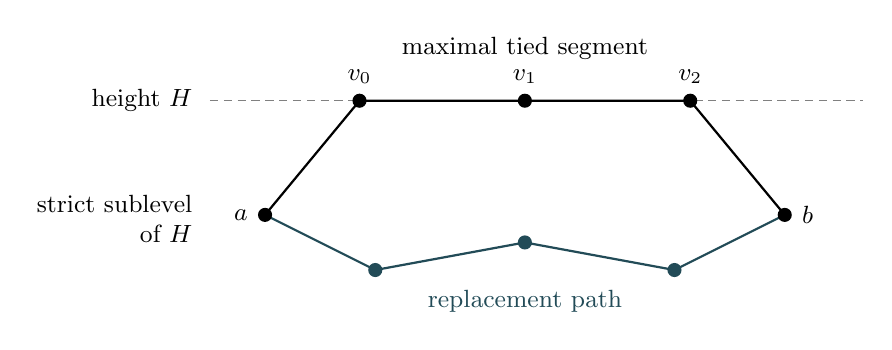
\begin{tikzpicture}[x=1cm,y=1cm,
  vertex/.style={circle,fill=black,inner sep=1.8pt},
  lower/.style={circle,fill=linkcolor,inner sep=1.8pt},
  every node/.style={font=\small}]
  \draw[densely dashed,gray] (-.7,1.35)--(7.6,1.35);
  \node[anchor=east] at (-.8,1.35) {height $H$};
  \node[anchor=east,align=right] at (-.8,-.15) {strict sublevel\\of $H$};
  \coordinate (a) at (0,-.1);
  \coordinate (b) at (6.6,-.1);
  \coordinate (v0) at (1.2,1.35);
  \coordinate (v1) at (3.3,1.35);
  \coordinate (v2) at (5.4,1.35);
  \draw[thick] (a)--(v0)--(v1)--(v2)--(b);
  \node[vertex,label=above:$v_0$] at (v0) {};
  \node[vertex,label=above:$v_1$] at (v1) {};
  \node[vertex,label=above:$v_2$] at (v2) {};
  \node at (3.3,2.02) {maximal tied segment};
  \coordinate (u0) at (1.4,-.8);
  \coordinate (u1) at (3.3,-.45);
  \coordinate (u2) at (5.2,-.8);
  \draw[thick,linkcolor] (a)--(u0)--(u1)--(u2)--(b);
  \foreach \p in {u0,u1,u2} {\node[lower] at (\p) {};}
  \node[vertex,label=left:$a$] at (a) {};
  \node[vertex,label=right:$b$] at (b) {};
  \node[text=linkcolor] at (3.3,-1.2) {replacement path};
\end{tikzpicture}

\caption{Lowering a maximal tied segment, as in
Proposition~\ref{ht:minima}.  Its two descending attachments $a,b$
belong to the same component of the strict height sublevel, so a
finite path there replaces the segment.  The drawing represents
comparability paths and a connectivity argument.}
\label{fig:tied-path}
\end{figure}

\begin{proof}
A minimum exists by Lemma~\ref{ht:well-order}.
Take a finite path between two minimum-height vertices in the
connected full graph.
If its greatest height is above the minimum, consider a maximal
contiguous segment at that height.
Consecutive vertices of the segment are comparable and tied.
The segment has descending attachments at its two ends.
Lemma~\ref{ht:ties} and Corollary~\ref{ht:descending} put these attachments
in one connected component of the strict sublevel.
Replace the segment by a finite path in that component.

Doing this for all segments at the current greatest height removes
that height entirely and introduces no vertex at or above it.
If the resulting path is still not a minimum path, repeat.
An infinite repetition would give a strictly descending sequence of
greatest heights, contrary to Lemma~\ref{ht:well-order}.
The process therefore ends with a path entirely among minima.
The constancy of \(K,T_+\) along its edges is Lemma~\ref{ht:ties}.
\end{proof}

\subsection{The stabilizer containment}

For later use define the simultaneous graded-homotopy stabilizer
\begin{equation}
 H(Y,x)=\{a\in A_Y:
 E_L(ax)\simeq E_L(x)\text{ for every simple label }L\}.
 \label{ht:stabilizer}
\end{equation}
This is a subgroup because the \(B_a\) are equivalences.
Choose a minimum \(v=(T,A_Tz)\), and abbreviate its invisible and visible
sets by \(K,T_+\).

\begin{proposition}[Containment from a minimum]
\label{ht:containment}
Put \(D=T_+\cup K\subseteq Y\).
The set \(T_+\) is spherical and nonadjacent to \(K\), and
\begin{equation}
 x^{-1}H(Y,x)x\subseteq z^{-1}A_Dz.
 \label{ht:containment-equation}
\end{equation}
Equivalently, with \(b=zx^{-1}\in A_Y\),
\(H(Y,x)\subseteq b^{-1}A_Db\).
\end{proposition}

\begin{proof}
The set \(T_+\) is contained in the spherical type \(T\).
Every visible closed color is positive at some recorded level, so
Equation~\eqref{ht:invisible} excludes adjacency to \(K\).

Along any minimum path starting at \(v\), the sets \(T_+,K,D\) are
constant by Proposition~\ref{ht:minima}, and every type is contained
in \(D\).
All cosets on that path lie in \(A_Dz\).
Indeed this holds initially because \(T\subseteq D\).
A downward inclusion preserves it; for an upward inclusion, the larger
coset has type contained in \(D\) and contains a point of \(A_Dz\), so
the whole larger coset also lies in \(A_Dz\).

Let \(a\in H(Y,x)\) and set \(r=x^{-1}ax\).
Right multiplication by \(r\) is an automorphism of the coset poset,
preserving types.  At a representative \(cx\), where \(c\in A_Y\),
\[
 E_L(cxr)=E_L(cax)\simeq B_cE_L(ax)
 \simeq B_cE_L(x)=E_L(cx).
\]
It therefore preserves all layer counts and heights.
The translated vertex \((T,A_Tzr)\) is a minimum, so
Proposition~\ref{ht:minima} joins it to \(v\) by a minimum path.
The coset containment along that path gives \(zr\in A_Dz\), hence
\(r\in z^{-1}A_Dz\), proving Equation~\eqref{ht:containment-equation}.
The equivalent formulation follows from \(z=bx\).
\end{proof}

\section{Bounded positive height in spherical colors}
\label{sec:spherical}

We now prove the containment needed for a stabilizer inside a spherical
standard parabolic.  If the tests on the operated colors are not all
acyclic, the stabilizer lies in a conjugate of a proper standard
parabolic.  In this case, the main step rules out an infinite sequence
of positive words, each containing every operated color, along which
total test height is bounded.

Suppose such a sequence existed.  Positive amplitude gives a fixed
lower bound on generator levels; bounded total test height and the
fixed exterior generators give a fixed upper bound.  Every member of
the family therefore has its generator levels in one interval
$[d_1,d_2]$.  Meanwhile the greatest ordinary cochain degree of tested
cohomology drops by at least one after each word.  We will convert the
resulting test vanishing on a long cochain interval below all exterior
generators into an empty cochain placement.  The finite path bound
below removes one layer after another, at a uniformly bounded cost in
placement.  At a sufficiently late stage, nonzero test cohomology still
lies below the empty placement and the fixed $f$-generator lies above
it.  One transported projective would split, contradicting its
indecomposability.

\subsection{A bound on coefficient paths}

The underlying path calculation is the essential-path construction
associated with Ocneanu and the Jones--Wenzl projections; see
\cite[Sections~3.1--3.2]{Coquereaux2002} and
\cite[Theorem~5.4.3 and Proposition~5.6.10]{Cooper2007}.
We give its projection argument explicitly so that the resulting
nilpotence bound can be applied on an interval of cochain placements,
where the coefficient maps may depend on the placement.

\begin{lemma}\label{sph:path-bound}
Let \(Y\subseteq S\) be spherical.  There is an integer \(N=N(Y)\geq1\)
with the following property.  Consider a minimal bounded complex
of projectives and an integer interval of cochain placements on
which all its generator vertices lie in \(\widetilde Y\).
In each pure layer, every composition of \(N\) successive arrow
coefficient maps vanishes, provided all \(N+1\) placements of the
composition lie in that interval.
\end{lemma}

\begin{proof}
By Lemma~\ref{cat:unfolding}, the graph on \(\widetilde Y\)
is a disjoint union of finite simply laced graphs whose Cartan
matrices are positive definite.  We first establish a path
identity on one connected component with an edge.
Write \(\mathsf B\) for its adjacency matrix.

There is a strictly positive vector \(\mu\) with
\[
 \mathsf B\mu=\delta\mu,\qquad 0<\delta<2.
\]
For completeness, maximize the Rayleigh quotient of
\(\mathsf B\) on the unit sphere.  Replacing a maximizing
vector by its coordinatewise absolute value does not decrease
the quotient.  The resulting nonnegative eigenvector is
strictly positive: the eigenvalue equation at a zero coordinate
would force its neighbors to be zero, and connectedness would
then force the entire vector to vanish.  An edge makes the
maximum eigenvalue positive, and positivity of
\(2I-\mathsf B\) makes it less than \(2\).

Choose opposite arrow bases on each edge so that the trace
of their product, in either order, is
\(\sqrt{\mu_i\mu_j}\).  The nondegenerate opposite-arrow pairing
and ordinary symmetry of the Frobenius trace allow this choice.
For coefficient maps of a pure layer, the length-two component
of the square of the differential is therefore the relation
\begin{equation}\label{sph:eq:path-relation}
 \sum_{j\sim i}\sqrt{\mu_j/\mu_i}\,(i\,j\,i)=0.
\end{equation}
Here a path denotes the corresponding composition of coefficient
maps, at successive cochain placements.  Indeed, before division
by \(\mu_i\), its coefficient in the token trace is
\(\sqrt{\mu_i\mu_j}\).  Minimality excludes length-zero
differential entries, so only two length-one entries contribute
to this part of \(d^2\).  The relation is valid on the prescribed
interval because every intervening generator there is in
\(\widetilde Y\).

We prove that all sufficiently long abstract paths lie in the
span of insertions of \eqref{sph:eq:path-relation}.
Let \(\mathcal V_n\) be the finite-dimensional Hilbert space
with orthonormal basis the paths \((a_0,\ldots,a_n)\) of length
\(n\).  For \(n\geq2\) and \(1\leq i\leq n-1\), define
\[
 c_i^{(n)}:\mathcal V_n\longrightarrow\mathcal V_{n-2}
\]
by zero unless \(a_{i-1}=a_{i+1}\).  On a backtrack
\((a,b,a)\) at these positions, delete its two edges and
multiply the shortened path by \(\sqrt{\mu_b/\mu_a}\).
The adjoint inserts exactly the weighted sum in
\eqref{sph:eq:path-relation}, with the surrounding path fixed.
All these maps preserve the two endpoints.

The contraction and insertion operators satisfy
\begin{align}
 c_i^{(n)}(c_i^{(n)})^*
     &=\delta\,\mathrm{id}_{\mathcal V_{n-2}},
       \label{sph:eq:loop}\\
 c_i^{(n)}(c_{i-1}^{(n)})^*
     &=c_{i-1}^{(n)}(c_i^{(n)})^*
       =\mathrm{id}_{\mathcal V_{n-2}}
       \quad(2\leq i\leq n-1).
       \label{sph:eq:adjacent}
\end{align}
In \eqref{sph:eq:loop}, the scalar at the insertion vertex
\(a\) is \(\sum_{b\sim a}\mu_b/\mu_a=\delta\).
For \eqref{sph:eq:adjacent}, the subsequent contraction
forces the inserted detour to use the adjacent edge already
present in the path.  Its two factors are reciprocal square
roots, so their product is \(1\).  In particular, both
identities in \eqref{sph:eq:adjacent} use the same ambient
length \(n\).

Let
\[
 \mathcal E_n=\bigcap_{i=1}^{n-1}\ker c_i^{(n)},
 \qquad
 \mathcal E_0=\mathcal V_0,\quad
 \mathcal E_1=\mathcal V_1,
\]
and let \(\Pi_n\) be the orthogonal projection onto
\(\mathcal E_n\).  Since these spaces decompose by endpoints,
\(\Pi_n\) preserves endpoints.  We may therefore extend
\(\Pi_k\) to longer path spaces by applying it to the first
\(k\) edges while keeping the tail fixed.

Write
\[
 \delta=2\cos\theta,\qquad 0<\theta<\pi/2,\qquad
 [u]=\frac{\sin(u\theta)}{\sin\theta},
 \qquad h=\min\{j\in\mathbb Z_{\geq1}:j\theta\geq\pi\}.
\]
Then \([n]>0\) for \(1\leq n<h\), and
\([n]=\delta[n-1]-[n-2]\).
For \(2\leq n<h\), denote by \(\mathsf Q_n\) the extension
of \(\Pi_{n-1}\) to the first \(n-1\) edges of a length-\(n\)
path.  We claim
\begin{equation}\label{sph:eq:scalar}
 c_{n-1}^{(n)}\mathsf Q_n(c_{n-1}^{(n)})^*
     =\frac{[n]}{[n-1]}\Pi_{n-2}
     \quad\hbox{on }\mathcal V_{n-2},
\end{equation}
and
\begin{equation}\label{sph:eq:projection}
 \Pi_n=\mathsf Q_n-
       \frac{[n-1]}{[n]}\,
       \mathsf Q_n(c_{n-1}^{(n)})^*
                    c_{n-1}^{(n)}\mathsf Q_n.
\end{equation}

At \(n=2\), \(\mathsf Q_2\) is the identity, and
\eqref{sph:eq:scalar} is \eqref{sph:eq:loop}, since
\([2]/[1]=\delta\).
To pass from \(n-1\) to \(n\), let \(\mathsf R_n\) be the
extension of \(\Pi_{n-2}\) to the first \(n-2\) edges.
Extending \eqref{sph:eq:projection} for \(n-1\) by one edge
gives
\[
 \mathsf Q_n=\mathsf R_n-
       \frac{[n-2]}{[n-1]}\,
       \mathsf R_n(c_{n-2}^{(n)})^*
                    c_{n-2}^{(n)}\mathsf R_n.
\]
Endpoint preservation gives the identities
\[
 c_{n-1}^{(n)}\mathsf R_n
       =\Pi_{n-2}c_{n-1}^{(n)},\qquad
 \mathsf R_n(c_{n-1}^{(n)})^*
       =(c_{n-1}^{(n)})^*\Pi_{n-2}.
\]
They concern \(\mathsf R_n\), whose prefix stops before the
last pair, not \(\mathsf Q_n\).
Substitution, followed by \eqref{sph:eq:loop} and the two
adjacent identities, yields
\begin{align*}
 c_{n-1}^{(n)}\mathsf Q_n(c_{n-1}^{(n)})^*
 &=\delta\Pi_{n-2}
   -\frac{[n-2]}{[n-1]}\,
     \Pi_{n-2}c_{n-1}^{(n)}(c_{n-2}^{(n)})^*
                c_{n-2}^{(n)}(c_{n-1}^{(n)})^*\Pi_{n-2}\\
 &=\left(\delta-\frac{[n-2]}{[n-1]}\right)\Pi_{n-2}\\
 &=\frac{[n]}{[n-1]}\Pi_{n-2}.
\end{align*}
This proves \eqref{sph:eq:scalar}.

To justify the projection formula, set
\(T_n=c_{n-1}^{(n)}\mathsf Q_n\).
The identity just proved reads
\[
 T_nT_n^*=\frac{[n]}{[n-1]}\Pi_{n-2}.
\]
In finite-dimensional Hilbert spaces, an operator and its
product with its adjoint have the same image: their
orthogonal complements are both the kernel of the adjoint.
Thus \(T_n\) maps onto \(\mathcal E_{n-2}\).
Restricted to \(\operatorname{im}\mathsf Q_n\), its kernel
is \(\mathcal E_n\), because the prefix projection has
already imposed all contractions except the last one.
To verify the projection explicitly, put
\(\lambda=[n]/[n-1]>0\).
The established range identity gives
\[
 (T_n^*T_n)^2=\lambda T_n^*T_n,\qquad
 \mathsf Q_nT_n^*T_n=T_n^*T_n
       =T_n^*T_n\mathsf Q_n.
\]
Consequently
\(\mathsf Q_n-\lambda^{-1}T_n^*T_n\) is self-adjoint
and idempotent.  It has image in
\(\operatorname{im}\mathsf Q_n\cap\ker T_n\) and is
the identity on that subspace.  This is the projection
\eqref{sph:eq:projection}, completing the induction.

It remains to prove that $\mathcal E_n$ vanishes for some $n$.
The endpoint-dimension recurrence below will give that finite path bound.
Let \(\mathsf d_n(i,j)\) be the dimension of
\(\mathcal E_n\) with endpoints \(i,j\).
Extending a path of length \(n-1\) by one edge makes the
endpoint-dimension matrix of
\(\operatorname{im}\mathsf Q_n\) equal to
\(\mathsf d_{n-1}\mathsf B\).
The restricted surjection
\(T_n:\operatorname{im}\mathsf Q_n\to\mathcal E_{n-2}\)
preserves endpoints and has kernel \(\mathcal E_n\).
Hence, for \(2\leq n<h\),
\[
 \mathsf d_n=\mathsf d_{n-1}\mathsf B-\mathsf d_{n-2},
 \qquad \mathsf d_0=I,\quad\mathsf d_1=\mathsf B.
\]
Multiplication by \(\mu\) and induction give
\(\mathsf d_n\mu=[n+1]\mu\).
In particular, the recursion is valid at \(n=h-1\).
No denominator \([h]\) has been used.
Since \(\pi\leq h\theta<\pi+\theta<3\pi/2\),
\[
 0\leq\mathsf d_{h-1}\mu=[h]\mu\leq0.
\]
The entries of \(\mathsf d_{h-1}\) are nonnegative and
\(\mu\) is strictly positive.  It follows that
\(\mathsf d_{h-1}=0\), and therefore
\(\mathcal E_{h-1}=0\).  The same equality also forces
\([h]=0\); no classification of the graph was needed.

In finite-dimensional inner product spaces,
\[
 \mathcal E_n^\perp
       =\sum_{i=1}^{n-1}\operatorname{im}(c_i^{(n)})^*.
\]
Thus every individual path of length \(h-1\) is a linear
combination of insertions of
\eqref{sph:eq:path-relation}.  Evaluate such an identity
on the coefficient maps, starting at any fixed cochain
placement in the prescribed interval.  Each inserted
relation is then a valid length-two part of \(d^2=0\)
at the corresponding placement.  The coefficient maps
may depend on the placement; no translation invariance
of them is required.  The entire composition vanishes.

For a connected component without an edge, use the bound
\(N=1\).  There are finitely many components; take the
maximum of their bounds.  A longer path factors through
an initial segment of the relevant vanishing length,
and no path crosses components.  The empty set \(Y\)
is vacuous and may also be assigned \(N=1\).
\end{proof}

\subsection{Two height bounds force a gap}

Fix now a nonempty spherical \(Y\subseteq S\) and \(x\in A\).
Write \(H^{p,u}(e_\alpha E)\) for the cohomology in ordinary
cochain degree \(p\) and internal degree \(u\).
For \(a\in A_Y\), define the total test height
\begin{equation}\label{sph:eq:height}
 h(a)=\max\{p+u:H^{p,u}(e_\alpha E_L(ax))\ne0
                  \text{ for some }\alpha\in\widetilde Y,L\},
\end{equation}
with value \(-\infty\) if all these tests vanish.
There are finitely many labels and vertices, and all the
complexes are bounded, so this maximum is finite whenever
it is nonempty.
For the moment suppose that \(h(1)\) is finite.
Lemma~\ref{lay:height-change} shows that it remains finite
and nondecreasing under positive words in \(A_Y^+\).

\begin{lemma}\label{sph:cochain-drop}
Suppose that all tests on \(\widetilde Y\) in a bounded
family have ordinary cochain cohomology in degrees at
most \(m\).  Positive operations in \(Y\) preserve this
bound.  After a positive word containing every color of
\(Y\), the bound improves to \(m-1\).
\end{lemma}

\begin{proof}
For an acted vertex, Lemma~\ref{lay:positive} gives the
test shift \(\langle2\rangle[1]\), which lowers the
ordinary cochain bound by one.
At an unacted vertex \(\beta\), applying the vertex test
to the evaluation cone gives a triangle
\[
 \bigoplus_{\alpha\in\widetilde{\{i\}}}
      e_\beta P_\alpha\otimes_{\kk}e_\alpha E
       \longrightarrow e_\beta E
       \longrightarrow e_\beta F_iE .
\]
When \(\beta\) is adjacent to color \(i\), the first term
is a sum of acted tests shifted only in internal degree,
because each \(e_\beta P_\alpha\) is an arrow space.
It consequently has ordinary cochain cohomology at
most \(m\).  The long exact sequence gives zero above
\(m\) for the new test and a surjection
\[
 H^m_{\mathrm{coch}}(e_\beta E)
       \longrightarrow H^m_{\mathrm{coch}}(e_\beta F_iE),
\]
where each group retains its internal grading.
For a nonneighbor the first term vanishes and the test
is unchanged.

Thus once cohomology at degree \(m\) has vanished at a
vertex, later operations at other colors cannot restore
it: the later groups in that degree are quotients of
zero.  Another operation at its own color still gives
zero in degree \(m\), using the bound above \(m\).
After every color has been operated, degree \(m\) has
vanished everywhere.  The vertices of a single color
are pairwise nonadjacent, so the simultaneous color
operation satisfies the same conclusions.
\end{proof}

\begin{lemma}\label{sph:empty-placement}
Let a minimal bounded projective complex have generator
levels in \([d_1,d_2]\).  Suppose that on an integer
cochain interval \([l,r]\) all its generators lie in
\(\widetilde Y\), and all vertex tests on
\(\widetilde Y\) have zero cohomology in each ordinary
cochain degree in this interval, in every internal
degree.  With \(N=N(Y)\) from Lemma~\ref{sph:path-bound},
there are no generators at any placement
\[
 l+N(d_2-d_1+1)\leq p\leq r.
\]
\end{lemma}

\begin{proof}
Fix a vertex and a generator coefficient in layer \(d_2\)
at placement \(p\), with \(l<p\leq r\).
Multiplying its projective generator by its token gives
a cycle in the corresponding vertex test.  Every
differential entry is of positive path length and every
product of a token with such an entry is zero.
The tested cohomology vanishes at \(p\), so this token
coefficient is a boundary from placement \(p-1\).

Project such a boundary onto its token coefficient
space.  A length-one differential entry can contribute
only through an opposite arrow in the test, giving an
incoming arrow-coefficient image from the same layer.
A length-two entry can contribute only through a unit
path, and its source generator would lie in layer
\(d_2+1\).  This latter layer is absent.
These exhaust the possibilities, since minimality
excludes length-zero entries.  The perfect
opposite-arrow pairing therefore shows that the full
coefficient space at placement \(p\) is spanned by
incoming arrow-coefficient images at \(p-1\).

For \(p\geq l+N\), iterate this spanning assertion \(N\)
times.  Every path involved has its placements in
\([l,r]\), so Lemma~\ref{sph:path-bound} makes its
coefficient composition zero.  Layer \(d_2\) is
therefore empty for \(l+N\leq p\leq r\).

Proceed downward through the layers.  Suppose that
the higher layers have already been removed on
\([l+jN,r]\).  For layer \(d_2-j\) and
\(p>l+jN\), a possible token source from the next
higher layer at \(p-1\) is absent on that interval.
The same argument expresses the coefficient space
by incoming arrows, and then by \(N\)-step paths.
It removes this layer on \([l+(j+1)N,r]\).
The successive conclusions are
\[
 \begin{array}{c|c}
 \text{layer}&\text{interval proved empty}\\ \hline
 d_2 &[l+N,r]\\
 d_2-1 &[l+2N,r]\\
 \vdots&\vdots\\
 d_1 &[l+N(d_2-d_1+1),r].
 \end{array}
\]
On the last interval every possible generator layer
has been removed, proving the assertion.
\end{proof}

\begin{proposition}\label{sph:no-chain}
Assume \(h(1)>-\infty\).
There is no sequence
\[
 a_0=1,\qquad a_{k+1}=w_k a_k,\qquad
 w_k\in A_Y^+,\quad\operatorname{supp}(w_k)=Y,
\]
for which the integers \(h(a_k)\) have a common upper
bound.
\end{proposition}

\begin{proof}
Suppose that \(h(a_k)\leq h_*\) for all \(k\).
Choose a common lower bound \(d_1\) on the generator
levels of the initial family \(E_L(x)\).
Positive amplitude, Lemma~\ref{lay:positive} and the
bounded-layer formalism of Lemma~\ref{lay:structure},
preserves this bound at every stage.

All generator placements outside \(Y\) are fixed by
the family properties in Proposition~\ref{cat:family}.
Let \(d_{\mathrm{ext}}\) be their largest occupied
level.  The exterior includes the unchanged f
generator at placement \((0,0)\), so this is defined.
If a current global highest layer has degree
\(d>d_{\mathrm{ext}}\), it is supported entirely in
\(\widetilde Y\).  A nonzero such layer has a nonzero
top: incoming coefficient maps increase cochain
placement in a finite array and cannot generate a
nonzero array indefinitely.  Lemma~\ref{lay:extremal}
then gives a nonzero test in total degree \(d+2\).
It follows that every current generator has level
in the fixed interval
\[
 [d_1,d_2],\qquad
 d_2=\max(d_{\mathrm{ext}},h_*-2).
\]

By Lemma~\ref{sph:cochain-drop}, the common upper bound
on ordinary cochain test cohomology drops by at least
one at every step \(a_k\to a_{k+1}\).
It therefore tends to \(-\infty\).
Let \(p_{\mathrm{ext}}\) be the least exterior
generator cochain placement, over the initial finite
family.  It is fixed, and \(p_{\mathrm{ext}}\leq0\)
because of the f generator.
Set
\[
 N=N(Y),\quad
 K_0=N(d_2-d_1+1),\quad
 r=p_{\mathrm{ext}}-1,\quad l=r-K_0.
\]
At a sufficiently late stage all tested cohomology
on \(\widetilde Y\) lies in cochain degrees strictly
below \(l\).  Every generator in \([l,r]\) lies in
\(\widetilde Y\), since \(r<p_{\mathrm{ext}}\).
Lemma~\ref{sph:empty-placement} consequently shows
that every member of the family has no term at
cochain placement \(r=l+K_0\).

Some member nevertheless has nonzero test cohomology,
by positive height monotonicity from \(h(1)>-\infty\).
For that member there is a term in a cochain degree
below \(l\), while its unchanged f generator is in
degree \(0>r\).
The absent term in degree \(r\) splits its minimal
complex into two nonempty bounded minimal complexes,
one on either side of that degree.
Neither summand is contractible.  Indeed a contracting
homotopy would express its identity as \(dh+hd\);
every component of the latter lies in the additive
radical because all entries of \(d\) do.  Reduction
modulo the radical would give a nonzero identity
equal to zero.
This contradicts the indecomposability of
\(E_L(a_kx)\) from Proposition~\ref{cat:family}.
\end{proof}

\subsection{Positive extensions and a proper support}

\begin{lemma}\label{sph:common-extension}
For \(a,b\in A_Y\), there are \(p,q\in A_Y^+\) and
\(u\in A_Y\) such that
\[
 u=pa=qb,\qquad h(u)\leq\max(h(a),h(b)).
\]
The same upper bound holds for a common positive
left extension of any finite family.
\end{lemma}

\begin{proof}
The finite-type fraction property in
Theorem~\ref{cat:classical} first gives \(u=pa=qb\)
with \(p,q\) positive.  Whenever \(p\) and \(q\)
have a common left atom, write
\(p=\sigma_i p'\), \(q=\sigma_i q'\) and cancel it.
This replaces the common extension by
\(p'a=q'b\).
The sum of positive lengths decreases by two, so
the process terminates with no common left atom.

Suppose the resulting extension satisfies
\(h(u)>\max(h(a),h(b))\).
Choose one label \(L\) and one unfolded vertex
\(\alpha\in\widetilde Y\) attaining \(h(u)\) for
\(E_L(ux)\).
For this same family member, its starting test
height on each side is smaller than \(h(u)\).
If one starting set of tests vanished, persistence
of vanishing under positive words would contradict
the final nonzero test.  Otherwise
Lemma~\ref{lay:top-divisor} applies to each side.
It makes \(\alpha\) a left divisor of both unfolded
positive words.

Lemma~\ref{two:greedy} reflects this divisibility
to a common original color.  In its right-divisor
form this lemma is transferred to left divisors
by word reversal: every Artin braid relation is
preserved by reversal, and a color unfolds to a
product of commuting letters whose reversal
represents the same element.
Thus the original positive elements \(p,q\) have
a common left atom, a contradiction.
This proves the stated inequality.
Repeated pairwise application constructs a common
extension of any finite family, with height no
larger than the maximum of its starting heights.
\end{proof}

Positive support is well defined on \(A_Y^+\):
the positive monoid embeds, and every positive
Artin relation preserves the set of colors
occurring in a word.  In particular, the support
of a positive divisor is contained in the support
of the element it divides.

\begin{lemma}\label{sph:proper-support}
Assume \(h(1)>-\infty\), and put \(h_0=h(1)\).
There exist \(p\in A_Y^+\) with \(h(p)\leq h_0\)
and one proper subset \(J\subsetneq Y\) such that
\[
 b\in A_Y^+,\quad h(bp)\leq h_0
       \quad\Longrightarrow\quad
       \operatorname{supp}(b)\subseteq J.
\]
\end{lemma}

\begin{proof}
If no such \(p\) existed, then for every positive
\(p\) with \(h(p)\leq h_0\) the union of supports
of all its permitted continuations would equal
\(Y\).
For each color \(i\in Y\), choose a continuation
\(b_i\) whose support contains \(i\) and for which
\(h(b_i p)\leq h_0\).
Lemma~\ref{sph:common-extension} gives a common
positive left extension of these endpoints:
\[
 u=c_i b_i p\quad(i\in Y),\qquad
 c_i\in A_Y^+,\qquad h(u)\leq h_0.
\]
Cancelling \(p\) shows that \(w=up^{-1}=c_i b_i\)
is a positive element independent of \(i\).
Every \(b_i\) is a right divisor of \(w\), so
\(\operatorname{supp}(w)=Y\).
This constructs a new positive endpoint \(wp\)
with height at most \(h_0\).
At every intermediate letter of this operation
the height also stays at most \(h_0\), by positive
monotonicity.

Starting from \(p=1\) and repeating gives an
infinite sequence forbidden by
Proposition~\ref{sph:no-chain}.
Therefore some \(p\) has a proper union of the
supports of all its permitted continuations.
Take \(J\) to be precisely that union.
This establishes one common proper subset,
not merely a separately missing color for
each continuation.
\end{proof}

\begin{proposition}\label{sph:containment}
Let \(Y\subseteq S\) be spherical and \(x\in A\).
For the family stabilizer
\[
 H(Y,x)=\{s\in A_Y:E_L(sx)\simeq E_L(x)
                         \text{ for every }L\},
\]
one of the following holds:
\begin{enumerate}
 \item all tests on \(\widetilde Y\) at \(x\)
       are acyclic and \(H(Y,x)=A_Y\);
 \item there exist \(p\in A_Y^+\) and
       \(J\subsetneq Y\) such that
       \begin{equation}\label{sph:eq:containment}
        H(Y,x)\subseteq p^{-1}A_Jp .
       \end{equation}
\end{enumerate}
\end{proposition}

\begin{proof}
Suppose first that some test is nonzero.
Use \(p,J\) from Lemma~\ref{sph:proper-support}.
For \(s\in H(Y,x)\), the equivalences of family
members are preserved by every prefix of the
action.  In particular
\[
 h(ps)=h(p),\qquad h(bps)=h(bp)
                   \quad(b\in A_Y^+).
\]
Apply Lemma~\ref{sph:common-extension} to
\(p,ps\), obtaining
\[
 ap=bps,\qquad a,b\in A_Y^+,\qquad
 h(ap)=h(bps)\leq h(p)\leq h_0.
\]
Thus \(a\) is a permitted continuation of \(p\).
The equality \(h(bp)=h(bps)\) shows that \(b\)
is also permitted.  Both have support in \(J\),
so
\[
 s=p^{-1}b^{-1}ap\in p^{-1}A_Jp.
\]
This proves \eqref{sph:eq:containment}.

If all the tests are acyclic, the evaluation
term for each positive color twist is a bounded
acyclic complex of graded vector spaces tensored
with projectives.  It is contractible, since a
bounded acyclic vector-space complex splits
degreewise, in each internal degree.
The evaluation cone is consequently equivalent
to the original family member.
Every positive generator fixes the family, and
its inverse fixes it as well by applying the
inverse equivalence.
The generators therefore give
\(H(Y,x)=A_Y\).
This argument includes \(Y=\varnothing\), when
there are no tests and the group is trivial.
\end{proof}

\section{Stabilizers and parabolic intersections}
\label{sec:stabilizers}

We now combine the two containment arguments. Throughout this section,
$X\subseteq S$ and its relative family are fixed. The element $x\in A$
is arbitrary; in particular, it need not belong to the subgroup that
is currently acting.

\begin{lemma}[Conjugating a stabilizer]
\label{stab:conjugation}
Let $D\subseteq Y\subseteq S$ and $b\in A_Y$. If
$H(Y,x)\subseteq b^{-1}A_Db$, then
\[
 bH(Y,x)b^{-1}=H(D,bx).
\]
\end{lemma}
\begin{proof}
For $c\in A_D$, invertibility of $B_b$ gives
\[
 E_L(cbx)\simeq E_L(bx)\quad\text{for all }L
 \quad\Longleftrightarrow\quad
 E_L(b^{-1}cbx)\simeq E_L(x)\quad\text{for all }L.
\]
Since $b^{-1}cb\in A_Y$, the right side says that
$b^{-1}cb\in H(Y,x)$. Thus
$H(D,bx)=A_D\cap bH(Y,x)b^{-1}$. The assumed containment removes the
intersection.
\end{proof}

\begin{theorem}[Relative stabilizers are parabolic]
\label{stab:parabolic}
For every $Y\subseteq S$ and $x\in A$, there exist $R\subseteq Y$ and
$c\in A_Y$ such that
\[
 H(Y,x)=c^{-1}A_Rc.
\]
\end{theorem}
\begin{proof}
We induct on $|Y|$, allowing every $x\in A$ at every rank. The assertion
is immediate for $Y=\varnothing$. By Lemma~\ref{stab:conjugation}, it
suffices to place $H(Y,x)$ inside $b^{-1}A_Db$ for some $b\in A_Y$ and
proper $D\subsetneq Y$: the conjugated stabilizer is then $H(D,bx)$,
to which induction applies.

Suppose first that $Y$ is spherical. If all its tests on the family at
$x$ are acyclic, every generator in $Y$ fixes every member, so
$H(Y,x)=A_Y$. Otherwise Proposition~\ref{sph:containment} gives the
required proper-type containment.

Now suppose that $Y$ is nonspherical. Choose a minimum vertex
$P=(T,A_Tz)$ of the relative harmonic filtration of $A_Yx$. Let $K$ be
its invisible set and put $T_+=T\setminus K$, as in
Section~\ref{sec:heights}. Proposition~\ref{ht:containment} gives
\[
 x^{-1}H(Y,x)x\subseteq z^{-1}A_Dz,
 \qquad D=T_+\cup K\subseteq Y.
\]
Since $z\in A_Yx$, the element $b=zx^{-1}$ belongs to $A_Y$, and this
is exactly $H(Y,x)\subseteq b^{-1}A_Db$. If $D\ne Y$, the induction
step is complete.

It remains to treat $D=Y$. The sets $T_+$ and $K$ are disjoint and
nonadjacent, and $T_+$ is spherical because it is a subset of $T$.
We claim that the entire $K$-factor fixes the family at $x$.

Let $j\notin Y$ be an exterior neighbor of $K$. At every recorded level,
the definition of $K$ makes its harmonic coordinate zero. Outside $Y$
these coordinates are actual generator counts, fixed throughout $A_Yx$.
The cutoff was chosen at or below \emph{every} occupied exterior level,
so there are no generators of color $j$ at any level, for any member
of the family at any $w\in A_Yx$. There is also no
edge from $K$ to $T_+=Y\setminus K$. If a member $E_L(w)$ had a generator
in $K$, its connected color support, which contains $f\notin Y$, would
have to cross an exterior neighbor of $K$. We have just excluded every
such generator. This applies in particular at $w=x$: the family there
has no generators in $K$ or any of its neighbors, even at levels below
the cutoff.

Every test at a color of $K$ is therefore zero termwise. The evaluation
cone shows that its positive generator fixes each member, and its inverse
does so as well. The Artin presentation and standard embedding give
\[
 A_Y=A_K\times A_{T_+},
 \qquad H(Y,x)=A_K\times H(T_+,x).
\]
Since $Y$ is nonspherical, the spherical subset $T_+$ is proper.
Induction supplies $R\subseteq T_+$ and $c\in A_{T_+}$ with
$H(T_+,x)=c^{-1}A_Rc$. Commutation with $A_K$ now gives
\[
 H(Y,x)=c^{-1}(A_K\times A_R)c=c^{-1}A_{K\cup R}c.
\]
This also covers $T_+=\varnothing$.
\end{proof}

\begin{proposition}[The initial stabilizer]
\label{stab:initial}
The relative family associated with $X$ satisfies $H(S,1)=A_X$.
\end{proposition}
\begin{proof}
Every color of $X$ is nonadjacent to $f$. Its evaluation on every
$P_{f,L}$ is zero, so its twist fixes that projective. This proves
$A_X\subseteq H(S,1)$.

Consider the filtration for $Y=S$ and $x=1$. The empty-type vertex
$P_0=(\varnothing,\{1\})$ has only one nonzero layer vector, namely
the unit vector at $f$ in level zero. This vertex has minimum height.
Indeed a competitor with any nonzero higher block is later. At level
zero, every competitor retains the exterior coordinate $p_f^0=1$, and
all coordinates are nonnegative. Its coordinate sum is therefore at
least one. Equality forces its entire vector to be the unit vector at
$f$, and then every closed-type sign coordinate is zero, since the
type lies in $S$. Every lower block of $P_0$ is zero and is least.

At this minimum $T_+=\varnothing$. A color of $S$ is invisible precisely
when it is nonadjacent to $f$, so $K=X$. Applying
Proposition~\ref{ht:containment} with $z=x=1$ gives
$H(S,1)\subseteq A_X$.
\end{proof}

\begin{proof}[Proof of Theorem~\ref{thm:main}]
Simultaneous conjugation reduces the assertion to the intersection
$A_X\cap x^{-1}A_Yx$, with $x\in A$. For $a\in A_Y$, invertibility
of $B_x$ and Proposition~\ref{stab:initial} give
\begin{align*}
 x^{-1}ax\in A_X
 &\ \Longleftrightarrow\ 
 E_L(x^{-1}ax)\simeq E_L(1)\quad\text{for every }L\\
 &\ \Longleftrightarrow\ 
 E_L(ax)\simeq E_L(x)\quad\text{for every }L\\
 &\ \Longleftrightarrow\ a\in H(Y,x).
\end{align*}
Consequently
\[
 A_X\cap x^{-1}A_Yx=x^{-1}H(Y,x)x.
\]
By Theorem~\ref{stab:parabolic}, write $H(Y,x)=c^{-1}A_Zc$ with
$Z\subseteq Y$ and $c\in A_Y$. The displayed intersection is then
$(cx)^{-1}A_Z(cx)$, hence is parabolic. Conjugating back proves the
assertion for the originally specified $g$ and $h$.
\end{proof}


\subsection{Parabolic closure and dynamics}
\label{sec:consequences}

The inside-parabolic description obtained above makes the rank decrease
in an intersection explicit. We use it to prove the introductory
consequences, then record the fixed-point and continuity implications.

\begin{proof}[Proof of Corollary~\ref{cor:arbitrary-intersections}]
If $Q=gA_Yg^{-1}$ and $P=hA_Xh^{-1}$, put $x=g^{-1}h$. The proof of
Theorem~\ref{thm:main} and Theorem~\ref{stab:parabolic} give
\[
 Q\cap P=g c^{-1}A_Rc g^{-1}
 \quad\text{for some }R\subseteq Y\text{ and }c\in A_Y.
\]
If this intersection is strictly smaller than $Q$, then $R\ne Y$, since
conjugation by $c\in A_Y$ preserves $A_Y$. Thus a strict intersection step
decreases the size of the displayed defining set.

Start with $Q=A=A_S$ and no selected members of $\mathcal F$. Whenever $Q$
is not contained in some $P\in\mathcal F$, replace $Q$ by $Q\cap P$ and
select that member. The preceding strict decrease permits at most $|S|$
steps. The resulting $Q$ is contained in every member of $\mathcal F$ and
is the intersection of the selected subfamily, proving the displayed
equality and parabolicity. Finally, the family of parabolics containing
$E$ is nonempty because it contains $A$; its intersection is the unique
smallest such subgroup.
\end{proof}

\begin{proof}[Proof of Corollary~\ref{cor:nonclique-dynamics}]
In the presentation graph in which every finite label is an edge, the
infinite-label pair gives the visual splitting over
$A_{S\setminus\{s,t\}}$ of
\cite[Definition~2.4]{CharneyMartinMorrisWright2026}.
Theorem~\ref{thm:main} makes intersections of two conjugates of this edge
group parabolic in $A$. Hence
\cite[Theorem~3.2]{CharneyMartinMorrisWright2026} gives acylindrical
hyperbolicity and weak malnormality of the edge group, and
\cite[Proposition~4.2]{CharneyMartinMorrisWright2026} gives weak malnormality
of every proper parabolic.

The finite intersection supplied by weak malnormality is parabolic by
Theorem~\ref{thm:main}. A nontrivial parabolic contains a conjugate of
some $\sigma_s$, which has infinite order: the exponent-sum homomorphism
$A\to\mathbb Z$ sends every standard generator to $1$. Thus a finite
parabolic is trivial, giving the stated witness.
\end{proof}

\subsection{Fixed-point subgroups and locally compact groups}
\label{sec:fixed-point-consequences}

A parabolic subgroup is \emph{complete} if it is conjugate to $A_T$
for a set $T$ with no infinite label; it need not be spherical.
A group has property $\mathrm{FA}'$ if, in every simplicial action on a
tree without inversions, each element fixes a vertex. A locally compact
Hausdorff group $L$ is \emph{almost connected} if $L/L^\circ$ is compact.
A discrete group is \emph{lcH-slender} if every abstract homomorphism
into it from a locally compact Hausdorff group is continuous.

\begin{corollary}[Reduction to complete parabolics]
\label{cor:complete-parabolics}
Let $A=A_M$ with $S$ finite.
\begin{enumerate}
\item Every subgroup of $A$ with property $\mathrm{FA}'$ lies in a
complete parabolic subgroup.
\item Every abstract homomorphism $L\to A$ from an almost-connected
locally compact Hausdorff group has image in a complete parabolic.
\item If every complete standard parabolic of $A$ is lcH-slender,
then $A$ is lcH-slender.
\end{enumerate}
\end{corollary}
\begin{proof}
Theorem~\ref{thm:main} places $A$ in the class of groups whose parabolics
are closed under pairwise intersections. Apply
\cite[Proposition~1.3 and Theorem~1.7]{MoellerParisVarghese2024}.
\end{proof}


\subsection{Faithfulness and effective membership}
\label{sec:algorithms}

The unit-label projective already detects membership in $A_X$. Indeed,
label compatibility in Proposition~\ref{cat:family} and the initial
stabilizer calculation give
\begin{equation}
 B_wP_{f,\mathbf1}\simeq P_{f,\mathbf1}
 \quad\Longleftrightarrow\quad w\in A_X.
 \label{stab:single-detector}
\end{equation}
For the forward implication, tensoring labels by each simple $L$ gives
$B_wP_{f,L}\simeq P_{f,L}$, so Proposition~\ref{stab:initial} applies.
The reverse implication follows from the same proposition.
In particular, for $X=\varnothing$ the constructed action is faithful:
an element acting by the identity functor fixes $P_{f,\mathbf1}$ and
is therefore the identity of $A$. This is the action for our framed,
per-edge-labelled algebra; the faithfulness question for the original
unframed construction of \cite[Conjecture~7.10]{HengLicata2024} concerns
a different category.

To make \eqref{stab:single-detector} an algorithm, we must compute in the
chosen algebra exactly. The related twist-group algorithm of
\cite[Proposition~7.11]{HengLicata2024} also uses Gaussian elimination.
We give the coefficient-field construction here, so finite-dimensionality
over $\mathbb C$ is not being used as an effectiveness assumption.

\begin{proof}[Proof of Corollary~\ref{cor:membership}]
Fix the supplied $M$ and $X$, and use their relative construction.
Let $N$ be the least common multiple of the integers $2m$ for finite
edge labels $m\ge4$, and take $K=\mathbb Q(\exp(2\pi i/N))$; take
$K=\mathbb Q$ if there is no such label. Then $K$ contains every
parameter $q_m=\exp(\pi i/m)$. This field and its exact arithmetic are
computable from the finite matrix $M$.

We realize each Temperley--Lieb--Jones factor in its planar model.
Loop-free pairing diagrams give finite bases for each required underlying
planar morphism space; stacking diagrams evaluates every closed loop as $q_m+q_m^{-1}$.
The Jones--Wenzl recursion computes the simple idempotents
$p_0,\ldots,p_{m-2}$ over $K$, with nonzero denominators in this range
\cite[Definition~2.1.1, Remark~2.1.3, and Theorem~2.3.2]{Chen2014}.
Negligible maps are kernels of finite trace-pairing matrices, so their
quotient spaces and basis reductions are obtained by exact linear
algebra. For idempotents $p,q$, their corner morphism space is the image
of $f\mapsto qfp$ in that quotient
\cite[Definition~2.4.1, Lemma~2.4.3, and Definition~5.2.1]{Chen2014}.
Composition, tensoring and pivotal evaluation are consequently
computable in these finite diagram spaces. These finite kernels,
quotients and corner images commute with scalar extension to
$\mathbb C$, recovering the model used in Section~\ref{sec:category}.

The known simple list also makes decomposition effective. For any
object $U$ needed in a product, compute bases of
$\Hom(p_a,U)$ and $\Hom(U,p_a)$. Their composition pairing takes values
in $\End(p_a)=K$ and is nondegenerate; invert its matrix to obtain dual
inclusions and projections. The sum of the resulting simple-block
projections is $\mathrm{id}_U$, by the complete semisimple decomposition
of \cite[Theorems~5.4.4--5.4.5]{Chen2014}. These identities hold over
$K$: they hold after extension to $\mathbb C$, and scalar extension is
faithful. Thus no search for an unspecified categorical decomposition
is required. Finite products of the factors and direct sums are handled
by tensor products and matrices of these maps.

It follows that every space
$\Hom(L,D^a_{ij}\otimes H)$ and every multiplication map defining $Z$
has computable structure constants over $K$. Let $Z_K$ denote this
finite algebra. Its trace weights belong to $K$, and matrix inversion
computes trace-dual bases, hence the coevaluation maps as well as the
evaluation maps. All terms and differentials of $B_i,D_i$ are now
explicit over $K$. Unnormalized planar bases suffice; the square-root
normalization used only in the proof of Lemma~\ref{sph:path-bound}
is not needed for this construction.

Given the input words $u,v$, form the word $w=u^{-1}vu$ and compute the
bounded projective complex $B_wP_{f,\mathbf1}$ by finite tensor products.
Cancel invertible scalar differential entries between equal shifted
projectives until none remain, as in Section~\ref{sec:layers}. Each
cancellation uses exact arithmetic in $K$ and removes two summands,
so the process terminates.

The positive-path-length ideal of $Z_K$ is nilpotent and its quotient is
a product of copies of $K$. It is therefore the radical, and it remains
the radical after extension to $\mathbb C$. The computed minimal complex
stays minimal under that extension. By uniqueness of minimal models,
it is equivalent over $\mathbb C$ to $P_{f,\mathbf1}$ precisely when its
only generator is that projective in placements $(0,0)$. This is a finite
check of its summands; when it succeeds there is no differential left.
Equation~\eqref{stab:single-detector} identifies success with $w\in A_X$,
equivalently $v\in uA_Xu^{-1}$. Taking $X=\varnothing$ decides whether a
word is the identity, and applying this test to the quotient of two words
decides their equality.
\end{proof}


\begingroup
\small
\bibliographystyle{plain}
\bibliography{references}
\endgroup
\end{document}
